\documentclass[12pt,a4paper,oneside]{report}

\usepackage{mathptmx}
\usepackage[T1]{fontenc}
\usepackage[utf8]{inputenc}
\usepackage[main=english,ngerman]{babel}
\usepackage{csquotes}

\usepackage{microtype}

\usepackage[a4paper,left=2.5cm,right=2.5cm,top=2.5cm,bottom=3cm]{geometry}
\usepackage{setspace}
\setstretch{1.25}

\usepackage{parskip}

\usepackage{titlesec}
\newif\ifrunningbodychapters
\makeatletter
\patchcmd{\chapter}{\if@openright\cleardoublepage\else\clearpage\fi}%
  {\ifrunningbodychapters\par\else\if@openright\cleardoublepage\else\clearpage\fi\fi}{}{}
\makeatother
\titleformat{\chapter}[hang]{\normalfont\huge\bfseries}{\thechapter}{1em}{}
\titlespacing*{\chapter}{0pt}{1.2ex plus .3ex minus .2ex}{0.6ex plus .2ex}
\titlespacing*{\section}{0pt}{1.2ex plus .3ex minus .2ex}{0.6ex plus .2ex}
\titlespacing*{\subsection}{0pt}{1.2ex plus .3ex minus .2ex}{0.6ex plus .2ex}
\titlespacing*{\subsubsection}{0pt}{1.2ex plus .3ex minus .2ex}{0.6ex plus .2ex}

\titleformat{\paragraph}[runin]{\normalfont\normalsize\bfseries}{}{0pt}{}
\titlespacing*{\paragraph}{0pt}{2.2ex plus .6ex minus .2ex}{1em}

\setcounter{secnumdepth}{3}
\setcounter{tocdepth}{2}

\setlength{\parskip}{0.3\baselineskip plus 1pt minus 1pt}

\setlength{\floatsep}{8pt plus 2pt minus 2pt}
\setlength{\textfloatsep}{10pt plus 2pt minus 3pt}
\setlength{\intextsep}{8pt plus 2pt minus 2pt}
\setlength{\abovecaptionskip}{5pt}
\setlength{\belowcaptionskip}{0pt}

\usepackage{enumitem}
\setlist{itemsep=1pt, parsep=1pt, topsep=3pt, partopsep=0pt}

\renewcommand{\topfraction}{0.9}
\renewcommand{\bottomfraction}{0.7}
\renewcommand{\textfraction}{0.08}
\renewcommand{\floatpagefraction}{0.75}
\widowpenalty=8000
\clubpenalty=8000

\usepackage{url}
\urlstyle{tt}

\usepackage{emptypage}

\usepackage{array}
\usepackage{booktabs}
\usepackage{tabularx}
\usepackage{longtable}
\usepackage{multirow}
\usepackage{graphicx}
\usepackage{float}
\usepackage{rotating}
\usepackage{caption}
\captionsetup{font=small,labelfont=bf}
\newcommand{\tabnote}[1]{\par\vspace{2pt}\footnotesize\textit{Note.} #1}

\usepackage{amsmath}
\usepackage{amssymb}

\usepackage{listings}
\usepackage{xcolor}
\definecolor{codegray}{gray}{0.95}
\definecolor{codekw}{RGB}{0,80,160}
\definecolor{codecomment}{RGB}{110,110,110}
\lstdefinelanguage{SPARQL}{
  morekeywords={SELECT,DISTINCT,WHERE,FILTER,OPTIONAL,UNION,GROUP,BY,ORDER,
                LIMIT,SERVICE,VALUES,MINUS,EXISTS,COUNT,ASK,PREFIX,AS,DESC,
                BIND,HAVING},
  sensitive=false,
  morecomment=[l]{\#},
  morestring=[b]",
}
\lstset{
  basicstyle=\ttfamily\footnotesize,
  backgroundcolor=\color{codegray},
  keywordstyle=\color{codekw}\bfseries,
  commentstyle=\color{codecomment}\itshape,
  breaklines=true,
  frame=single,
  framesep=4pt,
  rulecolor=\color{gray!40},
  captionpos=b,
  columns=fullflexible,
  extendedchars=true,
  inputencoding=utf8,
  literate={—}{{---}}1 {–}{{--}}1 {§}{{\S}}1
           {‘}{{`}}1 {’}{{'}}1 {“}{{``}}1 {”}{{''}}1
           {…}{{\ldots}}1 {é}{{\'e}}1 {ü}{{\"u}}1
           {ö}{{\"o}}1 {ä}{{\"a}}1 {ß}{{\ss}}1,
}

\usepackage[backend=biber,style=numeric,natbib=true]{biblatex}
\addbibresource{references.bib}
\setcounter{biburlnumpenalty}{7000}
\setcounter{biburlucpenalty}{7000}
\setcounter{biburllcpenalty}{7000}

\AtEveryBibitem{\clearfield{note}}
\renewcommand*{\bibfont}{\small}
\setlength{\bibitemsep}{0.4\baselineskip}

\usepackage[colorlinks=true,linkcolor=black,citecolor=black,filecolor=black,urlcolor=blue]{hyperref}
\usepackage[capitalise,noabbrev]{cleveref}

\makeatletter
\let\thesis@addcontentsline\addcontentsline
\renewcommand{\addcontentsline}[3]{%
  \ifstrequal{#2}{paragraph}{}{\thesis@addcontentsline{#1}{#2}{#3}}%
}
\makeatother

\newcommand{\qid}[1]{\texttt{#1}}
\newcommand{\prop}[1]{\texttt{#1}}
\newcommand{\method}{stage-wise diagnostic evaluation}
\newcommand{\Method}{Stage-wise diagnostic evaluation}

\begin{document}

\newif\ifdeclarationupfront
\declarationupfronttrue

\pagenumbering{roman}
\begin{titlepage}
\centering
\setstretch{1}
\setlength{\parskip}{0pt}
\vspace*{0.6cm}


\includegraphics[width=8cm]{figures/leuphana_logo.jpg}

\vspace{1.8cm}

{\LARGE\bfseries Text-to-SPARQL over Wikidata with\\[0.35cm]
Frozen Frontier Models\par}
\vspace{0.55cm}
{\Large A Stage-Wise Analysis of Entity Linking and\\[0.25cm]
Query Generation in a Modular Pipeline\par}

\vspace{2.2cm}

{\large\bfseries Master's Thesis}

\vspace{1.1cm}

{\large\bfseries Faculty of Management and Technology}\\[0.3cm]
{\large\bfseries M.Sc.\ Management \& Data Science}

\vspace{2.3cm}

Submitted by: Sevim Bozkurt\\[0.22cm]
Matriculation no.: 4001158\\[0.22cm]
E-mail: Sevim.Bozkurt@stud.leuphana.de\\[0.22cm]

\vspace{1.0cm}

First examiner: Dr.\ Debayan Banerjee\\[0.22cm]
Second examiner: Anna Ehrenberg

\vspace{1.0cm}

\textbf{Date of submission: 08.10.2026}

\vfill
\end{titlepage}


\ifdeclarationupfront\chapter*{Erklärung}
\addcontentsline{toc}{chapter}{Erklärung}

\begin{otherlanguage}{ngerman}
\noindent
Hiermit erkläre ich, dass ich die vorliegende Arbeit -- bei einer Gruppenarbeit der entsprechend gekennzeichnete Teil dieser Arbeit -- selbstständig verfasst und keine anderen als die angegebenen Quellen und Hilfsmittel benutzt wurden, und alle Stellen der Arbeit, die wortwörtlich oder sinngemäß aus anderen Quellen übernommen wurden, als solche kenntlich gemacht wurden.
Die vorliegende Arbeit hat in gleicher oder ähnlicher Form noch keiner Prüfungsbehörde vorgelegen.
Die elektronische Fassung dieser Arbeit sowie die zusätzliche elektronische Fassung in anonymisierter Form gem.\ §\,7 Abs.\,10 RPO stimmen inhaltlich überein.
\end{otherlanguage}

\vspace{2.5cm}

\noindent
Lüneburg, 15.10.2026 \hfill \makebox[6cm]{\hrulefill}\\
\phantom{Lüneburg, 15.10.2026} \hfill \makebox[6cm]{\centering Sevim Bozkurt}
\fi

\chapter*{Acknowledgements}
\addcontentsline{toc}{chapter}{Acknowledgements}

I would like to thank Dr.\ Debayan Banerjee for supervising this thesis.
I am especially grateful that he was willing to accept and supervise my thesis despite the very short timeframe, and for being open and supportive throughout the process.
His trust in me and my work, and his guidance along the way, gave me the confidence to carry out this project.

I would like to thank Anna Ehrenberg for agreeing to examine this work, and the AI \& Explainability Group at Leuphana University Lüneburg for the infrastructure and working environment.
I am also grateful for access to the QLever endpoint and the group's GPU server, which made the experiments in this thesis possible.

Lastly, I thank my family and my best friends, Geisi, Kiymet and Faezeh, for their support and encouragement, especially during the difficult moments.

\bigskip
\bigskip
\bigskip
\bigskip
\bigskip

\section*{Declaration on the Use of AI Tools}

\bigskip
This thesis was prepared with the help of generative AI tools for the purpose of language polishing, grammar correction, and limited technical tasks like debugging and code-related questions. Some of the figures that already have a note below were generated by AI to enhance the demonstration. However, the design of the study, experimental decisions, analysis, interpretation of results, and the final conclusions were developed and approved by the author.

\chapter*{Abstract}
\addcontentsline{toc}{chapter}{Abstract}

Wikidata makes more than one hundred million facts publicly queryable through SPARQL, but writing these queries requires both knowing the graph's opaque identifiers and understanding how facts are represented.
A system translating natural-language questions into SPARQL has to handle two separate problems: selecting and composing the query, and linking its labels to identifiers.
End-to-end accuracy combines these two stages, making their individual contributions to error difficult to distinguish.

The thesis assesses the two stages separately using a \method{}.
A benchmark that pairs executable reference queries with label-form variants is used to derive ground truth for the linking stage.
Each stage is then evaluated independently while the others are held fixed, allowing errors to be attributed to disambiguation or to query generation.

Disambiguation is not the main bottleneck.
A frozen frontier model reasoning over retrieved candidates resolves 97.7 entity F1 and 98.5 property F1, exceeding a bi-encoder linker given the same candidates by 24.9 points, and, with an open 14B backbone, replicates on a second Wikidata benchmark at 90.6\,\% entity accuracy.
Changing the backbone has little effect on disambiguation performance.

Query generation accounts for the larger remaining error.
Given the benchmark's concepts and query structure, the pipeline reaches 97.4 entity-level Jaccard, compared with 30.9 when generating the query itself, a 66.5-point gap supported by analysis across the full reference set and by four models from four organisations failing on the same questions.

Using the configurations selected in the experiments, the pipeline reaches 23.4 pooled fair Jaccard on the benchmark's official split, more than double the benchmark authors' frozen GPT-4 baseline re-scored under the same conditions.
With the generator held fixed, the pipeline adds 6.0 pooled points over the same model used zero-shot on the working split.
Generic idiom guidance gives a modest average gain ($+3.9$ points), while retrieved schema evidence hurts substantially ($-14.7$ points). The schema information was beneficial only when it was presented as a restriction on the generator's available choices.
An execution-guided cascade uses empty or failed executions to select an alternative query and recovers 4.8 points without additional training or gold answers.
It replaces a candidate only when execution fails or returns no results, so on the strict evaluation set it cannot reduce the score of a question.

\vspace{1em}

\noindent\textbf{Keywords:} knowledge graph question answering, Wikidata, SPARQL,
semantic parsing, entity linking, large language models, prompt engineering, evaluation methodology


{\setstretch{1.15}\tableofcontents}
\listoftables
\listoffigures

\cleardoublepage
\pagenumbering{arabic}

\runningbodychaptersfalse
\chapter{Introduction}

\label{ch:introduction}

\section{Problem and Motivation}

\label{sec:motivation}

Wikidata is the largest openly licensed general-purpose knowledge graph, with more than one hundred million items.
Volunteers and bots maintain it, and it supplies structured data to Wikipedia infoboxes, search-engine knowledge panels and many other applications~\citep{vrandecic2014wikidata}.
Anyone can query it with SPARQL, but writing a correct query is hard.
Even a moderately complex question needs two kinds of knowledge: which Wikidata entities and properties are involved, and how Wikidata represents the fact in question.
The question itself usually reveals neither.
Asking ``who directed Inception'' does not tell anyone that the film is Q25188 or that the director property is P57.
Nor does it tell whether the answer sits on a direct property or behind a statement node.

Translating questions into SPARQL is therefore more than a convenience.
A language model that answers a question directly relies on what it stored in its parameters during training.
Its answer cannot be traced to a source, does not follow changes in the data, and can be wrong while sounding plausible.
An answer obtained by running a SPARQL query against Wikidata comes from a specific, inspectable source instead.
It reflects the current contents of the graph, and anyone can check it by reading the query.

Generating a query does not make the query correct, however.
A system can still produce a query that runs but answers a different question.
The difference is that such a failure can be traced to a specific step.
A query with the right identifiers but the wrong structure, for example, often returns no results, so running it already shows that something went wrong.
Execution then becomes a signal for detecting, and sometimes recovering from, failures.

The practical question is whether this works with models that are not fine-tuned for the task.
Fine-tuning a model for one knowledge graph can be effective, as the benchmark used here shows.
But it needs in-domain training data, it has to be repeated for every knowledge graph, and it is usually not possible for the frontier models that are strongest at code generation.
If frozen models can be combined into an effective pipeline instead, the approach could carry over to any knowledge graph with a suitable label index.
This thesis asks whether frozen models can do this task and, where they fail, why.

Translating a question into a Wikidata query involves two problems that can fail independently but are usually evaluated together.

The first is grounding: mapping the words in the question to Wikidata identifiers.
Inception must become Q25188, and director must become P57.
A single wrong identifier can produce wrong results or none at all.

The second is query structure: combining these identifiers into a query that expresses the question correctly.
In Wikidata this is difficult because the same fact can be stored in more than one way.
A short query pattern returns only the main value of a fact, for example who held an office.
Extra details need longer and more specific patterns: when the office was held, the unit of a quantity, or every member of a broad category.
The next chapter introduces these patterns with examples.

Because the short pattern is always valid SPARQL, a model that does not know a longer pattern is needed can use the short one and still get a query that runs, sometimes with plausible results.
A syntax check cannot catch this kind of error.
Only comparing the query's result with the expected answer can.
Because end-to-end evaluation folds grounding and structure into one score, it hides which of the two causes most errors.
That matters, since the two problems need different solutions.
Earlier error analyses have put most of the weight on entity linking.
\citet{xu2023wikisp}, for example, attribute 35.1\,\% of their system's failures to entity linking and call it ``the biggest source of errors''.
Much later work has accordingly focused on better grounding.

Separating the two stages requires a benchmark that offers more than questions and final answers.
Instruct-to-SPARQL~\citep{benamor2025instruct} provides each executable gold query together with an annotated version in which the Wikidata identifiers are replaced by human-readable labels.
Since the two versions are aligned, they yield ground truth for the intermediate linking stage directly, with no extra annotation and no external linker index.
One stage can then be held fixed while another is measured.
The benchmark authors do not propose a linking strategy of their own and leave the problem open.
This work takes up that open question.
Its main contribution is an evaluation, not a new model or linking algorithm: it combines established components into a pipeline and measures, stage by stage, where and why that pipeline fails.

\section{Research Questions}

\begin{description}
\item[RQ1]
How well do frozen frontier models translate natural-language questions into executable SPARQL over Wikidata, without fine-tuning?
\item[RQ2]
How much of the remaining error is caused by entity and predicate linking, and how much by query generation?
\item[RQ3]
Under the same circumstances, how do the three linking paradigms (fine-tuned end-to-end linking, zero-shot bi-encoder retrieval, and large-language-model reasoning over retrieved candidates) compare, and how does each stage depend on backbone scale?
\item[RQ4]
Which forms of inference-time guidance improve frozen-model query generation, and does their effect depend on whether they narrow or expand the generator's decision space?
\item[RQ5]
Can the remaining failures be detected and recovered \emph{without gold supervision}, using only signals that are available at inference time?
\end{description}

The discussion chapter answers these questions.

\section{Research Approach and
Contributions}

\label{sec:rqs}

\label{sec:contributions}

The method, stage-wise diagnostic evaluation, has four steps.
First, derive ground truth for an intermediate pipeline stage from the benchmark's own artefacts.
Second, hold all other stages fixed to isolate the stage under test.
Third, compare the conditions to attribute the resulting errors to that stage.
Fourth, test whether the identified cause responds to intervention.
The method chapter defines each step in detail.

The contributions of this thesis are:

\begin{enumerate}
\def\labelenumi{\arabic{enumi}.}
\item
\textbf{Stage-wise diagnostic evaluation}, defined as a protocol and applied end to end (derive, isolate, compare, intervene).
It includes mention-level linking ground truth derived from the benchmark's aligned queries, without new annotation or an external linker index.
\item
\textbf{Evidence-based attribution of the binding constraint to query generation (concept selection and structural composition) rather than disambiguation}.
Four linking approaches are compared on the same rows and ground truth, with the same candidate pools where a linker uses them, on two data splits, and the attribution is supported by a failure taxonomy, an analysis of Wikidata-specific constructs across the full corpus, and agreement across independent models.
The same experiments show that backbone dependence differs between linking and generation.
\item
\textbf{Controlled interventions and the execution-guided cascade}: four prompt-based interventions are tested (generic idiom guidance, schema evidence, selective application of guidance and a closed vocabulary).
They rule out several approaches and lead to a design principle, \emph{ground by constraint, not by enumeration}.
The thesis then introduces an execution-guided cascade that recovers some of the remaining errors from inference-time signals alone, without additional training, a reference query or new generation.
Together, these experiments yield a configured pipeline in which every backbone is chosen on measured performance.
\end{enumerate}

The thesis also makes a methodological contribution.
It identifies four measurement artefacts that can distort KGQA evaluation, such as a metric that rewards queries for returning nothing and silent API throttling that looks like a retrieval problem, and it shows how each can be detected.
In three of the four cases the artefact produced a more striking conclusion than the true result, which made it easy to accept.
They motivate the validation practices used throughout this work.

\chapter{Related Work}

\label{ch:background}

This chapter introduces the concepts and literature that the rest of the thesis relies on.
It covers Wikidata's data model and the part of SPARQL the benchmark uses, systems that translate questions into SPARQL, approaches for linking mentions to identifiers, and how such systems are evaluated.
It closes by separating what is already established from what this thesis adds.

\section{Wikidata and SPARQL}

\subsection{Knowledge Graphs and
Wikidata}

\label{sec:kgs}

A knowledge graph represents facts about real-world entities as nodes and the relationships between them, with a schema that is simple, extensible and intentionally incomplete~\citep{hogan2021kg}.
Wikidata is the largest openly licensed general-purpose knowledge graph and provides structured data for the Wikimedia projects~\citep{vrandecic2014wikidata}.
Volunteers and bots edit its more than 100 million items together.
Its content consists of three main kinds of object: \emph{items} (opaque Q-identifiers for entities, classes and abstract concepts, e.g.\ Barack Obama is Q76), \emph{properties} (opaque P-identifiers for relations and attributes, e.g.\ P31 is instance of), and \emph{statements}, which connect an item to a property.
A statement can also carry qualifiers, references and a rank.

Two features of Wikidata matter most here.
First, identifiers are opaque and cannot be recovered from the question text.
Nothing in ``Christopher Nolan'' points to Q25191, so entity and property linking has to be a separate pipeline stage.
Linking is therefore treated here as a stage of its own, and four linkers are compared under identical conditions so that linking errors can be separated from errors made elsewhere.
Second, Wikidata changes all the time (items are created, merged, deprecated or re-parented), so a benchmark's gold answers can drift away from the live graph regardless of how good a system is.
This is the reason for the fair set, which keeps only rows whose gold query still executes against the fixed snapshot used for evaluation.

\subsection{Wikidata's Data Model}

\label{sec:wikidata-model}

Wikidata’s data model is richer than a simple Resource Description Framework (RDF) triple. A statement is more than a subject–property–value relation, as it can carry additional information. To publish Wikidata as Linked Data, \citet{erxleben2014introducing} defined an RDF export that represents each statement twice: as a direct edge for convenient access and as a reified structure that holds additional information.
\citet{hernandez2015reifying} compare standard RDF reification, n-ary relations, singleton properties and named graphs against Wikidata's requirements and query performance.
The Wikidata export follows the n-ary, statement-node design.

For query authors, this results in Wikidata-specific SPARQL patterns as summarised in
\Cref{tab:sparql-constructs}. Each of them occurs in the benchmark and appears in the failure analysis later in the thesis.

\begin{table}[htbp]
\centering
\small
\caption{Wikidata's SPARQL access patterns, from the most direct to the most specific.}
\label{tab:sparql-constructs}
\begin{tabular}{@{}lll@{}}
\toprule
Construct & Purpose & Main relevance here \\
\midrule
\texttt{wdt:} & Direct, best-ranked value & Shortest access; may omit qualifiers \\
\texttt{p:}/\texttt{ps:} & Statement node and its value & Required to reach qualifiers \\
\texttt{p:}/\texttt{ps:}/\texttt{pq:} & Qualifiers on a statement & Required for contextual facts (dates, roles) \\
\texttt{psv:} & Normalised quantity value node & Required for units \\
\texttt{P31}/\texttt{P279*} & Transitive class hierarchy & Required for full class membership \\
\bottomrule
\end{tabular}
\end{table}

Qualifiers show most clearly why the shortcut is not enough.
The \texttt{wdt:} shortcut returns only the best-ranked value and gives no access to qualifier information.

\begin{lstlisting}[language=SPARQL,caption={Qualifier access, via \texttt{p:}/\texttt{ps:}/\texttt{pq:} on item Q76 (Barack Obama). This is the only form in~\Cref{tab:sparql-constructs} that can answer \emph{when} a position was held.},captionpos=b]
SELECT ?position ?start ?end WHERE {
  wd:Q76 p:P39  ?st .
  ?st    ps:P39 ?position ;
         pq:P580 ?start ;
         pq:P582 ?end .
}
\end{lstlisting}

Class membership raises the same issue.
Without the transitive operator \texttt{*}, \texttt{P31}/\texttt{P279} retrieves only directly stated classes.
A question about all members of a broader class can return incomplete or empty results unless subclass relationships are followed transitively.
Wikidata also holds separate lexicographical data (lexemes, forms, senses).
Only a few benchmark queries use it, but they are included in the construct analysis.

\begin{figure}[htbp]
  \centering
  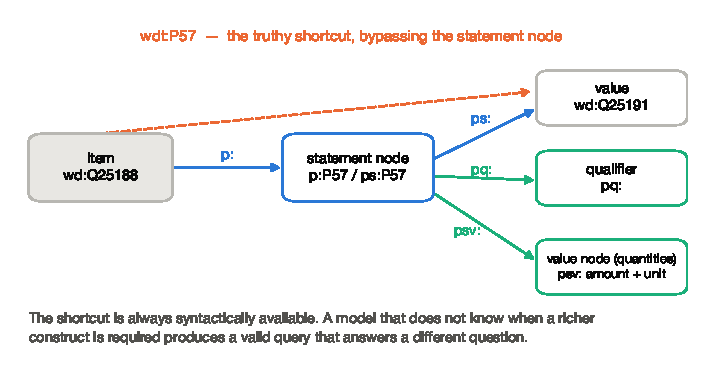
\includegraphics[width=0.88\textwidth]{figures/fig_wikidata_model.pdf}
  \caption{The Wikidata statement model.}
  \label{fig:wikidata-model}
  \tabnote{The truthy edge wdt: bypasses the statement node.
Qualifiers (pq:) and normalised value nodes (psv:) are reached
through p:/ps:.}
\end{figure}

\Cref{fig:wikidata-model} summarises these relationships.
One of them matters most here: the simpler query form is always syntactically available.
A model can use wdt: even when a statement node, qualifier or normalised value node is actually needed.
The resulting query is valid and may even return plausible results, yet it answers the wrong question.

Syntax checking cannot detect such an error; a comparison with the result of the gold query can.
Better entity linking cannot fix such an error either, because the identifiers are already correct.
For this reason, the thesis analyses structural and linking errors separately.

\subsection{SPARQL and Query Engines}

\label{sec:sparql}

SPARQL is the W3C query language for RDF, and the benchmark uses only part of it.
SPARQL matches graph patterns built from triple patterns and returns the variables selected in the SELECT clause.
The benchmark also uses FILTER for value constraints, OPTIONAL for left-join behaviour when a value may be missing, UNION for alternative patterns, aggregation with GROUP BY and HAVING, ordering and LIMIT, property paths such as the * and / operators described above, and subqueries.
Property paths matter for meaning, but they are also expensive to run.
Where they are placed and the order in which joins are evaluated can strongly affect execution time on a graph as large as Wikidata~\citep{aimonier2023joinordering}.

Two further features are specific to the Wikidata deployment.
The label service (SERVICE wikibase:label) adds human-readable labels to the identifiers in query results, and most published Wikidata queries use it.
The mwapi service lets a query call the MediaWiki API during execution, for example for full-text search.

\paragraph{Blazegraph and QLever}

The benchmark's gold queries were written for the public Wikidata Query Service, which runs on Blazegraph.
The experiments use a dedicated QLever instance instead~\citep{bast2017qlever}.
The reasons are practical: a local endpoint avoids the rate limits and timeouts of the public service and makes it easier to run thousands of queries under controlled conditions.
It also keeps the graph from changing during the experiments.

The two engines are not fully interchangeable.
Blazegraph supports named subqueries (WITH \ldots{} AS), the geospatial service wikibase:around, the mwapi service and the ``gas'' graph-traversal services; QLever does not.
QLever also applies stricter rules to AS targets and so rejects some queries that Blazegraph accepts.
As a result, around 15\,\% of the benchmark's gold queries run only on Blazegraph and are excluded from the evaluation.
The method chapter describes this issue in detail and discusses engine choice as a threat to comparability.

Real-world query use offers another point of comparison.
\citet{malyshev2018getting} analysed Wikidata Query Service logs and found that real users rely heavily on the label service and basic graph patterns, while more complex constructs are rarer.
The same comparison is made here, using the larger and more recent query-log corpus released by \citet{walter2026wdql}.
WDBench~\citep{angles2022wdbench} is a complementary benchmark built directly from public Wikidata query logs.

\section{Text-to-SPARQL and KGQA}

\subsection{Knowledge Graph Question
Answering}

\label{sec:kgqa}

Knowledge graph question answering (KGQA) means answering natural-language questions with the help of a knowledge graph.
Current research falls broadly into two approaches.
Recent surveys of large language models and knowledge graphs draw a similar line~\citep{ma2025llmkg}, as does a systematic review of the wider KGQA architecture space~\citep{perevalov2024survey}.

\paragraph{Retrieval-based
answering} treats the graph as a source to retrieve information from.
Relevant triples or subgraphs are retrieved, turned into text and given to a language model, which writes the answer directly.
This approach copes fairly well with differences in graph schema and needs no knowledge of query syntax.
The answer, however, is generated rather than computed.
It cannot be audited directly or re-run when the graph changes, and it does not scale naturally to large numbers of entities.
A question that needs aggregation over thousands of entities, for instance, cannot usually be answered from a handful of retrieved triples.

\paragraph{Semantic parsing} translates the natural-language question into an executable SPARQL
query.
The answer then comes from executing the query on the graph.
This work uses semantic parsing, because the query is an artefact that can be inspected and verified, works over any number of entities, and stays useful as the graph is updated.
The price is brittleness: one wrong identifier or one missing * can yield a query that is valid but wrong.
The experiments here measure and attribute this kind of failure.

Within semantic parsing, three system paradigms recur:

\begin{description}
\item[Fine-tuned sequence-to-sequence models]
are trained on question--query pairs and generate a query in one pass.
\item[Pipelines]
divide the task into explicit stages, typically including mention detection, linking, query generation, and execution~\citep{banerjee2024diss}.
Each stage can use a separate component or prompt.
\item[Agents]
give a model tools for exploring the graph and iteratively modifying a query.
Execution results can be used as feedback across multiple turns.
\end{description}

This thesis uses a pipeline.
Fine-tuned models need in-domain training data, have to be retrained for every knowledge graph, and cannot be built on frontier models that are only available through an API.
Agents can recover from their own mistakes, but they make many model and endpoint calls per question, and because each step depends on the one before, it is hard to tell which step caused a failure.
A pipeline keeps every stage observable, so each error can be traced to a specific stage, which is the central aim of this thesis.

\subsection{Text-to-SPARQL with Language
Models}

\label{sec:related-t2s}

The following paragraphs cover fine-tuned models, prompting, in-context learning, and agents, followed by recent schema-aware grounding methods that can complement these approaches.

\paragraph{Fine-tuned sequence-to-sequence
models}

\citet{banerjee2022modern} establish Wikidata semantic-parsing baselines with pre-trained sequence-to-sequence models.
They supply entity and relation links instead of predicting them, so the evaluation isolates query generation, and general-purpose models turn out to compete with task-specific architectures once linking is fixed.
\citet{xu2023wikisp} fine-tune LLaMA and introduce WikiWebQuestions, attributing 35.1\,\% of failures to entity linking (``the biggest source of errors'') and 17.1\,\% to the wrong property.
That attribution is re-tested here under two conditions that differ from theirs: their percentages are computed over failed examples only, and their system is fine-tuned on relatively simple questions.
When the generator is a frozen frontier model and disambiguation is close to perfect, the remaining error looks different: structure dominates, and linking contributes little.

\paragraph{Prompting and in-context
learning}

\citet{dabramo2025investigating} study in-context learning for text-to-SPARQL on benchmarks that supply gold entities and relations (so their evaluation, like \citet{banerjee2022modern}'s, isolates generation), and identify a systematic \emph{triple-flip} error: the model reverses the subject and object of a generated triple, producing a query that is valid, incorrect and often empty.
Their fix keeps several beam-search hypotheses instead of only the most probable one.
This independently supports the distinction between linking and structure drawn here.
It also connects to the empty results observed in this work: a structurally wrong query over correct identifiers often returns nothing, so an empty result can be a diagnostic signal.
Few-shot demonstrations can also teach more than surface format: \citet{shah2024implicit} show that examples which make implicit multi-hop reasoning steps visible improve generated SPARQL and Cypher queries, a more targeted use of demonstrations than the few-shot condition tested here.

\paragraph{Agentic systems}

Agentic approaches let a model explore the graph and revise a query over several steps~\citep{liu2024spinach}.
The TEXT2SPARQL'25 challenge produced several such systems: mKGQAgent~\citep{perevalov2025mkgqagent} won overall with a multilingual pipeline modelled on human reasoning; \citet{brei2025aruqula} combine ReAct-style reasoning with graph-exploration tools; and \citet{walter2025grasp} extend the approach from one knowledge graph to many.
\citet{soru2026researcher}'s self-improving agent reaches 0.22 accuracy on the 2025 DBpedia validation set and concludes that ``the bottleneck is consistently in basic-graph-pattern predicate selection, not in SPARQL syntax or modifiers''.
On a different graph and system, this supports the failure taxonomy of this work.
These systems share execution-guided revision, and the cascade used here is a deliberately minimal form of it.

\paragraph{Schema-aware grounding}

\citet{zhang2026saga}'s SAGA keeps a persistent bidirectional type state and filters candidate properties by entity type, property domain/range and expected answer type, reporting the highest F1 across nine Wikidata/Freebase settings and fewer empty results.
In other words, SAGA removes unsuitable candidates before generation.
The schema-evidence prompt tested in this work only adds schema information to the prompt as text, which the generator is free to ignore, and in the experiments here it did not improve accuracy.
The discussion chapter explains why this difference, filtering the candidate space rather than merely informing it, matters.
\citet{yang2026ggc}'s Generator--Gate--Corrector applies correction only to the questions that need it and cuts inference overhead by 45\,\%.
The selective-application experiment in this work tests the same gating idea for a different intervention and finds that it does not beat applying the intervention everywhere.
\citet{srivastava2026mars} use adaptive multi-hop retrieval that learns when to stop traversing the graph and start generating, with competitive results on three multilingual KGQA benchmarks.
Recent production-oriented systems organise text-to-SPARQL in the same way, as a pipeline of metadata indexing, prompt construction, generation and execution, which shows how much grounding and endpoint interaction matter beyond one-shot query decoding~\citep{smeros2025sparqlllm}.

\section{Entity Linking for KGQA}

\subsection{Entity Linking}

\label{sec:el-background}

Entity linking maps textual mentions to identifiers in a knowledge base.
\citet{shen2015entitylinking} describe the standard three stages: \emph{mention detection}, which finds the spans to be linked; \emph{candidate generation}, which retrieves a shortlist of possible identifiers for each mention, usually from an alias index; and \emph{candidate ranking}.
\citet{moller2022survey} show that Wikidata entity linking is shaped by conditions that ordinary systems for encyclopaedic text make little use of: a multilingual and constantly changing space of labels and aliases, a long tail of non-named entities, and the hyper-relational statement model described above, which carries more information than a plain named-entity mention.
The linking results later in the thesis should be read with this last point in mind.

\paragraph{Linking for a query is not linking in
text.}

A classic entity linker finds references to named entities in a document and connects them to knowledge-base identifiers.
It is built for running text.
A text-to-SPARQL pipeline needs something different, because a query may require identifiers for relations (P57, director), type constraints (Q5, human), units and aggregation concepts.
Many of these never appear as named entities in the question.
“How many female directors won an Oscar after 2000?” may require identifiers for instance of, human, sex or gender, female, award received and director, although several of these concepts are not explicit spans in the text.
A linker that starts from mention detection in the text cannot find a concept the question does not state.
This is a mismatch between the task these systems were built for and the task they face here, not necessarily a flaw in their implementation.
It helps explain the large differences in the linker comparison between text-driven end-to-end linkers and approaches that reason over candidates retrieved for the vocabulary a query needs.
These results should not be read as a general judgement on end-to-end linking systems.

\subsection{Entity Linking Paradigms}

\label{sec:related-linking}

The following three paradigms correspond to the linking approaches evaluated here.
The section closes with how linkers should be evaluated so that they can be compared fairly.

\paragraph{Fine-tuned end-to-end
linking}

\citet{wu2020blink} introduced BLINK, a two-stage architecture in which a bi-encoder retrieves candidates by dense vector similarity and a cross-encoder re-ranks them.
It is trained on Wikipedia hyperlinks and transfers zero-shot to unseen entities.
\citet{li2020elq} adapt this approach to questions with ELQ, which detects and links mentions in a single pass over the question, with efficiency as a central design goal.
\citet{ayoola2022refined} propose ReFinED, which performs mention detection, fine-grained typing and disambiguation in one pass over a document and scales to the full Wikidata entity set.

All three systems are trained on running text and detect mentions in that text.
As discussed above, this is not the same as supplying the broader vocabulary a SPARQL query needs, and their results in the linker comparison should be read with this mismatch in mind.

\paragraph{Zero-shot bi-encoder
retrieval}

GLiNER is a lightweight named-entity recognition model that compares text spans with descriptions of entity types, so it can recognise types it was not trained on.
\citet{stepanov2026glinker} extend its bi-encoder variant to large label spaces and introduce GLiNKER as an entity-linking framework.
Its main advantages here are that it needs no task-specific training and scales to Wikidata's large label space.
Its drawback is typical of bi-encoders: the mention and each candidate are encoded separately, which makes retrieval fast but rules out a detailed comparison between them, so similar candidates are harder to tell apart than when they are ranked jointly with the question.

\paragraph{Reasoning over retrieved
candidates}

The third paradigm retrieves candidates from an alias index and asks a language model to choose among them, using the question as context.
\citet{alekseev2025querybased} evaluate this approach inside a multi-stage Wikidata pipeline.
They compare reasoning-based selection with fine-tuned linking and argue for query-based KGQA on complex and temporal questions.
Theirs is the published work closest to the pipeline evaluated here, and the end of this chapter positions this thesis against it explicitly.

\citet{vollmers2025evaluation} evaluate entity and relation linking specifically for KGQA.
They report that linkers based on language models clearly outperform other approaches, especially in recall.
In their comparison, traditional systems reach higher precision but much lower recall.
They also draw a conclusion that bears directly on the design used here: high recall, even at some cost in precision, can give better end-to-end performance, because the downstream model tolerates noisy candidate sets.

The same pattern appears here, on a different benchmark and with differently constructed ground truth.
It also explains the candidate-pool design used here: retrieval deliberately admits candidates generously, and the disambiguation stage is responsible for choosing the right one with the full question as context.

\paragraph{Evaluation protocol}

\citet{bast2023fairel} point out that published end-to-end entity-linking results are often hard to compare, because systems differ in what they count as a mention, how they score partial overlaps and which knowledge-base version they use.
They propose an evaluation framework that controls these choices.
The linking comparison here follows the same discipline: all four linkers are evaluated on identical rows, against identical ground truth, with identical scoring.
The ground truth comes from the benchmark's own annotated queries, not from an external linker's index.

\section{Benchmarks, Evaluation, and Research
Gap}

\subsection{Benchmarks and Evaluation
Practice}

\label{sec:related-eval}

\paragraph{The benchmark used here}

\citet{benamor2025instruct} introduce Instruct-to-SPARQL, built by crawling Wikidata tutorial and example pages and pairing the queries found there with generated instructions and complexity labels.
Two of its properties matter here.
Because it comes from documentation and community examples rather than templates, it contains a wide range of Wikidata-specific idioms (qualifiers, statement nodes, the label service), which suits a study of structural competence.
And, as the authors state, it comes with no entity-linking strategy, leaving grounding to the system.
\citet{dubey2019lcquad2} remains one of the most widely used Wikidata KGQA benchmarks and offers a point of comparison for scale and construction.

\paragraph{The comparability problem}

Published text-to-SPARQL results are hard to compare directly: studies use different graph snapshots, metrics that share a name but not a definition, and gold queries that may no longer execute.
This is part of a wider benchmark-design problem in KGQA: datasets differ in how they construct questions, annotate logical forms and define complexity, so reported improvements may not carry over to other benchmarks or graph snapshots~\citep{steinmetz2021kgqabenchmarks}.
\citet{taghzouti2026t2smetrics} document this fragmentation and propose a unified evaluation library, which itself shows that consistency is still an open issue.
For this reason, the benchmark authors' generated queries are re-executed here against the same snapshot, fair-set definition and metric as every other system, and published scores are not compared directly.

\paragraph{Contamination and
memorisation}

A model that saw a benchmark's gold queries during pre-training may partly reproduce them from memory.
\citet{gashkov2025memorization} show that this can affect reported performance on QALD and LC-QuAD.
Instead of assuming that the frozen frontier models are or are not contaminated, this work measures the effect directly.
Identifiers, literals and variable names are removed from every generated query, and the remaining structure is compared with the benchmark's reference queries.
A model that had memorised the benchmark would often reproduce them almost exactly.

\paragraph{External validity}

A benchmark's mix of constructs does not necessarily reflect what users actually ask.
\citet{malyshev2018getting} established the practice of comparing benchmark constructs with Wikidata Query Service logs, and \citet{walter2026wdql} released a much larger derived resource of 335,000 question--query pairs for the same purpose.
It is used here to check whether the Wikidata idioms under study are a property of the benchmark or of real-world use.

\subsection{Positioning of This Work}

\label{sec:positioning}

\paragraph{Established components}

The pipeline builds on two established mechanisms: reasoning-based disambiguation over retrieved candidates, studied by \citet{alekseev2025querybased} (who compare it with fine-tuned linking in a multi-stage Wikidata pipeline) and \citet{vollmers2025evaluation}; and execution-guided revision, established in the agentic systems discussed above.
The cascade used here is a minimal, single-round form of execution feedback, added because the measurements showed remaining headroom.

\paragraph{What differs here}

The linking comparison evaluates four paradigms on the same rows, ground truth and candidate pools, with the gold standard taken from the benchmark's own annotated queries.
Error is attributed to individual stages, with backbone dependence measured separately for each, instead of being reduced to one end-to-end score.
Interventions are controlled by changing only the generation prompt, and four directions are tested: generic guidance, schema evidence, selective guidance and a closed vocabulary.
External validity is checked against real query-log usage in both directions.

\paragraph{Framing}

The contribution is primarily measurement and attribution: finding where a frozen-model pipeline fails, identifying which component is the main constraint, and introducing one mechanism that follows directly from that evidence.

\chapter{Research Design and Method}

\label{ch:method}

This chapter describes what was built, what it was tested on and how it was evaluated.
It covers the evaluation method, the pipeline, the benchmark and its two splits, four linking methods, the linking ground truth, the execution environment and metrics, the prompt interventions, the recovery methods, and the models and reproducibility procedures.

\section{Stage-Wise Diagnostic
Evaluation}

Text-to-SPARQL systems are usually evaluated end to end, with one score per system that shows how useful it is but says little about why it fails: one system may identify every entity correctly but build the wrong structure, another may get the structure right but use a wrong identifier, and both end up with the same score for different reasons.
The underlying process can nonetheless be split into component decisions (entity detection, entity linking, relation selection and query construction)~\citep{mohammed2018strong}, and this is what makes stage-wise measurement possible.

This thesis uses stage-wise diagnostic evaluation, a four-step protocol (\cref{fig:method}).

\textbf{First, intermediate ground truth is derived from artefacts the benchmark already provides.}
Instruct-to-SPARQL contains each query twice, once with identifiers and once with those identifiers replaced by labels; since the two versions are aligned position by position, they yield mention-level linking ground truth without additional annotation, and the same approach works for any benchmark that provides aligned gold and label-form queries.

\textbf{Second, the stage of interest is isolated by keeping all other stages fixed.}
Each condition changes only one component and reuses the same generated queries, candidate pools, execution environment and scoring; where possible, the varied stage also receives its gold value, which creates an upper-bound condition (not itself a performance claim) whose difference from the full pipeline estimates the error attributable to that stage.

\textbf{Third, the remaining error is attributed and checked against independent evidence.}
Simple subtraction is not enough, because the unexplained remainder may have several causes, so the subtraction-based attribution is compared with a manually annotated failure sample, corpus-wide construct counts and agreement between independent systems; the attribution is reported with the confidence interval that the weakest evidence supports, and disagreements between sources are reported as well.

\textbf{Fourth, the proposed cause is tested through intervention.}
If a system lacks particular knowledge, supplying it should improve performance, and the size of the improvement shows how much error the missing knowledge explains.
Interventions that do not help are still informative, because they narrow down the explanations for the observed errors; the next chapter reports all of them alongside the one that works.

The protocol is defined independently of the specific pipeline used here.

\begin{figure}[htbp]
  \centering
  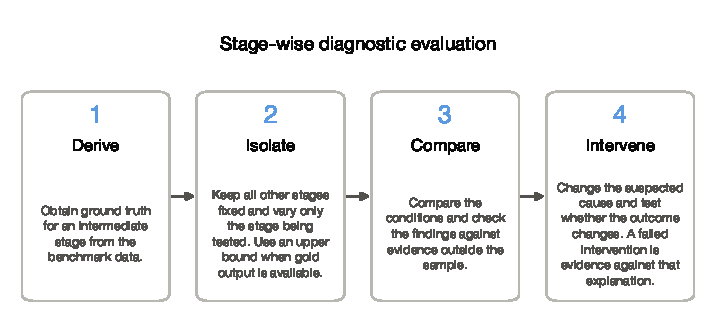
\includegraphics[width=0.88\textwidth]{figures/fig_method.pdf}
  \caption{\Method{}: the four moves.}
  \label{fig:method}
  \tabnote{The protocol is independent of the pipeline and can
be applied to other benchmarks that provide aligned gold and label-form
queries.}
\end{figure}

\section{Pipeline Architecture}

\label{sec:method-framework}

The system is a modular pipeline built on frozen language models, and no stage uses fine-tuning.
It follows the pipeline paradigm described in the previous chapter, with fixed stages and observable intermediate outputs instead of a single sequence-to-sequence model or an open-ended agent.
This design was chosen mainly with diagnosis in mind: named stages can be measured, replaced and given gold values one at a time, as the diagnostic protocol requires.

\paragraph{The Six Stages}

For each question, the pipeline runs the following steps.
\Cref{fig:pipeline} shows the complete arrangement and the two evaluation conditions.

\textbf{1.\ Labelled-query generation.}
The model receives a system prompt that asks it to act as a Wikidata SPARQL expert and write a query that answers the question.
Instead of opaque identifiers, it must use human-readable labels in a fixed bracket format: wd:[entity:LABEL] for entities and wdt:[property:LABEL] for properties.
It is told to keep ordinary SPARQL structure and to output only the query.
Decoding is deterministic, and Markdown code fences are removed.
The notation comes from the benchmark itself.
\textcite{xu2023wikisp} use a similar label-based representation, as do \textcite{banerjee2023gettqa}, whose grounding step based on graph embeddings performs a comparable substitution from labels to identifiers.
Using the benchmark's notation means that generated and reference queries can be compared in the same vocabulary.

\textbf{2.\ Label parsing.}
Regular expressions extract the entity and property labels from the generated query.
Duplicate labels are removed, and the original order is kept.

\textbf{3.\ Candidate retrieval.}
For each label, the top seven candidates are retrieved from Wikidata's wbsearchentities API.
Entity labels are searched among items and property labels among properties.
Each candidate comes with an identifier, a label and a short description.

When requests arrive too quickly, the API can silently return empty results, which makes throttling hard to tell apart from a label that has no matching candidate.
To reduce this problem, requests are rate-limited and candidate pools combine repeated retrievals.
Empty results are requested again until the pools are stable.

\textbf{4.\ Disambiguation.}
Each label is mapped to one candidate identifier.
This is the stage that the linker comparison varies, and the four implementations are described below.
All other stages stay the same, so the comparison concentrates on the disambiguation mechanisms.

\textbf{5.\ Substitution.}
The selected identifiers replace the labels in the query.
A query counts as fully linked only when no bracket placeholder remains.
Partial substitution is recorded as a linking failure and is not passed on to execution.

\textbf{6.\ Execution and scoring.}
The substituted query is executed against the endpoint, and its result set is compared with the reference result set.
The execution environment and the scoring metric are described later in this chapter.
For each question, the pipeline records whether a labelled query was generated, whether all labels were linked and whether the query executed.
These indicators make the stage analysis in the results chapter possible.

\paragraph{Three Decisions}

Translating a question into a query involves three decisions.
\emph{Concept selection} decides which entities and properties the query needs.
\emph{Structural composition} arranges them with Wikidata's constructs, such as statement nodes, qualifiers, class closure and aggregation.
\emph{Disambiguation} decides which identifier a given label denotes, among the retrieved candidates.
In this pipeline the generator makes the first two decisions when it writes the labelled query, and the linking stage makes the third.
In this thesis, \emph{linking} refers to the third decision, the mapping from a label to its identifier.

\paragraph{Two Conditions}

The pipeline is evaluated under two conditions, and the difference between them is the upper-bound construction described above.

In the \textbf{gold-label condition}, generation is skipped and the labels come from the benchmark's annotated query.
Concept selection and query structure are therefore correct by construction, and only disambiguation is evaluated.
Comparing this condition with the full pipeline estimates the error caused by generating the query, that is, by concept selection and structural composition together.

In the \textbf{end-to-end condition}, the model generates the labelled query and the same linking stages follow.
This condition represents the deployed system and provides the main pipeline results.

One design asymmetry needs mentioning.
Property labels are resolved with the reasoning-based method in every condition, including those in which other linkers resolve the entities, because none of the compared systems links Wikidata properties.
As a side benefit, entity-linking and property-linking errors can be measured separately, in line with \textcite{scharpf2026survey}, who identify joint entity and predicate linking as an underdeveloped area.
The split is a diagnostic design choice, not a claim that the two tasks are best solved independently: joint entity--relation linking is an established alternative that exploits the compatibility between candidate entities and relations~\citep{dubey2018earl}.

\begin{figure}[htbp]
  \centering
  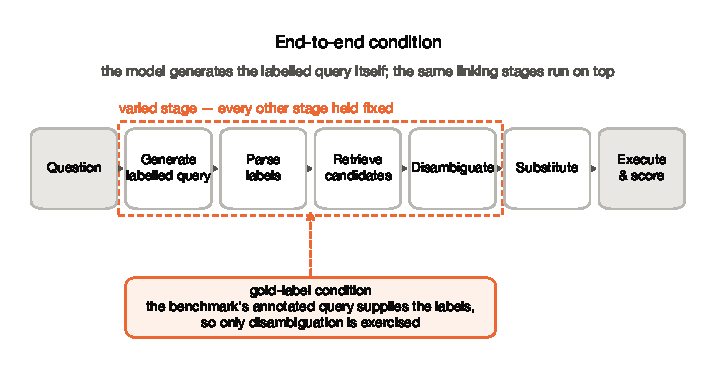
\includegraphics[width=0.88\textwidth]{figures/fig_pipeline.pdf}
  \caption{Pipeline architecture and the two evaluation conditions.}
  \label{fig:pipeline}
  \tabnote{The pipeline has six stages. In the gold-label
condition, the benchmark's annotated query supplies the labels, so
generation is skipped. All other stages remain identical.}
\end{figure}

\section{Benchmark and Experimental
Conditions}

\label{sec:method-pipeline}
\label{sec:setup-benchmark}

The benchmark is Instruct-to-SPARQL~\parencite{benamor2025instruct}.
It pairs natural-language instructions with executable Wikidata queries and assigns complexity labels.
It was chosen for three reasons.
First, its queries were collected from tutorial and example pages instead of being generated from templates, so they reflect the modelling conventions of actual Wikidata users.
Second, its complexity labels make it possible to see where systems fail.
Third, and most important here, each query is provided both with identifiers and with those identifiers replaced by human-readable labels, which enables the ground-truth derivation described below.

\paragraph{Two Splits, Two Jobs}

Two evaluation splits serve different purposes.
The \textbf{working split} was created from the released data with complexity stratification, a fixed seed and a 75/5/20 train-validation-test division, keeping one natural-language instruction per query.
Its test set contains 567 queries (38 simple, 222 medium, 307 complex) and is used for the diagnostic analysis: the stage table, error taxonomy, construct analysis, prompt interventions and cascade.
The \textbf{official split} is the benchmark authors' own test split, used for the comparison with their published systems.
Each experiment uses the split that fits its purpose and no result is reported twice, with one exception: the linker comparison is replicated on both splits to test whether it depends on the split chosen; differences in row counts are explained where they occur.

\begin{figure}[htbp]
  \centering
  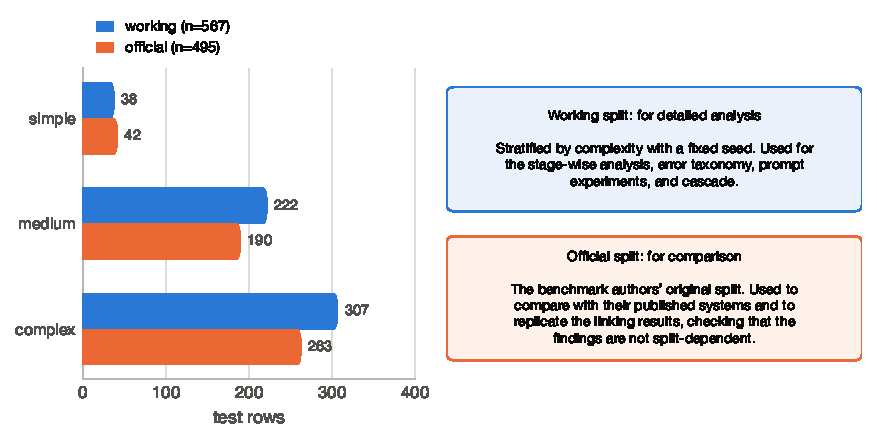
\includegraphics[width=0.88\textwidth]{figures/fig_splits.pdf}
  \caption{The two-split design.}
  \label{fig:splits}
  \tabnote{The splits have different purposes and are not
interchangeable. Only the linker comparison uses both splits, allowing
the stability of its ordering to be examined.}
\end{figure}

\paragraph{Dataset Drift}

The dataset's identifier field is not stable between the raw file used to build the working split and the current release.
Some identifiers point to different questions in the two versions, so rows are matched on normalised instruction text instead.
The release offers two configurations with different splits; the official-split experiments use the default configuration, whose 495 test rows match the benchmark paper (the with-limit configuration has 493).
Against the default configuration, 365 of the 567 working test rows (64.4\%) correspond to official training rows, 95 (16.8\%) to official test rows and 24 (4.2\%) to validation rows, 6 (1.1\%) have instructions that occur in more than one official split, and 77 (13.6\%) have no counterpart; the revision used here is pinned in the repository.
This overlap does not contaminate the results of this thesis, since none of the models is fine-tuned on the benchmark; it matters only for the comparison with the authors' fine-tuned systems, which is why that comparison uses the official split.

\section{Linking Methods and Ground
Truth}

\subsection{Linker Implementations}

\label{sec:method-linkers}

Four implementations are used in the disambiguation stage.
They represent different paradigms from the entity-linking literature and are inserted at the same point in the pipeline.

\paragraph{Reasoning over Retrieved
Candidates}

A language model receives the label, the question and the retrieved candidate list, in which each candidate has an identifier, a label and a description.
It is asked to reason about which candidate best matches the label in the context of the question and to output the chosen identifier in a fixed format.
Decoding is deterministic.
If only one candidate is retrieved, it is selected without a model call.
If no identifier can be extracted from the response, the top search result is used as a fallback.

This approach follows RetReason in \textcite{alekseev2025querybased}; this thesis compares it with the other paradigms under identical conditions and across backbones of different sizes and origins.
Three backbones are used: Claude Opus 4.8, Qwen2.5-14B-Instruct, and Qwen2.5-7B-Instruct.
The two open-weight models run on the AI \& Explainability group's GPU server.
The prompt, candidate pools, reference and evaluator stay fixed, so the backbone is the only variable that changes.
On the official split, the reasoning linker is run with Qwen2.5-14B-Instruct only: the open-weight models were available on the group's GPU server, whereas Claude Opus 4.8 is accessed through a paid API, so its use was limited to the working split to keep costs manageable.

\paragraph{Zero-Shot Bi-Encoder
Retrieval}

GLiNKER~\parencite{stepanov2026glinker} is a modular entity-linking framework based on the GLiNER bi-encoder architecture.
It is used in external-mentions mode with gliner-linker-large-v1.0.
Each label extracted from the query is supplied as a mention span, embedded in the question as context, and GLiNKER chooses among the same seven candidates the reasoning linker receives, each given by its label and description.
The candidates are passed to it directly, because its default entity store looks a mention up by exact label and keeps one entity per label, which would show it at most one candidate.

Using the same candidates as the reasoning-based linker isolates the disambiguation mechanism.
It does not, however, test GLiNKER the way its authors intended, since the framework is designed to retrieve from large entity databases with its own multi-stage retrieval.
Its score therefore measures one mechanism inside this pipeline, not the framework as a whole.
The discussion returns to this limitation.

\paragraph{Fine-Tuned End-to-End
Linking}

Two systems represent the fine-tuned paradigm.

ReFinED~\parencite{ayoola2022refined} performs mention detection, fine-grained typing and disambiguation in one forward pass.
It is run with the questions\_model checkpoint against the complete Wikidata entity set.
\textcite{xu2023wikisp} and \textcite{alekseev2025querybased} also used ReFinED, which makes the results comparable with related work.

ELQ~\parencite{li2020elq}, the question-focused version of BLINK~\parencite{wu2020blink}, detects mentions and links them jointly in one pass, using an entity library derived from Wikipedia.
It was run on the group's GPU server.
Vanilla BLINK was not evaluated separately: ELQ is its question-oriented variant from the same repository and uses an entity library of the same 2019 Wikipedia snapshot, so it represents this family for questions.

Unlike the first two implementations, ReFinED and ELQ detect mentions in the question themselves instead of receiving the labels extracted from the generated query.
This is part of the paradigm under evaluation, but it means the four systems do not solve exactly the same sub-task.
The set-based metric described below reduces this alignment penalty and estimates how much of the deficit comes from mention detection rather than disambiguation.

\paragraph{What Is Held Constant}

Across all four implementations, the evaluated rows, reference identifiers, candidate pools (where they apply), substitution and execution procedures, and scoring code are identical.
Only the disambiguation mechanism changes.
This is what makes the linker comparison sound, and it avoids the problems of comparing published scores obtained on different corpora, metrics and knowledge-graph snapshots.

\subsection{Linking Ground Truth}

\label{sec:setup-groundtruth}

The benchmark does not annotate linking outputs directly.
The reference can, however, be derived from the aligned query forms, following the first step of the diagnostic protocol.

\paragraph{Derivation}

The annotated query differs from the reference query only in that identifiers are replaced by bracketed labels.
The $i$-th label in the annotated query therefore corresponds to the $i$-th identifier in the reference query, and walking through both forms in parallel recovers each label--identifier pair.
The label type is checked against the identifier type: an entity label must align with a Q identifier and a property label with a P identifier, so alignment errors cannot slip through unnoticed.
\Cref{fig:groundtruth} gives an example.

On the working split, alignment succeeds for 547 of 567 rows (96.5\%), producing 1,086 entity mentions and 2,766 property mentions.
On the official split, it succeeds for 472 rows, producing 1,055 entity mentions and 2,271 property mentions.
Rows in which the numbers of labels and identifiers differ are excluded from the linking evaluation for every linker, so the excluded rows do not affect the comparison.

The method requires aligned gold and label-form queries, but no new annotation, external linker index or assumption about which entities appear in the question.
Many reference identifiers stand for classes or units that the question never mentions explicitly, so this independence from the question text is essential.

\paragraph{Candidate Ceiling}

Two of the linking implementations choose from a shared candidate pool.
They cannot recover an identifier that is missing from that pool, so candidate coverage has to be checked before their scores can be interpreted.

With the rate-limited retrieval described above, the reference identifier is present for 1,080 of 1,086 entity mentions (99.4\%) and 2,730 of 2,766 property mentions (98.7\%).
Candidate retrieval is therefore not a binding constraint in the comparison.

\begin{figure}[htbp]
  \centering
  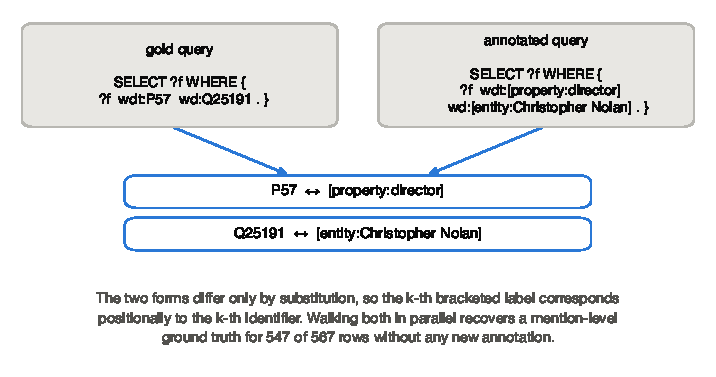
\includegraphics[width=0.88\textwidth]{figures/fig_groundtruth.pdf}
  \caption{Deriving mention-level linking ground truth from the benchmark.}
  \label{fig:groundtruth}
  \tabnote{Since the annotated query differs from the gold
query only through identifier substitution, alignment is positional and
requires no new annotation. It succeeds on 547 of 567 rows. The 20 rows
with different bracket and identifier counts are excluded for every
linker.}
\end{figure}

\section{Evaluation and Execution}

\subsection{Execution Environment}

\label{sec:setup-endpoint}

All queries are executed against a QLever instance provided by the AI \& Explainability group, indexing a Wikidata snapshot dated 14 March 2026; it was chosen because the rate limits and timeouts of the public Wikidata Query Service lowered execution success for reasons unrelated to query quality.
Three adaptations apply equally to reference and generated queries: the standard prefix block is added (QLever does not define it implicitly), \texttt{SERVICE wikibase:label} clauses are removed (they are Blazegraph-specific and affect only display labels, not the identifiers used for scoring), and responses are streamed with a 50 MB limit, above which they count as failures.
Execution failures are classified by cause (HTTP status, timeout, connection error, oversized result), as the stage analysis requires.

\paragraph{The Exclusion Taxonomy}

Of the 567 working test rows, 111 reference queries do not execute on QLever.
Of these, 26 also fail on the public endpoint (knowledge-graph evolution), and the remaining 85 fail for engine-specific reasons: Blazegraph's proprietary named-subquery extension, unavailable services (\texttt{wikibase:around}, \texttt{mwapi}, \texttt{gas}), timeouts, and queries that reuse a variable as an \texttt{AS} target (which QLever rejects as non-standard SPARQL while Blazegraph accepts it).
Approximately 15\,\% of reference queries are therefore Blazegraph-only; since generated queries face the same constraints, this does not bias the comparison between systems, but the evaluated subset is not a uniform sample of the full benchmark (see the limitations).

\subsection{Evaluation Metrics}

\label{sec:setup-metrics}

\paragraph{Result-Set Similarity and the Empty-Set
Artefact}

Accuracy is measured as the Jaccard similarity between the generated and reference result sets, after entity URIs are normalised to identifiers.
Two evaluation sets are used: the lenient set (456 of 567 working rows, wherever the reference executes) and the strict set, which additionally requires the reference to return at least one result (400 rows: 35 simple, 194 medium, 171 complex; these are \emph{scorable} counts, not the split's composition given above).
All headline results use the strict set.
It removes the first of the four metric problems examined in the discussion: the Jaccard similarity of two empty sets is 1.0, so among the 56 rows where the reference executes but returns nothing, a wrong generated query that also returned nothing scored perfectly, which inflated scores by two to seven points and changed model rankings in preliminary experiments.

\paragraph{Entity-Level Similarity as a Robustness
Check}

The pooled metric combines values across all result columns, so label mismatches lower it even when the underlying entities agree (about 16\,\% of end-to-end rows).
Entity-level Jaccard, which uses only identifiers, is therefore reported as well; it is up to six points higher and leaves the system ordering unchanged, which suggests that the pooled metric understates but does not distort the comparisons.
It is undefined when neither query returns entity values, so comparisons use the 316 strict rows where it is defined for every system (27 simple, 166 medium, 123 complex); full-set results are in the appendix.

\paragraph{Linking Metrics}

Linking is evaluated directly, because a query can fail structurally with every identifier correct, and one wrong identifier can spoil an otherwise correct query.
For each linker, precision, recall and F1 are computed over the predicted identifiers at mention level (exact match only; an unresolved mention counts against recall, not precision), together with the proportion of fully linked queries, broken down by complexity.
For ReFinED and ELQ, set-based precision, recall and F1 are computed as well (predicted versus reference identifier sets, without mention-level alignment), so the gap between mention-level and set-based scores estimates the effect of mention detection separately from disambiguation.

\paragraph{Construct-Agreement F1}

Usage counts alone cannot tell apart a system that never uses a construct from one that uses it constantly in the wrong places, and only the second is a calibration problem.
Construct-agreement F1 separates the two: with ``the reference query for question $q$ uses construct $C$'' as the positive class, it is the per-question F1 with which a system uses $C$ exactly where the reference does.
Because it is computed over query text rather than answers, knowledge-graph evolution does not affect it, and it stays meaningful even for rows whose reference no longer executes.

\paragraph{Statistical Testing}

Paired comparisons are reported with confidence intervals.
Prompt interventions and the cascade use paired bootstrap percentile intervals, a two-sided permutation test and the Wilcoxon signed-rank test; the linker comparison uses mention-level bootstrap resampling, applying the same resample to every linker in each iteration.
Complexity breakdowns and the comparison with the benchmark authors' systems are point estimates; differences below about one percentage point between neighbouring configurations are treated as ties, and the 27-row simple category in the common entity-level subset should be read with caution.

\section{Interventions and Failure
Recovery}

\subsection{Prompt Interventions}

\label{sec:method-prompts}

The error analysis in the results chapter identifies query structure as the main source of failure, in particular the underuse of constructs for qualified, quantified and hierarchical facts.
If this explanation is right, giving the model information about these constructs should improve generation.
Four prompt conditions test this.

All conditions use the same model, candidate pools, disambiguation backbone, execution environment and scoring; only the generation prompt changes.

\paragraph{Baseline.}

The model receives the task description given above: generate a query in bracket notation, keep ordinary SPARQL structure, and output only the query.

\paragraph{Idiom guidance.}

The baseline prompt is extended with seven rules about Wikidata modelling patterns.
They cover hierarchical class membership, statement nodes and qualifiers, value nodes for quantities, lexemes and forms, aggregation for counting and ranking, VALUES or UNION for alternatives, and avoiding unnecessary LIMIT clauses.
The model is told to apply only the constructs the question requires.
Each rule addresses a failure mode found in the error analysis, and the complete prompt is given in the appendix.

\paragraph{Schema evidence, verbose and
targeted.}

Generic guidance explains that a construct exists; schema evidence gives information about the entities and properties relevant to a specific question.
Following~\parencite{zhang2026saga}, the reference identifiers are probed against the endpoint to find their properties, qualifiers, class relationships and quantity values.
The information is presented in two forms:

\begin{itemize}
\item
A verbose card listing all retrieved information, averaging 329 words.
\item
A targeted card with conditional guidance for properties relevant to the question.

\end{itemize}

The cards are built from reference-linked mentions, not from the mentions the pipeline resolves.
This favours grounding, but the setting is not deployable because it relies on gold information, so it is treated as an upper-bound condition in the sense of the diagnostic protocol.

\subsection{Selective Application and the Execution-Guided
Cascade}

\label{sec:method-cascade}

The interventions raise a further question: can guidance be given only when it is needed?

\paragraph{Selective Application}

Unconditional idiom guidance can lead the model to overuse the constructs it describes.
A selective gate could predict whether a question needs a particular construct and include the matching rule only then, an approach also suggested by~\parencite{yang2026ggc}.

Such a gate must meet two conditions: the need for a construct must be predictable from the question, and the guidance must do harm when the construct is not needed.

To test predictability, a logistic-regression classifier is trained on unigram and bigram term-frequency features from the training split, with labels indicating whether the reference query uses the construct.
To test whether selective application could help, the effect of idiom guidance is measured separately for questions that do and do not need each construct.
An oracle gate then applies guidance only when the reference query requires a reification or hierarchy construct.
Because the oracle has access to the reference query, it represents the best possible gate, not a deployable system.

\paragraph{The Execution-Guided
Cascade}

The cascade relies on an observable failure signal instead of predicting the cause directly.
Every reference query in the evaluation set returns at least one result, so a generated query that executes but returns nothing must be wrong.

The cascade generates several queries for the same question with different prompts.
It executes them in a fixed order and accepts the first result set that is non-empty and free of execution errors (\cref{fig:cascade-mechanism}).

On this evaluation set, the method is monotonic.
It only replaces empty or failed results, which already score zero against a non-empty reference.
It needs no gold answers and no training.
A question whose first query fails is passed to the next prompt in the order, so it costs one further generation per fallback step; with the eight runs reported here, at most seven.

\begin{figure}[htbp]
  \centering
  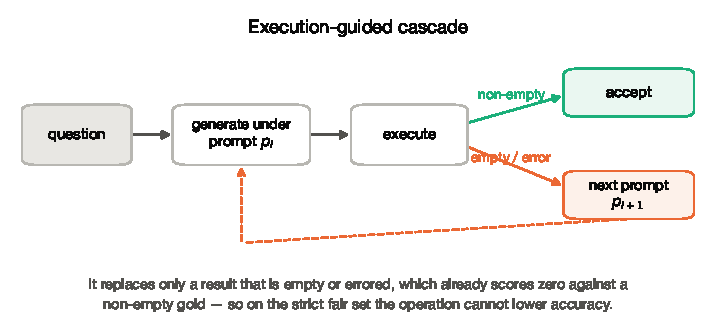
\includegraphics[width=0.88\textwidth]{figures/fig_cascade_mechanism.pdf}
  \caption{The execution-guided cascade.}
  \label{fig:cascade-mechanism}
  \tabnote{The trigger is similar to the execution feedback used by
agentic systems, but the cascade responds with a different prompt rather
than an open-ended self-correction loop. This limits the cost and
ensures monotonicity.}
\end{figure}

The cascade is compared with two alternatives that use the same candidates.
The first selects a result-set centroid: among the candidates that return results, it picks the one whose result set is, on average, most similar to the others.
The second adds a fallback to the best-performing single prompt when no candidates agree above a threshold.
These comparisons show whether the useful signal comes from agreement between candidate answers or simply from having a valid preferred result.

Execution feedback is established in mKGQAgent~\parencite{perevalov2025mkgqagent}, SPINACH~\parencite{liu2024spinach}, and GRASP~\parencite{walter2025grasp}.
These systems generally send execution failures back to the same prompt for revision.
A recent reinforcement-learning agent learns a policy for this revision step directly, training a compact model to recover from execution errors across turns~\parencite{vossebeld2025refine}.
The cascade instead switches to a different prompt for the same question, which limits the number of calls and makes it monotonic.

\section{Models and
Reproducibility}

\label{sec:setup-repro}

\paragraph{Models}

Four frozen frontier models are evaluated for generation: GPT-5.4, Claude Opus 4.8, Gemini 3.1 Flash Lite, and DeepSeek V4 Flash, accessed through the OpenRouter API with deterministic decoding, a 1,024-token limit, and up to three retries on empty responses.
The prompt-intervention arms, the official-split comparison and the Claude Opus 5 replication were run directly through Anthropic's API.
In the pipeline, Claude Opus 4.8 generates the labelled queries, except in the newer-model replication, which uses Claude Opus 5.
Claude Opus 4.8 also disambiguates in the working-split end-to-end run; the official-split run, the prompt-intervention arms and the Opus 5 replication disambiguate with Qwen2.5-14B-Instruct, and the backbone comparison varies the disambiguation model.
Qwen2.5-14B-Instruct and Qwen2.5-7B-Instruct are served through vLLM on the AI \& Explainability group's GPU server.

The seven prompt-intervention arms use Claude Opus 4.8 for generation and the same open-weight disambiguation model throughout, so the prompt is the only experimental variable.
This configuration was chosen because the experiment required seven complete pipeline runs, and it is supported by the backbone comparison, which shows similar disambiguation performance across backbones (97.7 entity F1 frontier vs.\ 94.9 and 95.8 open).
Absolute scores in these arms are therefore slightly lower than the frontier-disambiguated end-to-end results; comparisons within the arms remain valid, but absolute scores across sections should be read with this in mind.
The generator's identity was checked between arms through its lexical fingerprint (camelCase identifiers, snake\_case labels, bare property identifiers): all seven arms pass, while an open-backbone control run fails, which confirms that the check can detect a changed generator.

The official-split comparison differs in two respects: it uses Anthropic's batch interface, and it sets no temperature, since the API no longer supports this parameter for the model.
The two experiment sets should therefore not be compared at sub-percentage-point precision.

\paragraph{Caching, Re-Scoring, and Reproducibility}

Model outputs (generated queries, disambiguation decisions, substituted queries) are saved when they are generated; all later scoring, including the move from the public endpoint to QLever and every re-measurement after a correction, reuses these cached outputs instead of regenerating them, so differences between conditions cannot come from regeneration variance.
All reported numbers, tables and figures are recomputed from these stored outputs, as described in the appendix.

\chapter{Results}

\label{ch:results}

This chapter follows the research questions.
The first section compares frozen models with and without the pipeline and attributes the remaining error to linking or to query structure (RQ1, RQ2).
The second compares the linking methods and the model backbones (RQ3), and the third analyses the structural failures in detail.
The fourth tests prompt interventions and a way to recover failures without gold answers (RQ4, RQ5), and the last compares the pipeline with the benchmark authors' systems and checks the validity of the results.

Unless stated otherwise, all results come from the working split (567 test questions) and the QLever endpoint described in the method chapter.
Accuracy is the Jaccard similarity between the result set of the generated query and that of the reference query, computed on the strict fair set, which excludes any reference query that returns no results.
Two variants are reported.
\emph{Pooled} Jaccard compares all values that a query returns, across all result columns, so a different display label counts as a difference.
\emph{Entity-level} Jaccard compares only the Wikidata identifiers in the results, so it is not affected by label differences.
Because it is undefined when a query returns no identifiers, comparisons between systems use the 316 of 400 strict rows on which it is defined for every system.
Several analyses need their own subset of questions, for example the rows that every compared run scored.
\Cref{tab:subsets} lists each set, its size and where it is used.

\begin{table}[htbp]
  \centering
  \caption{Question sets behind the reported results.}
  \label{tab:subsets}
  \small
  \resizebox{\ifdim\width>\textwidth\textwidth\else\width\fi}{!}{%
  \begin{tabular}{@{}lrl@{}}
    \toprule
    Question set & Questions & Used for \\
    \midrule
    Working split, all test questions & 567 & construct use in reference and generated queries \\
    Questions with aligned linking ground truth & 547 & linker comparison (1,086 entity, 2,766 property mentions) \\
    Strict fair set & 400 & all accuracy figures; full-set results in \cref{tab:app-master} \\
    Common entity-defined subset & 316 & \cref{tab:main} and the 66.5-point gap \\
    End-to-end run, entity-level defined & 363 & stage-wise outcomes (\cref{fig:funnel}) \\
    Scored in every prompt arm & 329 & accuracy levels in \cref{fig:arms} \\
    Scored in both arms of a comparison & 336--356 & paired tests in \cref{tab:significance} \\
    Paired Opus 4.8 and Opus 5 rows & 354 & newer-model comparison \\
    Re-executed, all eight runs defined & 327 & selection strategies (\cref{tab:cascade}) \\
    Official split, all test questions & 495 & stage rates in \cref{tab:app-official} \\
    Official split, strict fair set & 370 & comparison with the authors' systems \\
    LC-QuAD 2.0 sample & 150 & linking on a second benchmark \\
    \bottomrule
  \end{tabular}}
  \tabnote{Unless a result names another set, it refers to the strict fair set of the working split.}
\end{table}


\section{Baseline Performance and Stage
Attribution}

\subsection{Frozen Models without a
Pipeline}

\label{sec:res-frozen}

The four frozen frontier models (GPT-5.4, Claude Opus 4.8, Gemini 3.1 Flash Lite and DeepSeek V4 Flash) were first evaluated without the pipeline, in two settings.
In the zero-shot setting, each model receives a short system prompt that asks it to write a SPARQL query for Wikidata, followed by the question.
In the few-shot setting, the same prompt also contains two fixed examples drawn at random from the training split, each consisting of a question and its complete SPARQL query.
In both settings the model has to write the Wikidata identifiers itself, and its query is executed as it is.

\begin{table}[htbp]
  \centering
  \caption{Main comparison on the common entity-defined subset.}
  \label{tab:main}
  \small
  \resizebox{\ifdim\width>\textwidth\textwidth\else\width\fi}{!}{%
  \begin{tabular}{lrrrrr}
    \toprule
    Approach & Pooled (\%) & Entity-level (\%) & Entity simple & Entity medium & Entity complex \\
    \midrule
    Zero-shot GPT-5.4 & 14.0 & 16.2 & 23.9 & 15.6 & 15.3 \\
    Zero-shot Claude & 19.1 & 23.5 & 35.3 & 24.4 & 19.8 \\
    Zero-shot Gemini & 9.1 & 10.5 & 14.6 & 12.9 & 6.5 \\
    Zero-shot DeepSeek & 10.9 & 13.6 & 27.1 & 14.0 & 10.2 \\
    Few-shot GPT-5.4 & 15.9 & 18.8 & 38.7 & 18.4 & 15.0 \\
    Few-shot Claude & 20.2 & 24.5 & 40.7 & 25.7 & 19.4 \\
    Few-shot Gemini & 12.0 & 14.3 & 14.5 & 15.3 & 12.9 \\
    Few-shot DeepSeek & 10.2 & 12.5 & 28.0 & 11.9 & 10.0 \\
    Linking (gold labels, clean) & 97.4 & 97.4 & 96.3 & 98.7 & 95.9 \\
    End-to-end (clean pools) & 25.1 & 30.9 & 37.6 & 34.3 & 24.7 \\
    \bottomrule
  \end{tabular}}
  \tabnote{Strict fair set; entity-level Jaccard is restricted to Wikidata identifiers and is reported on the subset where it is defined for every run. The gold-label condition supplies the benchmark's annotated query structure and is an error-source isolation, not a performance claim.}
\end{table}


\Cref{tab:main} reports, for each model and setting, the pooled and entity-level Jaccard and the entity-level Jaccard per complexity level.
The last two rows show the two pipeline conditions: the gold-label condition, in which the labels come from the benchmark's annotated query, and the end-to-end condition, in which Claude Opus 4.8 writes the labelled query and also resolves the labels to identifiers.
\Cref{fig:main} shows the same results graphically.

The models usually produce syntactically valid SPARQL, but their answers are rarely correct.
The strongest baseline, few-shot Claude Opus 4.8, reaches 24.5\,\% entity-level Jaccard, and the weakest, zero-shot Gemini, 10.5\,\%.
Few-shot prompting helps on simple questions, where Claude rises from 35.3\,\% to 40.7\,\%.
On complex questions, however, it changes little.
The examples seem to teach the task format rather than the underlying knowledge.

The rate of empty results shows the failure pattern from another angle.
On the strict fair set, every reference query returns at least one row, so a generated query that returns nothing must be wrong.
This error can be detected without looking at the reference query.
\Cref{fig:empty} shows the share of empty results for each system.

The zero-shot models return nothing for 31.2\,\% to 56.8\,\% of the questions, and the end-to-end pipeline brings this down to 17.8\,\%.
On queries that do return something, all systems score fairly similarly, between 24.4 and 39.7.
The differences come mainly from how often they return nothing. The pipeline's main benefit is fewer empty results, which fits with its linking stage replacing generated labels with identifiers that actually exist in Wikidata. The recovery mechanism described later in this chapter builds on this signal.

A third analysis looks at how much difficulty the models share.
Counting a question as solved when its entity-level Jaccard is at least 0.5, 307 of the 400 strict-set questions (76.8\,\%) are solved by none of the four zero-shot models, and only 15 by all four (\cref{fig:crossmodel}).
The hard questions have something in common: their reference queries contain around four times as many statement nodes as those of the easy questions.
Qualifiers and aggregation occur at rates of 0.22 and 0.32 per query, respectively, but not once in the questions that all four models solve.

These three analyses show that the models often write valid queries that return wrong results or none, and that their errors overlap heavily.
The next subsection shows which pipeline stage is responsible.

\begin{figure}[htbp]
  \centering
  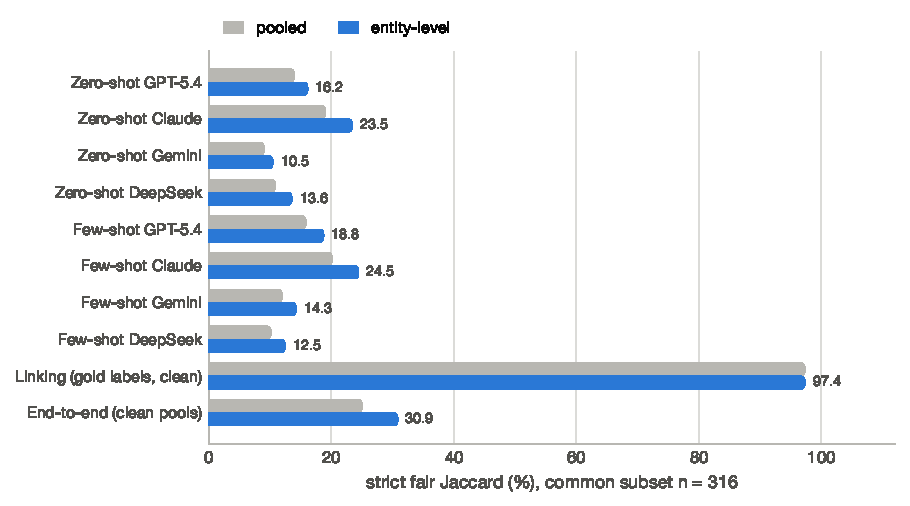
\includegraphics[width=0.88\textwidth]{figures/fig_main_comparison.pdf}
  \caption{Frozen models with and without the pipeline.}
  \label{fig:main}
  \tabnote{Strict fair set and common entity-defined subset.
The gold-label condition supplies the benchmark's query structure and is
used to isolate error sources; it is not presented as a performance
claim.}
\end{figure}

\subsection{Attributing the Error: Linking versus
Structure}

\label{sec:res-attribution}

For each question, the pipeline records whether it generated a query, whether all labels
were linked and whether the query executed.
\Cref{fig:funnel} shows these outcomes for the end-to-end
condition.

\begin{figure}[htbp]
  \centering
  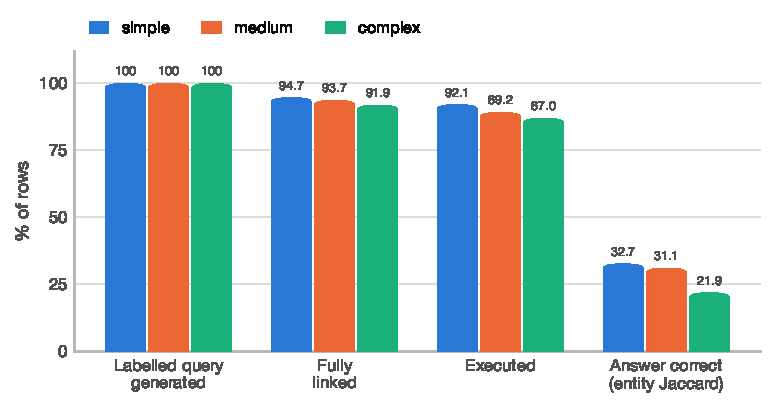
\includegraphics[width=0.88\textwidth]{figures/fig_stage_funnel.pdf}
  \caption{Stage-wise outcomes of the end-to-end pipeline, by query complexity.}
  \label{fig:funnel}
  \tabnote{Share of questions that pass each stage: labelled-query
generation, full linking, execution, and the final entity-level score.}
\end{figure}

Generation succeeds for 100\,\% of questions at every complexity level.
About 7\,\% of rows then lose a label during linking, and another 5\,\% fail to execute.
Final entity-level accuracy, over the 363 strict-set questions on which it is defined for this run, is 27.5\,\% and falls with complexity, from 32.7\,\% for simple questions to 21.9\,\% for complex ones.
On the common subset of 316 questions used to compare systems, the same run scores 30.9\,\% (\cref{tab:main}).

Most of the performance is lost at the final stage, but that alone does not isolate the cause.
Comparing the two conditions does.
On the common subset, given the benchmark's concepts and query structure, the pipeline reaches 97.4\,\%.
When it has to generate the query itself, it drops to 30.9\,\%, a difference of 66.5 points.
The gap therefore measures query generation, while disambiguation is measured directly in the linking comparison below.
The gap does not depend on the subset: on the full strict set of 400 questions, where a question without a scored query counts as zero, the two conditions reach 94.9 and 22.4 pooled Jaccard (\cref{tab:app-master}).

The gold-label condition is nearly tautological, because only the identifiers remain to be filled in, so it is not a performance result in itself.
Its value lies in the comparison between the two conditions.
The gap might suggest that structure explains all 66.5 points, but ``structure'' would then absorb every remaining source of error.
\Cref{fig:gap} breaks the gap down using the annotated failure sample.
Structural failures, that is the structure category together with the single triple flip (15 of 30 cases), make up 50.0\,\% of failing rows (95\,\% Wilson interval 33.2--66.8\,\%).
Applied to the 66.5-point gap, this share corresponds to 33.2 points.
Projection mismatches and residual identifier errors each account for about one fifth.
Structure is therefore the largest single component, especially for complex questions, while the rest of the gap comes from these other errors.
These figures are proportions of failing rows, not shares of the accuracy deficit, and they come from a 30-case sample (re-annotation agreement $\kappa$=0.62; agreement with an independent second annotator $\kappa$=0.595).

A second comparison changes only the candidate pools.
Building the pools with the rate-limited retrieval described in the method chapter raised gold-label accuracy by about 26 points, but end-to-end accuracy by only 2.6.
Better disambiguation thus helps a great deal when it is the only remaining task, and very little when the model also has to choose the concepts and build the structure.
This fits query generation being the main bottleneck.
The conclusion also does not rest on the annotated sample alone: the failure analysis examines construct use across all 567 reference queries and every generated run.

\begin{figure}[htbp]
  \centering
  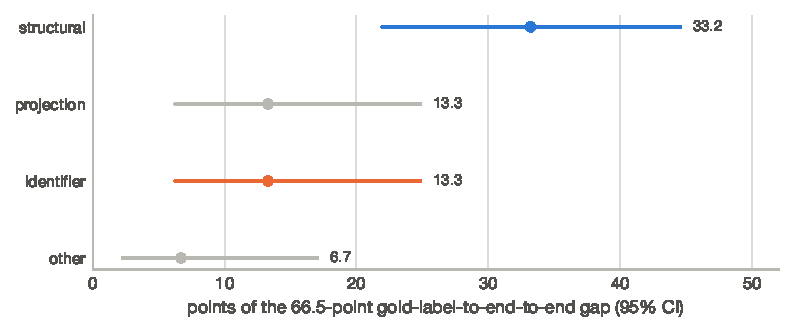
\includegraphics[width=0.88\textwidth]{figures/fig_gap_decomposition.pdf}
  \caption{What the 66.5-point gap is made of.}
  \label{fig:gap}
  \tabnote{Proportional attribution based on the 30-case taxonomy,
with Wilson intervals. The values are shares of failing rows, not of
the accuracy deficit.}
\end{figure}

\section{Linking Performance and Backbone
Dependence}

\subsection{Comparison of Linking
Paradigms}

\label{sec:res-linkers}

In the linking stage, every label in a query has to be mapped to the correct Wikidata identifier.
For each linker, precision, recall and F1 are computed at mention level against the ground truth derived from the benchmark: a prediction counts as correct only if it matches the reference identifier exactly, and a mention left unresolved counts against recall.

\begin{table}[htbp]
  \centering
  \caption{Entity and property linking across four paradigms, both splits.}
  \label{tab:linkers}
  \small
  \setlength{\tabcolsep}{3pt}
  \begin{tabular}{lllrrrr}
    \toprule
    Split & Linker & Backbone & Mentions & P (\%) & R (\%) & F1 (\%) \\
    \midrule
    working & Reasoning over candidates & Claude Opus 4.8 & entity & 97.8 & 97.6 & 97.7 \\
    working & Reasoning over candidates & Claude Opus 4.8 & property & 98.7 & 98.4 & 98.5 \\
    working & Reasoning over candidates & Qwen2.5-14B-Instruct & entity & 95.0 & 94.8 & 94.9 \\
    working & Reasoning over candidates & Qwen2.5-14B-Instruct & property & 98.0 & 97.7 & 97.9 \\
    working & Reasoning over candidates & Qwen2.5-7B-Instruct & entity & 95.8 & 95.7 & 95.8 \\
    working & GLiNKER gliner-linker-large-v1.0 & - & entity & 74.6 & 71.0 & 72.8 \\
    working & ELQ elq\_wiki\_large & - & entity & 67.1 & 18.0 & 28.4 \\
    working & ReFinED questions\_model & - & entity & 79.7 & 15.9 & 26.6 \\
    working & First search result & - & entity & 93.6 & 93.5 & 93.5 \\
    official & Reasoning over candidates & Qwen2.5-14B-Instruct & entity & 93.1 & 92.6 & 92.9 \\
    official & Reasoning over candidates & Qwen2.5-14B-Instruct & property & 97.8 & 97.0 & 97.4 \\
    official & GLiNKER gliner-linker-large-v1.0 & - & entity & 72.5 & 69.7 & 71.0 \\
    official & ELQ elq\_wiki\_large & - & entity & 71.7 & 22.1 & 33.8 \\
    official & ReFinED questions\_model & - & entity & 77.2 & 16.4 & 27.1 \\
    official & First search result & - & entity & 90.5 & 90.0 & 90.2 \\
    \bottomrule
  \end{tabular}
  \tabnote{Identical rows, identical ground truth and identical candidate pools within each split. P/R/F1 are mention-level; a prediction counts as correct only on exact identifier match. ELQ and ReFinED detect their own mentions, so their set-based figures are reported in the text instead. GLiNKER chooses among the same seven candidates per label as the reasoning linker. \emph{First search result} takes the first Wikidata search hit among those candidates, without any model, as a reference. Per-complexity F1 is plotted in Figure~\ref{fig:linker-cx} rather than repeated here.}
\end{table}


Four linking implementations were evaluated on the same rows, with the same ground truth, the same candidate pools where applicable, and the same scoring code.
The comparison is not fully symmetric: the reasoning-based linkers and GLiNKER choose from labels and curated candidates, whereas ELQ and ReFinED have to detect mentions in the question text themselves (see the limitations).
The paragraphs below assess how much of the ordering this difference explains.
\Cref{fig:linkers} shows entity-linking F1 on both splits, and~\cref{tab:linkers} gives the results.

\begin{figure}[htbp]
  \centering
  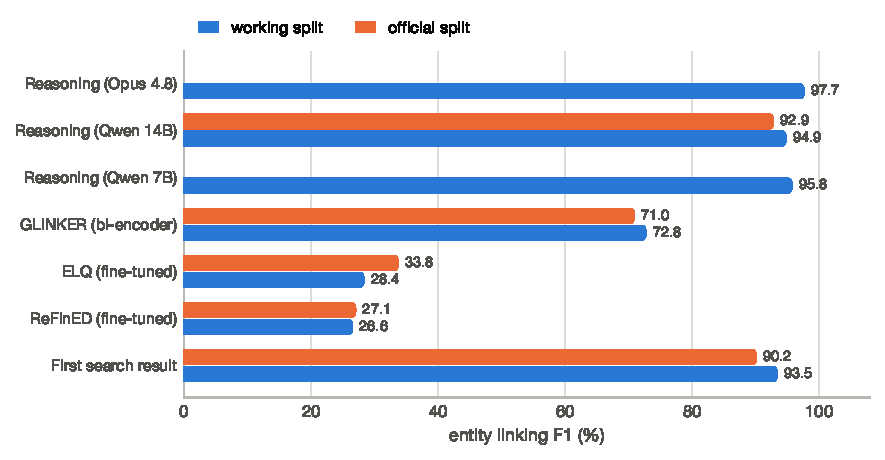
\includegraphics[width=0.88\textwidth]{figures/fig_linker_comparison.pdf}
  \caption{Entity linking F1 across four paradigms and two splits.}
  \label{fig:linkers}
  \tabnote{Within each split, all systems use identical rows,
ground truth and candidate pools. The first search result is a
reference without any model. On the official split, the reasoning
linker was run with the Qwen2.5-14B backbone only, which is available on
the group's GPU server; Claude Opus 4.8 (paid API) and Qwen2.5-7B were
evaluated on the working split.}
\end{figure}

With a frontier backbone, reasoning over retrieved candidates reaches 97.7 entity F1 and 98.5 property F1, and it resolves every identifier correctly in 89.9\,\% of queries.
The specialised linkers score lower: 72.8 (GLiNKER, choosing among the same candidates), 28.4 (ELQ) and 26.6 (ReFinED).
\Cref{fig:linker-ci} reports bootstrap confidence intervals for these scores, resampling the 1,086 entity mentions with replacement and applying the same resample to every linker in each draw.
The paired difference between the frontier reasoning linker and GLiNKER is 24.9 points $[22.3, 27.7]$, about five times the width of its own interval.
A reference point without any model shows where this accuracy comes from: taking the first Wikidata search result for each label reaches 93.5 on the working split and 90.2 on the official split.
Reasoning over the candidates adds 4.1 points $[2.7, 5.6]$ to it with the frontier backbone, 2.2 with Qwen2.5-7B and 1.4 with Qwen2.5-14B, the last within noise.
So most of the linking accuracy comes from labels that Wikidata's search can find, and the reasoning step resolves the remaining ambiguous cases, while GLiNKER's choice falls below the search order itself.
The intervals of the three reasoning backbones overlap, so they are not ranked against each other.
This similarity is the main finding of the backbone comparison below.

\paragraph{The Shape of the Deficit}

The specialised linkers' errors follow a clear pattern.
\Cref{fig:linker-pr} shows that ELQ and ReFinED, although developed independently, years apart and with different architectures, share a similar precision–recall profile (precision 67--80\,\%, recall 16--22\,\%): when they predict, they are usually right, but they do not predict often enough.
\Cref{fig:linker-cx} breaks F1 down by complexity: the two fine-tuned linkers are the only systems whose F1 falls as complexity rises (ReFinED 53.7$\to$35.6$\to$20.3; ELQ 34.1$\to$37.2$\to$23.3), while the linkers that choose among candidates hold steady or improve (frontier 92.9$\to$98.1$\to$97.7; GLiNKER 61.8$\to$70.7$\to$74.1).
This fits the mention-detection mismatch discussed earlier.
The set-based metric, which removes the mention-alignment penalty, lifts ELQ to 33.8 and ReFinED to 33.4 and so explains part, but not most, of the deficit.
ELQ's entity library, derived from Wikipedia in 2019, contains 72.4\,\% of the reference entities in the official split and 68.6\,\% in the working split.
So missing entities explain only a small part of a recall of 18--22\,\%, and mention detection most of it.

GLiNKER was evaluated outside the setting it was designed for, and ELQ and ReFinED solve a different sub-task because they detect their own mentions.
Neither issue, alone or combined, explains the ordering.
Given the same seven candidates as the reasoning linker, GLiNKER reaches 72.8 with candidate descriptions and 41.8 with labels alone, so the descriptions carry most of its gain.
The ordering holds on both splits: on the official split, GLiNKER reaches 71.0 against 92.9 for the reasoning linker with Qwen2.5-14B.

\paragraph{Replication on LC-QuAD 2.0}

Both splits come from the same dataset, so they cannot show whether the result carries over to other benchmarks.
Repeating the experiment on LC-QuAD 2.0 (gold-label condition; backbone, candidate depth, prompt and scoring held constant; 150 questions, 203 entity and 250 property mentions) gives 90.6\,\% entity accuracy $[85.8, 93.9]$ and 96.4\,\% property accuracy $[93.3, 98.1]$, with 96.7\,\% of queries fully linked.
The pattern found on Instruct-to-SPARQL reappears on a benchmark with different authors, templates and aims.

Entity accuracy is 4.3 points below the 94.9\,\% the same backbone reaches on Instruct-to-SPARQL, which lies outside the reported interval and cannot be explained by sampling noise alone (LC-QuAD 2.0 may contain more long-tail entities).
Unlike the labels in Instruct-to-SPARQL's annotated variant, its mention labels are the current Wikidata labels of the gold identifiers and are therefore findable by construction.
The reported value is an upper bound for this benchmark, and the comparison across benchmarks matters more than the absolute level.
This experiment replicates the linking measurement only.
The structural gap is measured on Instruct-to-SPARQL.
Separately, six of the 357 gold identifiers in the sample (1.7\,\%) no longer resolve against Wikidata, because they have been deleted or merged since the benchmark was published in 2019.

\subsection{Backbone Dependence by
Stage}

\label{sec:res-lcquad}

\label{sec:res-backbone}

The reasoning-based linker was evaluated again with two open-weight backbones, with the prompt, candidate pools, ground truth and evaluation procedure unchanged.
\Cref{fig:backbone} shows the results, which differ sharply between the disambiguation and label-generation stages.

\begin{figure}[htbp]
  \centering
  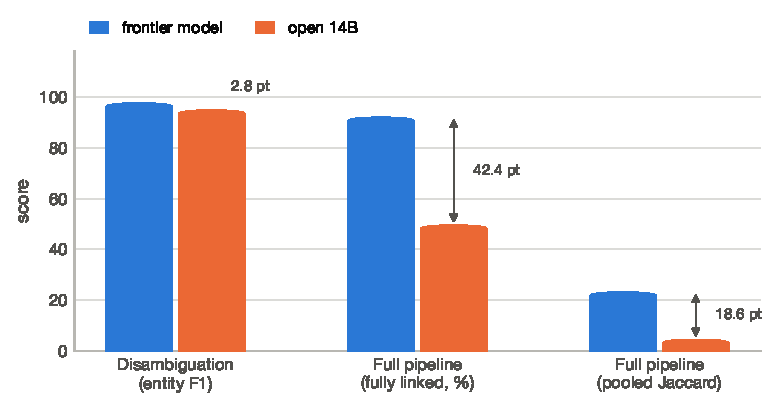
\includegraphics[width=0.88\textwidth]{figures/fig_backbone.pdf}
  \caption{Disambiguation and label-generation results by backbone.}
  \label{fig:backbone}
  \tabnote{Frontier model against the open 14B model: entity F1 at the
disambiguation stage (working split), and the fully linked rate and pooled
Jaccard of the official-split pipeline when the respective model generates
the labelled query.}
\end{figure}

At the disambiguation stage, the backbone makes little difference.
The frontier model reaches 97.7 entity F1, the 14-billion-parameter open model 94.9, and the 7-billion-parameter open model 95.8, with overlapping confidence intervals.

During label generation, the backbone matters more.
On the official split, using the open model for both stages drops the linked rate from 92.1\,\% to 49.7\,\%, and pooled accuracy from 23.4 to 4.8.

\Cref{fig:labelfail} shows why.
Asked to produce Wikidata entity and property labels on its own, the open model writes 270 of 1,645 distinct labels (16.4\,\%) that Wikidata's search index cannot find.
The frontier model writes 23 of 687 such labels (3.3\,\%) on the same questions.
The open model's failure rate is 4.9 times higher.

About half of the open model's unfindable labels are near-misses of existing property names, such as ``crew member(s)'' and ``is named after''.
Another 29\,\% are camelCase RDF-style identifiers, such as locatedInTheAdministrativeTerritory.
A further 3\,\% use snake\_case, and 2\,\% are bare property identifiers where a label was expected.
The frontier model produces none of these last three kinds.
The open model also generates 2.4 times as many distinct labels for the same questions, a sign of both lower consistency and lower accuracy.

\begin{figure}[htbp]
  \centering
  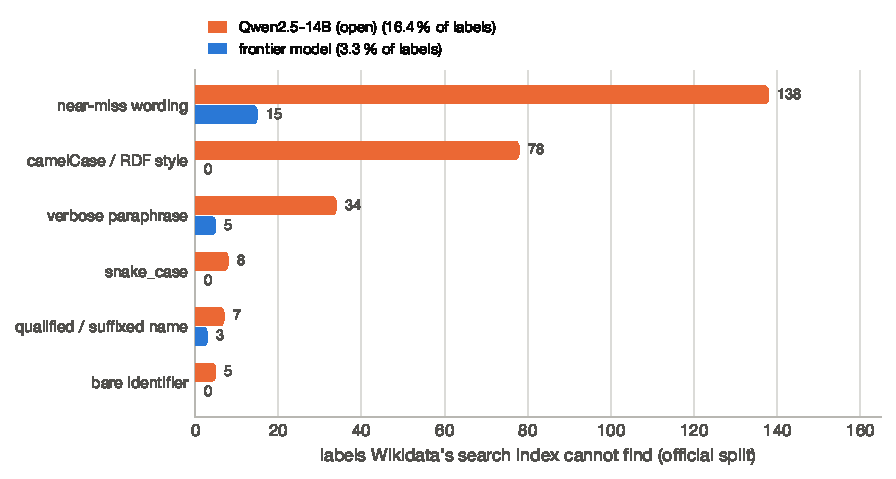
\includegraphics[width=0.88\textwidth]{figures/fig_label_failures.pdf}
  \caption{Unfindable labels by failure type and backbone.}
  \label{fig:labelfail}
  \tabnote{The figure includes labels that the Wikidata search index
cannot find. The official split is used, and labels are deduplicated
separately for both backbones. camelCase, snake\_case and bare
identifiers occur only for the open model and account for 34\,\% of its
unfindable labels.}
\end{figure}

One possible explanation is that the open model mainly has a formatting problem that a deterministic fix could solve.
This was tested with a normalisation procedure that splits camelCase, removes underscores, drops a leading ``is'' or ``has'', removes trailing parentheticals and singularises terms.
All 270 labels were normalised and searched again.

The procedure repaired 43 labels (15.9\,\%), lowering the failure rate from 16.4\,\% to 13.8\,\%.
Splitting camelCase recovered 36\,\% of the labels in that category, but such mechanical cases were only a minority of the failures.
The largest category could not be repaired, because terms such as ``significant achievement'' are alternative names for existing Wikidata properties.

The difference between the backbones at the generation stage is mainly a matter of knowing Wikidata's vocabulary.
Neither surface formatting nor reasoning ability explains it.
The next chapter discusses the practical implications.

\paragraph{Replication with Claude Opus 5}

All results so far use one frontier generator, so the diagnosis might reflect that particular model.
The baseline condition was therefore repeated with Claude Opus 5.
Nothing else changed: the system prompt, the absence of extended thinking, the disambiguation backbone and the scoring procedure stayed the same.

Accuracy rose from 27.03 to 32.66 entity-level Jaccard over 354 paired rows.
The construct counts show, however, that the improvement was uneven.

Compliance with subclass closure rose from 19.5\,\% to 43.6\,\%, and compliance with property paths from 13.4\,\% to 36.6\,\%.
Statement-node use increased from 18.5\,\% to 22.3\,\%, and qualifier use from 22.4\,\% to 28.2\,\%.
Value-node use did not improve at all: of the 35 reference queries that need a value node, both models use one in only two (5.7\,\%), and Opus 5 uses value nodes three times in total.

The newer model is much better at constructs that are mainly a matter of SPARQL syntax, and improves far less on constructs that require understanding how Wikidata represents information.
This mirrors the distinction drawn in the failure analysis below, between general-purpose SPARQL constructs, which models already use fairly often, and Wikidata-specific reification and hierarchy idioms, which remain difficult.

Opus 5 fully links 92.6\,\% of the 567 questions, against 95.2\,\% for Opus 4.8.
It produces six empty generations, where the earlier model produces none, and leaves 34 of 778 labels unresolved, against 25 of 852.
The candidate pool was pre-seeded and no rate limiting occurred, so these differences come from the backbone itself.
The newer model writes somewhat more labels that Wikidata's search index cannot find, which means its accuracy gain comes despite a slightly lower linking rate.

\section{Structural Failure
Analysis}

\label{sec:error-analysis}

The main failure pattern is characterised with evidence of increasing sample size: an annotated failure sample, construct counts across the corpus, and features of the reference queries.
The smallest is the easiest to interpret, and the largest gives the strongest evidence at corpus level.

\paragraph{Error Taxonomy}

\begin{table}[htbp]
  \centering
  \caption{Error taxonomy of a stratified sample of 30 failing questions.}
  \label{tab:errors}
  \small
  \resizebox{\ifdim\width>\textwidth\textwidth\else\width\fi}{!}{%
  \begin{tabular}{lrr}
    \toprule
    Category & n & Share (\%) \\
    \midrule
    structure & 14 & 46.7 \\
    near miss (projection) & 6 & 20.0 \\
    wrong property & 3 & 10.0 \\
    execution error & 2 & 6.7 \\
    unresolved label & 2 & 6.7 \\
    triple flip & 1 & 3.3 \\
    reference noise & 1 & 3.3 \\
    wrong entity & 1 & 3.3 \\
    \bottomrule
  \end{tabular}}
  \tabnote{Complexity-stratified random sample (seed 42) drawn from the reported clean-pool run and categorised by dominant error type. Each case was categorised by the author; an independent second annotator agreed on 21 of 30 cases. Proportions are indicative rather than population estimates.}
\end{table}


A complexity-stratified random sample of thirty failing questions was drawn from the reported end-to-end run, and each was classified by its dominant error type.
\Cref{fig:errors} and~\cref{tab:errors} show the distribution: structure accounts for 46.7\,\%, near misses for 20.0\,\%, wrong properties for 10.0\,\%, execution and unresolved errors for 6.7\,\% each, and triple flips, reference noise and wrong entities for 3.3\,\% each.
The gap attribution above groups the one triple flip with structure, because the query has the right properties but the wrong shape, which gives the structural group 15 of the 30 cases.

Structural errors are the largest category at every complexity level and are common among complex questions. Ten of the fifteen complex failures are structural.
Identifier-related errors still occur, though; three of the fifteen complex failures (20\,\%) come down to identifier selection.

The author categorised the cases in a single annotation pass, so the proportions describe recurring failure modes and should not be read as population-level frequencies.

\paragraph{Annotation Reliability}

To check the reliability of the categorisation, ten of the thirty cases were selected with an independent seed, anonymised and shuffled, and then re-annotated by the same person without access to the first classification.
Raw agreement was 7 of 10, and Cohen's $\kappa$ was 0.62, which is conventionally regarded as substantial agreement.

Two of the three disagreements concerned the boundary between structural and wrong-property errors, which is exactly the distinction the attribution analysis depends on.
Under the second annotation, the structural group fell from 15 to 14 of the 30 cases (50.0\,\% to 46.7\,\%), and the identifier-related share rose from 20.0\,\% to 26.7\,\%.
Structure stayed the largest single category, but by a smaller margin.

The second annotation also distinguished between an incorrect constraint, a missing constraint and missing aggregation.
The current taxonomy groups these cases under ``structure'', so the category is fairly broad.

\paragraph{A Second, Independent
Annotator}

Consistency within one annotator does not show that others read the categories the same way.
A second annotator, an undergraduate computer science student not involved in the project, classified all thirty cases independently, using only the written category guide, which is provided in the accompanying repository.

Raw agreement was 21 of 30, and Cohen's $\kappa$ was 0.595, slightly below the intra-annotator value.
The two annotators gave similar estimates for the category: the structure category accounted for 46.7\,\% of cases according to the author and 43.3\,\% according to the second annotator.
Only two of the nine disagreements concerned the boundary between structure and wrong-property errors.

The attribution therefore holds across two annotators.
Four of the nine disagreements, however, involved the quality of the reference query.
The second annotator pointed out specific issues: a missing country constraint, a missing class restriction, a grouped count where the question asked for items, and a flag that was computed but never used as a filter.
These judgements raise the estimated reference-noise rate in the sample from 3.3\,\% to 16.7\,\%.
Thirty rows cannot establish the true rate, so it is estimated on the full split below.

\paragraph{Bounding the Rate of Reference
Noise}

The full split was screened with five rules derived from the disputed cases (e.g.\ a superlative question whose reference query has no ordering or limit, or a nationality question whose reference has no country property), which flagged 61 of 400 strict-set queries (15.2\,\%).
A flag rate is not a noise rate, so a stratified sample of 40 flagged and 40 unflagged queries was adjudicated one by one (24 were dropped as unexecutable on the current snapshot, leaving 26 flagged and 30 unflagged).
Half of the flagged queries were judged faulty, against 6.7\,\% of the unflagged ones, which gives an initial estimate of 13.3\,\%.

A second independent judge, a doctoral student in computer science who was blind to the author's decisions and to the sampling strata, reviewed the same 56 rows.
Agreement was 73.2\,\% ($\kappa$=0.426).
The second judge's estimate was 32.0\,\%, against 13.3\,\% for the author.
The disagreement was systematic: 12 of the 15 cases went the same way, and they came from detection rather than from different standards of correctness. The author's first pass relied on the executed output, while the second judge also read the query text and caught issues such as a commented-out deduplication filter or an unchecked \texttt{OPTIONAL} block.

The two judges then reconciled the fifteen disagreements together against the query text and resolved ten in the second judge's favour.
The reconciled estimate is \textbf{24.6\,\% of the strict fair set, with an interval of $[12.9, 42.0]$}.
This counts the five cases that remained unresolved (genuine ambiguity about the intent of a loosely written question, not a checkable fact) as sound; counting them as faulty gives 32.0\,\%, the same as the second judge's independent estimate.
Reconciliation also showed that the screen's weakness is recall, not precision: its accuracy on the flagged group was unchanged (13/26 both before and after), while the fault rate in the unflagged group rose from 6.7\,\% to 20.0\,\%.

Roughly one quarter of the reference queries may therefore be unsound.
Some failures attributed to query structure may then come from the benchmark, and a system may be penalised for correctly answering a question that the benchmark encodes incorrectly.
The reported accuracy figures are not corrected for reference noise, for the comparability reasons discussed in the limitations.

\paragraph{Mechanism}

The structural failures follow a clear pattern: the model writes syntactically valid SPARQL but uses the direct-claim shortcut \texttt{wdt:} where the reference needs a more complex construct, such as transitive subclass closure, statement qualifiers, normalised value nodes, explicit aggregation, alternation, the lexeme model, or sitelink/badge access.
General-purpose SPARQL is handled well; the deficit is confined to Wikidata's reification and hierarchy idioms.
Averaging a height property directly instead of through its normalised value node, for example, silently mixes units and yields an arithmetically wrong result that the syntax alone does not reveal.
Near misses caused by projection mismatches, where the query returns a relation's object instead of its subject, were checked separately on ten additional zero-scoring rows.
All ten were indeed incorrect, so the reported accuracy needs no adjustment.
One further case in the sample was a reference query that did not answer its own question, an early sign of the reference-noise problem quantified above (24.6\,\% $[12.9, 42.0]$).

\paragraph{Corroboration across the
Corpus}

Because the sample is small, the same mechanism was tested at corpus scale across all 567 reference queries and every generated run (\Cref{fig:constructs}).

\begin{figure}[htbp]
  \centering
  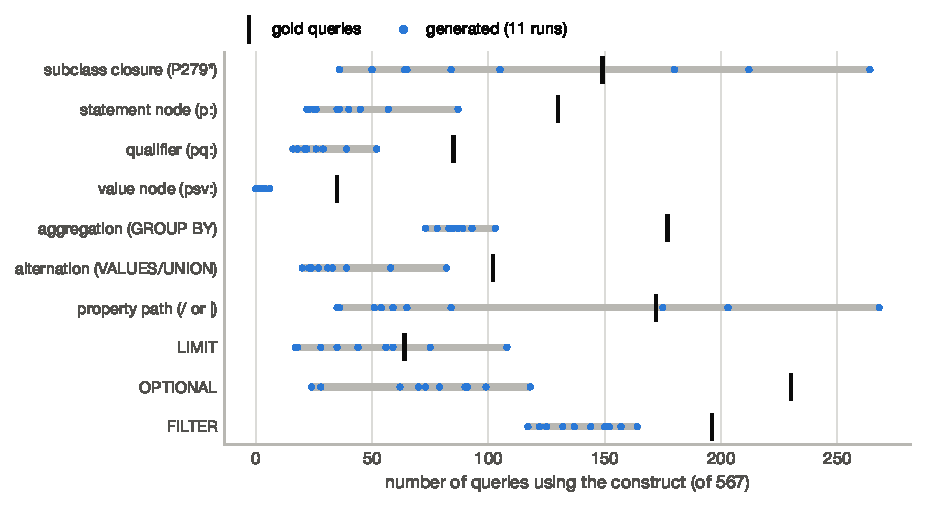
\includegraphics[width=0.88\textwidth]{figures/fig_constructs.pdf}
  \caption{Use of Wikidata's constructs: gold queries against all generated runs.}
  \label{fig:constructs}
  \tabnote{Each row shows the minimum and maximum count across the
eleven generated runs, while the rule indicates the count in the
reference queries.}
\end{figure}

Every system underuses Wikidata-specific constructs: of the 130 reference queries that use statement nodes, generated systems use them in 22--87; of 85 with qualifiers, in 16--52; and of 35 with normalised value nodes, in 0--4 (the strongest baseline never uses them).
General-purpose constructs (\texttt{FILTER}, \texttt{GROUP BY}, \texttt{OPTIONAL}) appear at rates close to the reference, so the deficit is specific to reification and hierarchy idioms, and it shows up across all four model families and both prompting regimes.

Usage counts alone cannot tell a system that never uses a construct from one that uses it in the wrong places, so~\Cref{fig:agreement} reports construct-agreement F1 instead.
Agreement is low and does not follow usage frequency: zero-shot GPT-5.4 uses subclass closure 212 times against 149 in the reference, yet agrees on only 54.8\,\% of questions, applying it where it is not needed and leaving it out where it is.
Only general-purpose constructs reach the 55--60 range.
So the models misplace these constructs as well as underusing them.

\begin{figure}[htbp]
  \centering
  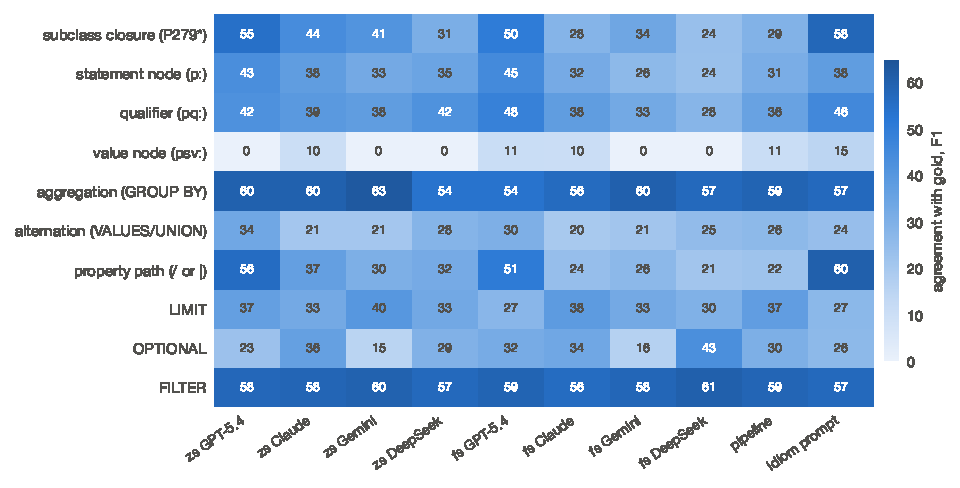
\includegraphics[width=0.88\textwidth]{figures/fig_construct_agreement.pdf}
  \caption{Agreement with gold on construct use, by system.}
  \label{fig:agreement}
  \tabnote{The figure reports per-question F1 for using a construct
exactly where it appears in the reference query. Usage counts alone
cannot distinguish missing use from excessive use, and agreement
measures both.}
\end{figure}

Finally, features of the reference query correlate with achieved accuracy in the expected direction (\cref{fig:predictors}): aggregation goes with 12.6 points lower accuracy, value nodes with 10.1, alternation with 9.6, transitive closure with 8.6 and statement nodes with 8.2, while \texttt{OPTIONAL} is the only feature linked to higher accuracy ($+10.9$).
These are weak differences in group means ($|\rho|\leq 0.15$), not predictive relationships.
They are reported because their ordering agrees with the taxonomy and the construct counts, so three independent measurements point in the same direction.
If this diagnosis is correct, telling the model explicitly about these constructs should help.

\section{Prompt Interventions and
Recovery}

\label{sec:res-noise}

\subsection{Prompt Interventions}

\label{sec:res-prompts}

\begin{table}[htbp]
  \centering
  \caption{Prompt interventions against the baseline arm: paired tests.}
  \label{tab:significance}
  \small
  \resizebox{\ifdim\width>\textwidth\textwidth\else\width\fi}{!}{%
  \begin{tabular}{lrrrrrr}
    \toprule
    Comparison & n & Mean difference (pp) & CI low & CI high & Permutation $p$ & Wilcoxon $p$ \\
    \midrule
    idiom guidance & 354 & 3.88 & 1.18 & 6.66 & 0.0054 & 0.0581 \\
    schema evidence, verbose & 336 & -14.65 & -18.94 & -10.38 & <0.001 & <0.001 \\
    schema evidence, targeted & 339 & -12.66 & -17.35 & -8.1 & <0.001 & <0.001 \\
    construct profile & 355 & 3.0 & 0.2 & 5.75 & 0.0342 & 0.0693 \\
    constrained vocabulary & 356 & 18.99 & 15.03 & 23.11 & <0.001 & <0.001 \\
    both oracles & 353 & 23.01 & 18.69 & 27.39 & <0.001 & <0.001 \\
    \bottomrule
  \end{tabular}}
  \tabnote{Paired over questions scored in both arms. Confidence intervals are bootstrap percentile intervals; the permutation test is two-sided. Only the generation prompt differs between arms.}
\end{table}


Seven generation conditions were compared, differing only in their system prompts.
\Cref{fig:arms} shows accuracy by intervention and the paired difference against the baseline, and~\cref{tab:significance} reports the statistical tests.
With a Holm correction for the six comparisons, every permutation result stays below 0.05.
The Wilcoxon signed-rank test, which uses the ranks rather than the sizes of the paired changes, is above 0.05 for idiom guidance (0.058) and the construct profile (0.069).

Idiom guidance gives a modest improvement.
Averaged over the questions each arm scored, entity-level accuracy rises from 26.8 to 30.2.
Over the 354 questions scored in both arms, the paired difference is $+3.88$ points $[1.18, 6.66]$, with a permutation result of $p = 0.005$.
The gain grows with query complexity, in line with the error analysis, where structural failures dominate at high complexity.

The average gain hides variation between questions, however.
Seventy questions improve, while 68 get worse.
The intervention shifts the overall level and distribution of performance, but it does not improve individual questions systematically.

Schema evidence has the opposite effect.
Averaged over the questions each arm scored, the verbose version lowers accuracy to 13.0 and the targeted version to 14.5.
The paired differences are $-14.65$ and $-12.66$, both with $p < 0.001$.
This runs against the improvements reported in research on schema-aware grounding, including~\parencite{zhang2026saga}.
The loss is about four times as large as the gain from idiom guidance.
It does not follow that retrieval augmentation is harmful in general: systems that combine retrieved context with an explicit validation or correction layer, rather than unconstrained prompt text, report gains from the same broad strategy~\parencite{pan2025firesparql}.
The finding here concerns schema evidence presented as evidence, not as a constraint.

\begin{figure}[htbp]
  \centering
  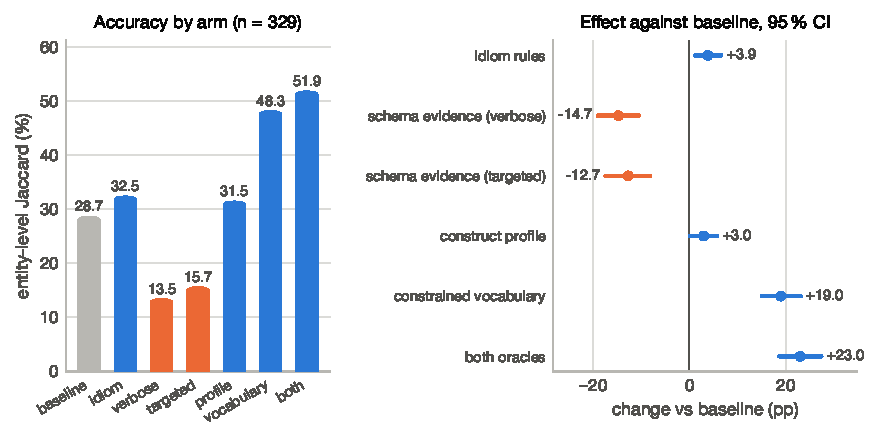
\includegraphics[width=0.88\textwidth]{figures/fig_prompt_arms.pdf}
  \caption{Prompt interventions: accuracy by arm and effect against the baseline.}
  \label{fig:arms}
  \tabnote{Only the generation prompt differs between conditions. The
generation model, candidate pools, disambiguation backbone and scoring
procedure remain constant. The left panel shows mean accuracy on the 329
rows scored in every arm. These levels are comparable across arms but
are slightly higher than the pairwise values in the text because the
latter use each comparison's own common rows. The right panel shows the
paired difference against the baseline with a 95\,\% bootstrap interval.}
\end{figure}

\paragraph{What the Interventions
Change}

\Cref{fig:idiom} shows how idiom guidance changes the generated queries: subclass closure rises from 50 to 264 (reference: 149), statement-node use from 25 to 45 (reference: 130), value-node use from 2 to 6 (reference: 35), and unrequested \texttt{LIMIT} clauses fall from 59 to 18.
Construct agreement improves most for the two constructs the prompt stresses most (subclass closure 29\,\%$\to$58\,\%, property paths 22\,\%$\to$60\,\%).
The prompt changes behaviour a lot, sometimes pushing simple syntactic constructs past the reference rate, but it does much less for constructs that require knowing how Wikidata represents information.
Value-node use barely moves, and aggregation does not change at all despite an explicit instruction to use it.

The construct counts suggest that over-application is the main way the grounding interventions fail: against reference counts of 149 subclass closures, 130 statement nodes and 85 qualifiers, the targeted schema arm produces 342, 256 and 142.
Shorter, conditional evidence increases over-application instead of reducing it.
The grounded arms also share only 38\,\% of their label vocabulary with the baseline, compared with 73\,\% for the idiom arm.
Schema evidence leads the model to rewrite its queries extensively, even though the schema cards were built from reference-linked mentions, a favourable setting in which the intervention fails.

\begin{figure}[htbp]
  \centering
  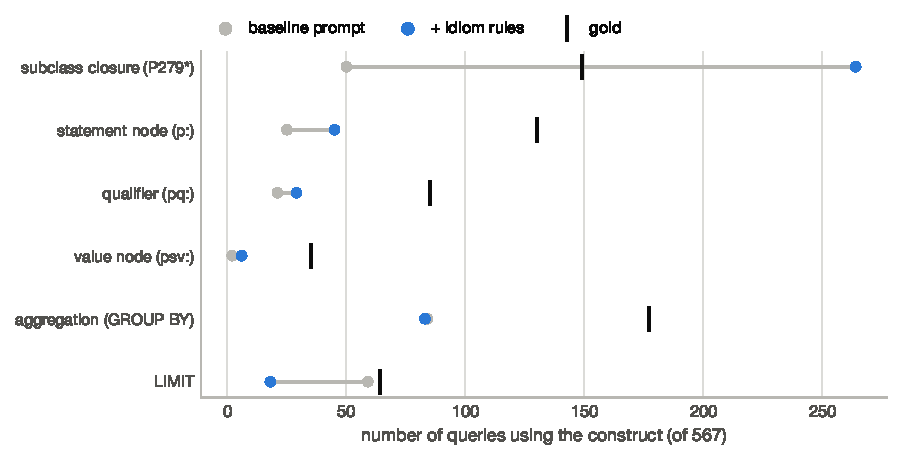
\includegraphics[width=0.88\textwidth]{figures/fig_idiom_behaviour.pdf}
  \caption{What the idiom prompt changes in the generated queries.}
  \label{fig:idiom}
  \tabnote{Number of the 567 generated queries that use each
construct under the baseline prompt and with the idiom rules. The
vertical mark gives the count in the reference queries.}
\end{figure}

\paragraph{Applying Guidance
Selectively}

If over-application is the problem, guidance could be given only when a query needs the relevant construct.
That requires two conditions, and the results fully support neither.
First, the need must be predictable from the question: a classifier that uses only the question text predicts construct use with an AUC of 0.62--0.82.
For subclass closure, its strongest features are topical terms (``libraries'', ``hospitals'', ``scientists''), because whether closure is needed depends on how Wikidata models the domain as well as on how the question is worded.
Second, guidance must do harm where it is not needed, and the results do not show this: idiom guidance helps most when the reference needs subclass closure ($+9.72$) or value nodes ($+7.97$), but it still raises accuracy by 2.0--4.3 points when no idiom is required.
On the 354 questions scored in both arms, an oracle gate that gives guidance only when a reification or hierarchy construct is present reaches 30.1, below the 31.2 of giving it unconditionally.
Selective application therefore does not beat always-on guidance, even with perfect knowledge of need, because over-application costs little.

\paragraph{Supplying the Knowledge
Directly}

If generic and selective guidance do not close the gap, the next question is what the model does when the missing knowledge is supplied directly.
Two interventions test two different kinds of information.

The construct-profile arm gives oracle information about which constructs the reference query uses, without revealing the query itself.
The model follows this information almost completely.
Subclass-closure compliance rises from 19.5\,\% to 100\,\%, and property-path compliance from 13.4\,\% to 95.3\,\%.
Compliance is lower for constructs that need more knowledge of how Wikidata stores facts, at 57.1\,\% and 61.2\,\%.

Despite this near-complete compliance, accuracy rises by only $+3.00$ points $[0.20, 5.75]$, no different from the gain from generic idiom guidance.
For the fourth research question, this means that the model can be told exactly which idiom is needed, and it will mostly use it, yet this adds little.
Knowing which construct is required is not the main bottleneck.

The constrained-vocabulary arm supplies a different kind of information.
It gives a closed list of the entities and properties that the reference query uses and forbids the model to use any identifier outside that list.
Accuracy rises by $+18.99$ points $[15.03, 23.11]$, with $p < 0.001$.
Here 141 questions improve and 41 get worse, which makes it the only intervention whose effect is consistently positive.

This is not a standalone performance claim: like the gold-label condition, the intervention receives part of the answer in advance, so its absolute performance is partly definitional.
The result is meaningful as a comparison, because the enumerative schema cards were built from the same reference-linked mentions.

The two arms receive information about the same entities and differ only in how it is presented.
Given as available evidence, it lowers accuracy by 14.65 points.
Given as a closed vocabulary that the model must use, it raises accuracy by 18.99 points.
The resulting difference of 34 points, with non-overlapping intervals, motivates the design principle discussed in the next chapter. Prompt-level intervention can still help, but more advice alone does not.

\paragraph{Which Knowledge Matters: A
Two-by-Two}

The two single-factor interventions supply different information and produce very different gains.
They correspond to the two generation decisions defined in the method chapter: the permitted vocabulary settles concept selection, and the construct profile names the idioms that structural composition needs.
A fourth arm, supplying both, completes a factorial design (percentile intervals from 10,000 bootstrap resamples) and shows that the effects are additive: construct information adds $+3.76$ points $[0.96, 6.58]$ even with the concepts fixed, and concept information adds $+19.72$ points $[15.30, 24.03]$ even when the required constructs are specified.
The jointly predicted result (21.99) matches the observed 23.01, and the one-point interaction lies within the intervals.
Concept selection thus accounts for the larger part of the error that these two oracles remove, and naming the idioms adds a smaller, independent part.
Neither oracle composes the query: with both supplied, entity-level accuracy reaches 50.4 on the 353 paired questions, whereas the gold-label condition, which supplies the composed query, reaches 97.4.
The model can recognise and use a named construct but still struggles to compose the correct query around the right concepts.

\paragraph{Type-Constraint Filtering}

The constrained-vocabulary arm restricts the generator through instructions, which it may ignore.
\citet{zhang2026saga} instead remove type-incompatible candidates mechanically before generation.
Filtering cannot be undone, so a removed candidate cannot be recovered by later reasoning.
The first thing to check is whether filtering keeps the correct property.
The test covers every property mention with at least two candidates including the reference property (1,132 mentions, 4.39 candidates on average).
A candidate is removed when it declares a Wikidata type constraint (P2302, constraint type Q21503250) and none of its permitted classes covers a subject type present in the question.
Subject types are taken from the row's reference entities via P31/P279 closure.
Of 1,062 candidate properties, 704 declare a type constraint.
Only 80 mark it as mandatory, while 616 have a type constraint without any status, so a violation is reported but not prohibited (a property can carry several such constraints).
Applying every declared constraint affects 79.8\,\% of mentions and shrinks the average pool from 4.39 to 3.02, but the reference property survives only 92.5\,\% of these operations.
Restricting the filter to mandatory constraints raises survival to 99.1\,\% but removes only about half a candidate per mention and resolves just three of the 1,132.

The two filters trade off differently: the stronger one removes the correct answer in roughly one of thirteen affected mentions, while the safer one removes almost nothing.
Even the safer estimate is generous.
The type universe combines all entity types in a row, subject types come from reference entities and not from a signal available at deployment, and forty-one mentions have no reference entity and would require abstention.

The principle of constraining rather than enumerating still holds, but implementing it mechanically is not straightforward.
Constraining the generator works when the constraint is correct.
A mechanical filter, however, is only as good as the quality and completeness of Wikidata's constraint declarations, and most of these are not marked as binding.

\subsection{Recovering Failures without Gold
Supervision}

\label{sec:res-filter}

\label{sec:res-cascade}

\begin{table}[htbp]
  \centering
  \caption{Selection strategies over diverse generations, entity-level Jaccard.}
  \label{tab:cascade}
  \small
  \resizebox{\ifdim\width>\textwidth\textwidth\else\width\fi}{!}{%
  \begin{tabular}{llrrr}
    \toprule
    Candidate pool & Selection & n & Entity-level Jaccard & Exact match (\%) \\
    \midrule
    one generator, three prompts & baseline arm & 349 & 26.3 & 8.3 \\
     & idiom arm & 349 & 30.2 & 11.5 \\
     & end-to-end run & 349 & 27.1 & 8.6 \\
     & cascade & 349 & 33.5 & 12.3 \\
     & centroid & 349 & 30.6 & 10.3 \\
     & centroid with fallback & 349 & 30.3 & 10.3 \\
     & oracle & 349 & 35.4 & 14.0 \\
    \midrule
    four zero-shot models & zero-shot Claude & 330 & 22.5 & 8.2 \\
     & zero-shot GPT-5.4 & 330 & 14.9 & 5.2 \\
     & zero-shot Gemini & 330 & 9.8 & 2.7 \\
     & zero-shot DeepSeek & 330 & 12.3 & 3.9 \\
     & cascade & 330 & 23.7 & 8.2 \\
     & centroid & 330 & 24.5 & 8.5 \\
     & centroid with fallback & 330 & 24.2 & 8.5 \\
     & oracle & 330 & 28.0 & 10.9 \\
    \midrule
    all eight runs & idiom arm & 327 & 32.2 & 12.2 \\
     & end-to-end run & 327 & 29.0 & 9.2 \\
     & baseline arm & 327 & 28.1 & 8.9 \\
     & few-shot Claude & 327 & 23.4 & 7.3 \\
     & zero-shot Claude & 327 & 22.6 & 8.3 \\
     & zero-shot GPT-5.4 & 327 & 15.1 & 5.2 \\
     & zero-shot DeepSeek & 327 & 12.5 & 4.0 \\
     & zero-shot Gemini & 327 & 9.8 & 2.8 \\
     & cascade & 327 & 37.0 & 13.5 \\
     & centroid & 327 & 33.8 & 10.7 \\
     & centroid with fallback & 327 & 34.1 & 11.0 \\
     & oracle & 327 & 44.1 & 19.0 \\
    \bottomrule
  \end{tabular}}
  \tabnote{Each selector uses only the candidates' own result sets, never the gold answer. \emph{oracle} is the best candidate per question and is an upper bound, not a system. Figures come from a re-execution of the cached queries and sit 0.8--1.4 points below the scores elsewhere in the results; they are internally consistent and should not be mixed with those tables.}
\end{table}


The interventions above change the queries the model generates.
This section asks instead whether the correct query can be picked from several candidates without looking at the reference query.
As shown earlier, an empty result is always wrong in this evaluation, and empty results are common, so execution validity is a signal available at inference time.
\Cref{fig:cascade} and~\cref{tab:cascade} compare selection strategies across the existing runs.

An oracle that picks the best query from the eight available runs reaches 44.1 entity-level Jaccard, against 32.2 for the best individual run, a gap of about twelve points.
The question is how much of this a practical selector can recover.

The cascade accepts the first query, in a fixed order, that returns a non-empty and error-free result.
It reaches 37.0 Jaccard, against 32.2 for the best single run.
This is a gain of +4.83 points [2.93, 7.08], with a permutation-test result of p \textless{} 0.0001.
The selection changes the output for 49 questions, and all 49 changes improve the score.
This follows from how the cascade is built: it only replaces results that score zero to begin with.
A split-half evaluation, which chooses the order on one half of the questions and evaluates it on the other, reproduces the gain out of sample at +5.4 and +4.3.

\Cref{fig:fallback} shows where the fallback is applied.
It is triggered for 92 of 327 questions (28\,\%), and in 64 of these the preferred query returns no results.
Since an empty result scores zero by construction, the cascade recovers 16.3 Jaccard points on these questions.
The improvement is fairly even across complexity levels, unlike that of the idiom prompt, whose benefits concentrate on the more complex questions.

\begin{figure}[htbp]
  \centering
  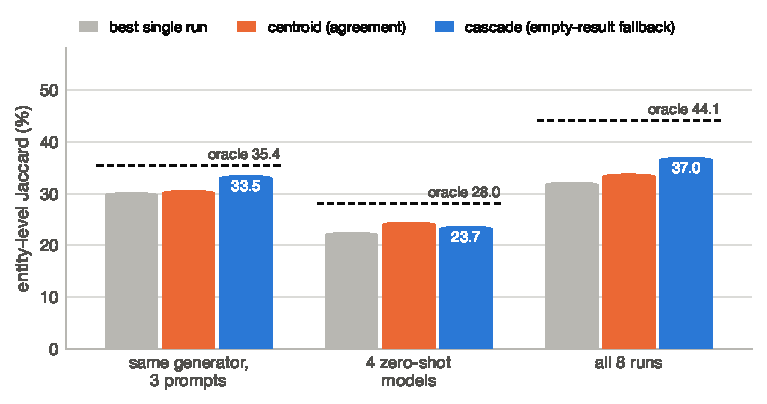
\includegraphics[width=0.88\textwidth]{figures/fig_cascade.pdf}
  \caption{Selection strategies over diverse generations.}
  \label{fig:cascade}
  \tabnote{Entity-level Jaccard. The dashed line represents the
oracle, which is an upper bound rather than an executable system. The
figures are based on the separate execution pass described in
this section and should not be directly compared with the
other tables in this chapter.}
\end{figure}

Selection by agreement does only slightly better than the individual runs: the result-set centroid reaches 33.8, against 37.0 for the cascade.
That does not mean agreement carries no useful information.
Candidates whose result sets agree with another candidate at 0.9 or above reach an average entity-level Jaccard of 43.8 against the reference, while candidates that agree with no other candidate reach only 13.3.

This information is largely redundant, however.
When several candidates agree, the preferred run is usually already among them.
When they disagree, the centroid often picks a plausible majority rather than the correct minority.
Where most candidates are wrong, checking whether the preferred query is valid is more useful than voting among all of them.

The results in this section come from a separate execution pass.
Its single-run scores are 0.8 to 1.4 points lower than the corresponding scores elsewhere in the chapter, because of endpoint state and the cap on returned values.
The comparisons within this section are internally consistent, but these figures should not be combined with the other tables.
The cascade order also uses knowledge of how good the runs are relative to each other.
The split-half analysis shows that the gain holds out of sample, but a deployed system would have to choose the order on a validation split.

\section{Benchmark Comparison and
Validity}

\subsection{Comparison with the Benchmark Authors'
Systems}

\label{sec:res-authors}

The benchmark authors publish generated queries for every test question under fourteen configurations.
Re-executing these stored outputs on the dump used here, with the same fair set and evaluation metric, allows a comparison free of additional inference variation, as shown in~\Cref{fig:frozen}.

\begin{figure}[htbp]
  \centering
  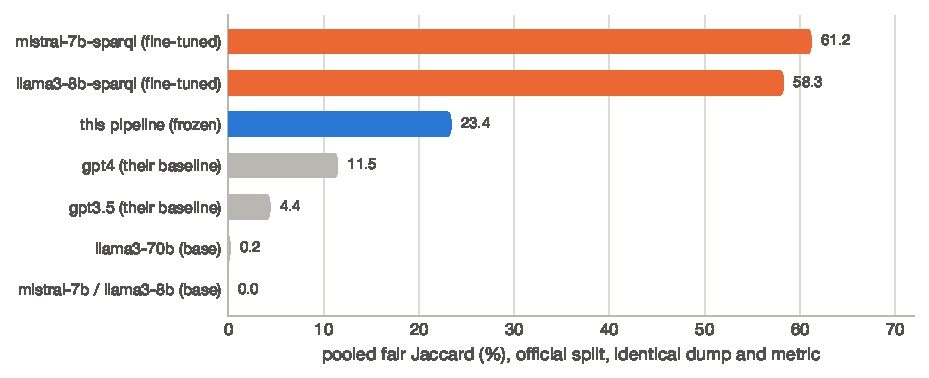
\includegraphics[width=0.88\textwidth]{figures/fig_frozen_vs_finetuned.pdf}
  \caption{Frozen and fine-tuned systems on the official split.}
  \label{fig:frozen}

\end{figure}

\emph{Figure note}.
All systems are evaluated on the same dump using the same strict fair set and metric.
The authors' results come from re-executing their published generated queries.

Every system is scored on all 370 strict-set questions of the official split, and a question for which a system produced no query counts as zero.
The fine-tuned models reach pooled fair Jaccard scores of 61.2 and 58.3, and the pipeline developed here reaches 23.4.
The authors' GPT-4 and GPT-3.5 baselines reach 11.5 and 4.4, respectively.
Without any in-domain training, the pipeline more than doubles the authors' frozen baselines and reaches more than one third of the fine-tuned systems' score.
Since its disambiguation is near-perfect, the remaining difference once more points to query generation.
This is a comparison between systems: the pipeline also uses a newer generator than the authors' GPT-4 baseline.
The pipeline's own contribution is measured on the working split, where it adds 6.0 pooled points over the same generator used zero-shot (19.1 to 25.1, \cref{tab:main}).

Of the best fine-tuned model's outputs, 56\,\% are character-identical to the reference query.
By contrast, exact and identifier-masked overlap between training and test queries is only 0.6\,\%, and the authors' training code loads the official training split.
This does not establish data leakage.
It rather suggests that fine-tuning teaches the model to reproduce the highly templated query style of the benchmark.
The benchmark was crawled from tutorial pages, and fine-tuning on 1,854 in-distribution queries exposes the model directly to this style.
A structural memorisation test indicates that the advantage extends beyond direct recall: accuracy is 55.1\,\% for rows whose structure closely matches a training query and 52.5\,\% for rows without such a match.

Base models without fine-tuning score at or near zero.
Llama 3 70B, for example, reaches only 0.2\,\% accuracy, with an execution rate of 14.2\,\%.
On this benchmark, the fine-tuned 7B model is roughly three hundred times more accurate than the base 70B model.
Model scale alone, it seems, does not replace what fine-tuning contributes.
One possible explanation is that fine-tuning improves conformity to the expected query idiom, the same capability that this chapter found lacking in the frozen models.

\subsection{Validity Checks}

\label{sec:res-validity}

\paragraph{Memorisation Check}

\begin{table}[htbp]
  \centering
  \caption{Structural similarity of generated queries to the benchmark.}
  \label{tab:memorisation}
  \small
  \resizebox{\ifdim\width>\textwidth\textwidth\else\width\fi}{!}{%
  \begin{tabular}{lrrrrrrrrrr}
    \toprule
    Run & n & Identical & $\geq$0.95 & $\geq$0.90 & Other, mean & Other $\geq$0.90 & Acc.\ close & Acc.\ other & n close & n other \\
    \midrule
    Zero-shot GPT-5.4 & 400 & 0.0 & 1.5 & 6.8 & 0.879 & 57.8 & 18.4 & 9.1 & 210 & 140 \\
    Zero-shot Claude & 400 & 0.0 & 1.2 & 7.5 & 0.9 & 66.0 & 23.2 & 18.0 & 249 & 106 \\
    Zero-shot Gemini & 400 & 0.2 & 2.2 & 11.2 & 0.91 & 67.8 & 10.8 & 7.6 & 238 & 104 \\
    Zero-shot DeepSeek & 398 & 0.0 & 1.0 & 6.8 & 0.847 & 47.5 & 13.5 & 11.6 & 170 & 174 \\
    Few-shot Claude & 400 & 0.0 & 2.2 & 9.8 & 0.918 & 74.2 & 24.7 & 14.5 & 276 & 81 \\
    End-to-end pipeline & 400 & 0.0 & 3.2 & 10.2 & 0.905 & 69.2 & 29.8 & 21.6 & 262 & 101 \\
    Idiom arm & 397 & 0.0 & 1.3 & 7.8 & 0.883 & 58.2 & 35.8 & 21.2 & 225 & 140 \\
    \bottomrule
  \end{tabular}}
  \tabnote{Skeletons compare query shape only: identifiers, literals, variable names, numbers and prefixes are removed. \emph{Identical} is the memorisation test; \emph{Other} measures resemblance to any other dataset query and reflects genericness rather than recall. For reference, 56\% of the benchmark authors' fine-tuned model's outputs are character-identical to the reference query. \emph{Identical}, $\geq$0.95 and $\geq$0.90 give the share of outputs (\%) whose skeleton is identical or that similar to its own reference; \emph{Other} is the best similarity to any other dataset query (mean, and share $\geq$0.90 in \%); \emph{Acc.} is entity-level Jaccard on rows whose structure is close ($\geq$0.90) to another dataset query and on the other rows.}
\end{table}


The Instruct-to-SPARQL dataset has been public since May 2025, while the models evaluated here were released in 2026 and their training data are undisclosed.
Memorisation is a real concern.
Recent work on LLM-generated SPARQL likewise shows that memorisation and externally injected graph knowledge can substantially affect apparent benchmark performance, which makes a direct check necessary~\citep{gashkov2025memorization}.
The check uses the same skeleton comparison as the earlier analysis: identifiers, literals, variable names, numbers and prefixes are removed, leaving only the query structure.

No frozen run reproduces the reference structures to any substantial degree.
Between 0.0\,\% and 0.2\,\% of outputs are skeleton-identical to their own reference query, and 1.0\,\% to 3.2\,\% reach a similarity of at least 0.95.
This contrasts with the 56\,\% of character-identical outputs reported for the benchmark authors' fine-tuned model.
\Cref{fig:memorisation} and~\cref{tab:memorisation} report the distributions.

The figure also includes a measure that could be mistaken for evidence of copying.
Between 47.5\,\% and 74.2\,\% of generated skeletons have at least 0.90 similarity to some other query in the dataset.
This does not necessarily indicate memorisation.
Generated skeletons are often simple, and simple structures naturally resemble many other queries.
The rate is also higher than the 36.5\,\% similarity rate among the reference queries themselves.

Structural simplicity likewise explains the apparent accuracy advantage on questions that are structurally close to known queries.
Within complexity groups, the difference shrinks or disappears: zero-shot Claude, for example, scores 23 versus 22 on medium questions and 19 versus 16 on complex ones.
The test detects structural reproduction, not memorisation of a complete mapping from question to answer.

\paragraph{Representativeness of the Benchmark}

\begin{table}[htbp]
  \centering
  \caption{Construct prevalence: benchmark gold queries versus real query logs.}
  \label{tab:wdql}
  \small
  \resizebox{\ifdim\width>\textwidth\textwidth\else\width\fi}{!}{%
  \begin{tabular}{llrr}
    \toprule
    Queries & Construct & Benchmark (\%) & WDQL (\%) \\
    \midrule
    all & subclass closure (P279*) & 23.6 & 12.8 \\
     & statement node (p:) & 23.1 & 6.7 \\
     & qualifier (pq:) & 15.1 & 3.8 \\
     & value node (psv:/psn:) & 6.1 & 0.8 \\
     & aggregation (GROUP BY) & 31.9 & 11.5 \\
     & alternation (VALUES/UNION) & 17.3 & 12.8 \\
     & property path (/ | * +) & 38.8 & 16.8 \\
     & OPTIONAL & 39.9 & 29.8 \\
     & FILTER & 36.2 & 59.6 \\
     & LIMIT & 10.8 & 26.0 \\
     & any reification or hierarchy idiom & 41.2 & 18.8 \\
    \midrule
    5+ predicate tokens & subclass closure (P279*) & 31.6 & 25.6 \\
     & statement node (p:) & 37.4 & 18.9 \\
     & qualifier (pq:) & 24.7 & 13.1 \\
     & value node (psv:/psn:) & 11.3 & 3.3 \\
     & aggregation (GROUP BY) & 33.6 & 15.7 \\
     & alternation (VALUES/UNION) & 24.8 & 21.8 \\
     & property path (/ | * +) & 53.6 & 34.9 \\
     & OPTIONAL & 53.6 & 53.9 \\
     & FILTER & 46.9 & 83.6 \\
     & LIMIT & 10.3 & 33.7 \\
     & any reification or hierarchy idiom & 58.8 & 41.2 \\
    \bottomrule
  \end{tabular}}
  \tabnote{WDQL is the Wikidata Query Logs dataset (one-per-cluster release, 226{,}376 real queries). Size bands are predicate-token counts, a formatting-robust proxy for triple patterns. Counts: 2{,}838 benchmark and 226{,}376 WDQL queries in all; 1{,}525 and 51{,}728 with 5+ predicate tokens.}
\end{table}


The main findings concern query constructs measured on a benchmark collected from tutorial pages.
Whether these constructs also matter in everyday Wikidata use is a separate question.
To answer it, the benchmark is compared with the Wikidata Query Logs dataset~\parencite{walter2026wdql}, which contains 226,376 real queries sent to the public query service.

Across all queries, the benchmark contains substantially more reification and hierarchy idioms.
At least one such construct appears in 41.2\,\% of benchmark reference queries, against 18.8\,\% of query-log queries (\cref{fig:wdql}).
Benchmark queries are, however, generally larger, so query size affects this comparison.

When both datasets are restricted to queries with at least five predicate tokens (\cref{fig:wdql-size}), the difference shrinks but remains visible:

\begin{itemize}
\item
Any reification or hierarchy idiom: 58.8\,\% versus 41.2\,\%
\item
Subclass closure: 31.6\,\% versus 25.6\,\%
\item
Statement nodes: 37.4\,\% versus 18.9\,\%
\item
Value nodes: 11.3\,\% versus 3.3\,\%
\end{itemize}

\begin{figure}[htbp]
  \centering
  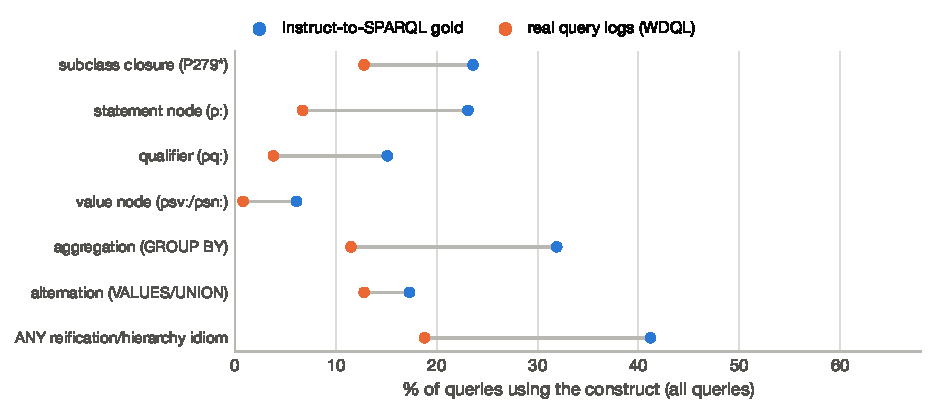
\includegraphics[width=0.88\textwidth]{figures/fig_wdql.pdf}
  \caption{Construct prevalence: benchmark gold queries against real Wikidata query logs.}
  \label{fig:wdql}
  \tabnote{The comparison includes all queries in both datasets.
Benchmark queries are larger on average, which confounds the comparison.
\cref{fig:wdql-size} controls for query size.}
\end{figure}

The relevant idioms are not just artefacts of the benchmark: roughly two in five non-trivial queries use at least one of them, so a system that cannot generate them will fail on a substantial share of real Wikidata queries.
The benchmark does, however, over-represent these constructs.
At matched query sizes, they are about 1.2 to 2 times more frequent in the benchmark, and value nodes around 3.4 times.
The accuracy reported here may therefore underestimate performance on questions distributed more like real query logs.

The comparison has limits of its own.
The query-log questions were generated by a model.
The logs also date from 2017--2018 and include bot traffic, which may explain the relatively high frequency of FILTER and LIMIT clauses.

\chapter{Discussion}

\label{ch:discussion}

This chapter interprets the results research question by research question, then turns to the measurement artefacts identified during the study and to the scope of the findings.

\section{Main Findings}

\paragraph{RQ1: What Frozen Frontier Models Can and Cannot
Do}

\label{sec:disc-rq1}

Frozen frontier models write SPARQL that parses and executes but is rarely correct (\cref{sec:res-frozen}, \cref{tab:main}).
On non-empty outputs their scores lie close together.
What separates the systems is mainly how often they return nothing, and the pipeline roughly halves that rate.
Their weakness lies in Wikidata's modelling conventions (statement nodes, subclass closure, normalised value nodes), which they rarely apply where needed.

The failures are shared across models.
Three quarters of the questions are solved by none of the four models, which come from four different organisations.
The questions that all four fail share a clear feature in their reference queries: they contain several times more statement nodes than easier questions, and qualifier access and aggregation, which appear in them, never occur in the questions that all four models solve.
This suggests that the difficulty is a property of the questions themselves.

Fine-tuning brings conformity to a query style, the very capability the frozen models lack: a 7B model trained on in-domain queries scores orders of magnitude higher than a much larger base model.
This does not prove a general difference in capability, since more than half of its outputs are character-identical to the reference, although that alone does not establish leakage.
A fine-tuned system reproduces a distribution of queries, whereas this pipeline derives a query from the question. The two agree only when the reference translates the question correctly, but the audit shows noise in roughly one quarter of the strict fair set.
Whether this contributes materially to the observed gap remains open, since only sixteen adjudicated rows overlap the official split, and it is listed as future work.

The comparison that matters most for this thesis is among systems without in-domain training, and there the pipeline more than doubles the best published frozen result.
The stage-wise analysis also shows where the remaining difference to fine-tuned systems comes from.

\paragraph{RQ2: Why Disambiguation Is Not the
Bottleneck}

\label{sec:disc-rq2}

Given the benchmark's concepts and query structure, the pipeline reaches 97.4 entity-level Jaccard (\cref{sec:res-attribution}, \cref{tab:main}).
When it has to generate the query itself, the score falls to 30.9.
In this pipeline, query generation is the main constraint.
Disambiguation over retrieved candidates stops being the limiting stage once the model writes suitable labels and the correct entity is in the candidate pool, which holds for the frontier model here.
For the small open model, label generation itself becomes the weak point (see RQ3).

Rebuilding the candidate pools with rate-limited retrieval adds further support: the gold-label condition improved roughly ten times more than the end-to-end condition, which is hard to explain if disambiguation were the main constraint.

Structure is the largest single component of the gap and dominates at high complexity, but it is not the only source of error: projection mismatches and residual identifier errors each account for about one fifth of the failures.
Within generation, the factorial arm separates the two decisions: fixing the concepts is worth +19.72 points and naming the required idioms +3.76, and the two effects add up.
Even with both supplied, the model reaches 50.4 against 97.4 for the gold-label condition, so composing the query around the right concepts remains the largest single step.

\paragraph{Performance of the End-to-End Linkers}

The fine-tuned linkers' deficit of about 70 points traces to the mention-detection mismatch discussed in the related work, and the set-based metric closes only a small part of it.
Given the same candidates, the bi-encoder trails the reasoning linker by 24.9 points and the plain search order by about 21, so reasoning over candidates is the strongest of the compared mechanisms, while most of its accuracy comes from labels that Wikidata's search can find.
Research that focuses mainly on entity linking for this task, including the 35.1\,\% failure share reported by \citet{xu2023wikisp}, may therefore be improving a stage that this architecture has largely solved.
\citet{xu2023wikisp} measured a fine-tuned system on simpler questions, where linking makes up a larger share of the errors; the two results describe different architectures and do not contradict each other.
For a pipeline of this kind, better disambiguation offers little headroom, while query generation leaves much more room.

\paragraph{RQ3: What Backbone Scale Buys, and
Where}

\label{sec:disc-rq3}

Backbone dependence differs by stage (\cref{sec:res-linkers,sec:res-backbone}, \cref{tab:linkers}).
At disambiguation, scale has little effect: 97.7 (frontier), 94.9 (14B) and 95.8 (7B) entity F1, with overlapping intervals.
Reasoning over seven retrieved candidates does not need a frontier-scale model.
At generation, however, the choice of backbone matters much more: when the open model handles both stages, pipeline performance drops sharply.

Asked to name Wikidata entities and properties without further help, the open model produces unfindable labels for 16.4\,\% of distinct labels (270 of 1,645), against 3.3\,\% for the frontier model, a 4.9-fold difference.
This points to a hybrid deployment, with a capable model for labels and a cheaper one for disambiguation.
String normalisation, which should fix superficial casing issues such as camelCase or snake\_case, lowers the failure rate only to 13.8\,\%.
The main problem is near-miss wording (``crew member(s)'', for example, names a different property and is not a misspelling), and normalisation hardly touches it.
The replication with Claude Opus 5 repeats generation with a later frontier model and finds the same pattern: subclass closure and property paths improve, statement nodes and qualifiers improve little, and value nodes do not improve.
The generation deficit does not disappear as models get better.
Schema evidence, selective gating, majority voting and string repair fail in the same way: none of them supplies knowledge of how the graph itself names and models information.
The disambiguation results show that the smaller model already reasons well enough for that stage, so the most likely explanation for the generation gap is missing vocabulary knowledge.

\paragraph{RQ4: Guidance versus
Evidence}

\label{sec:disc-rq4}

Generic idiom guidance brings a small benefit (\cref{sec:res-prompts}, \cref{tab:significance}), evidence about graph contents does about four times as much harm, and selective guidance does not beat always-on guidance, even with oracle knowledge of when it is needed.

\paragraph{Overuse of Schema Evidence}

When the model is shown the properties of an entity, it uses them about twice as often as the reference does.
Making the evidence shorter and explicitly conditional does not reduce this overuse but increases it.
The grounded arms share only half as much label vocabulary with the baseline as the idiom arm does.
The intervention failed even though the schema cards were built from reference-linked mentions, with no linking errors at all.

\paragraph{Predicting Construct Need from the Question}

A classifier that predicts from the question text alone whether a reference query uses a given construct reaches only moderate performance (AUC 0.62--0.82).
Its strongest features for subclass closure are topical terms (``libraries'', ``hospitals'', ``scientists''), which describe the subject of a question, not how Wikidata models it.

\paragraph{Cost of Unnecessary Idiom Use}

The idiom prompt helps most when the reference needs the construct it describes, and on average it still raises accuracy when it does not, although individual questions can get worse.
Unnecessary closure over a class without subclasses simply returns the same rows.
Construct predictions are miscalibrated, but the cost in accuracy is small, so selective application addresses a problem that is usually cheap.

\paragraph{Constraining versus Enumerating the Schema}

The contrast with \citet{zhang2026saga} helps explain the schema-evidence result.
SAGA filters candidates by type, domain and range, removing options that would otherwise be chosen wrongly.
The schema-evidence arm does the opposite and adds options, which the model seems to take as encouragement.
The same graph information has opposite effects, depending on whether it filters or merely informs.
This also explains why linking (seven candidates, a forced choice) does better than grounding (everything an entity carries, with no restriction).
The direction of the knowledge mattered more than its amount: narrowing the decision space helped, and widening it hurt.
The same distinction sets this result apart from \citet{yang2026ggc}, whose gate reduces the cost of an expensive and often harmful operation.
The gate tested here would have to improve accuracy for an operation that is cheap and almost never harmful, so there is no comparable gain for gating to find.

\paragraph{Testing the Principle}

The prompt experiment keeps the same reference-linked information and changes only how it is presented.
Offered as available evidence, it lowers performance by 14.65 points.
Imposed as a mandatory closed list, it raises performance by 18.99 points.
The intervals do not overlap, which leaves a difference of about 34 points from framing alone.
The absolute level is partly definitional, because the permitted list is drawn from the reference query's own vocabulary, so the evidence lies in the contrast between the two framings.
The model broke the prompt-level constraint for only 0.7\,\% of label uses.

The mechanical half of the principle was tested separately.
Applying every type constraint declared in Wikidata removes the reference property for 7.5\,\% of the affected mentions, while using only mandatory constraints is safe but has almost no effect.
The principle still holds, since constraining beats enumerating.
A mechanical filter, however, is only as reliable as Wikidata's own assertions, and most declared type constraints are not binding.

\paragraph{What the Interventions Changed}

The constrained arm gains more than the construct-profile arm, because it settles concept selection, the larger of the two generation decisions it can address.
The factorial arm shows that the two contributions add up, and naming a construct is still not the same as providing the composed query.
The profile hint tells the model which idiom a question needs, but it does not show how to build a complete query around it.
General advice brought no further gains in these experiments.
Restricting the identifiers available to the generator was the more effective intervention.

\paragraph{RQ5: Detectable Failure and the Value of
Execution}

\label{sec:disc-rq5}

Some failures can be detected without the gold query (\cref{sec:res-cascade}, \cref{tab:cascade}).
A cascade that accepts the first non-empty, error-free result raises the score by +4.83 points [2.93, 7.08] without any additional training.
Because it only replaces empty or failed results, it cannot worsen a question by design.
Of the 92 fallback rows, 64 are triggered by empty results.
The gain amounts to about two fifths of the 12-point oracle headroom, so execution feedback catches some failures but cannot correct a query that runs successfully and returns the wrong answer.

The cascade also beats result-set majority voting (37.0 vs.\ 33.8 for the centroid, against a 32.2 baseline): agreement between outputs is a weaker signal than execution, because wrong queries can agree with each other.
Unlike agentic self-correction, which generates, executes and revises queries in a loop, the cascade checks existing alternatives in a fixed order.
This makes it cheaper and easier to reproduce.
It recovers a failure whenever one of the alternatives is correct.
Generating the correct structure in the first place remains the main direction for future work.

\section{Methodological
Implications}

\label{sec:disc-artefacts}

Four measurement artefacts arose during the study, each producing a plausible but incorrect intermediate result.
All four were detected and corrected before the final analysis and are documented in the appendix.
Their causes differed, but they had one feature in common: the result was plausible and fitted the emerging interpretation.

\begin{table}[htbp]
\centering
\small
\caption{Four measurement artefacts: the apparent result and the correction.}
\label{tab:artefacts}
\begin{tabular}{@{}p{3.1cm}p{4.6cm}p{5.6cm}@{}}
\toprule
Artefact & Apparent result & Correction \\
\midrule
Jaccard(\(\emptyset\),\(\emptyset\)) = 1 & Inflated the score of systems that returned nothing & Strict fair set requires a non-empty reference \\
Silent API throttling & An 80.4\,\% candidate ceiling read as a retrieval bottleneck & Rate-limited, repaired pools raised the ceiling to 99.4\,\% \\
Exceptions caught as empty strings & A reported 66.8\,\% generation-success rate on complex questions & Every affected row succeeded on regeneration \\
A stale error sample & Complex failures judged to contain no linking errors & The correct run contained three linking errors among fifteen \\
\bottomrule
\end{tabular}
\end{table}

The lesson is that a plausible result needs more than a check of the final score: these artefacts were caught through regeneration, auditing and comparison with intermediate outputs.
In practice, empty or unusually short responses from the Wikidata search API should be treated as suspicious and re-checked with repeated requests, and KGQA experiments should be regenerated end to end from stored inputs after any change to the pipeline.

\begin{figure}[htbp]
  \centering
  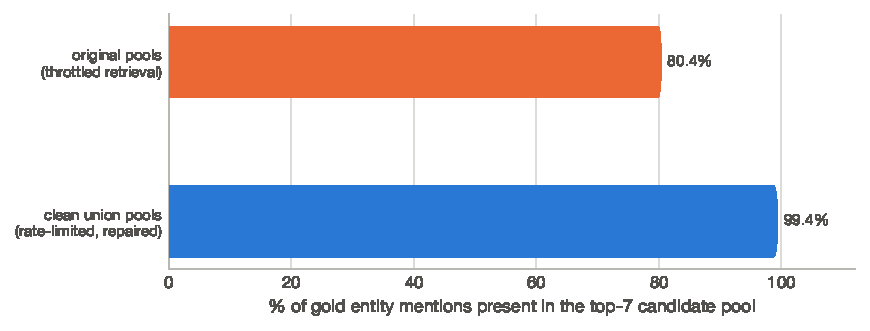
\includegraphics[width=0.88\textwidth]{figures/fig_candidate_ceiling.pdf}
  \caption{A measurement artefact: the candidate ceiling before and after pool repair.}
  \label{fig:ceiling}

\end{figure}

\emph{Figure note}.
The initial 80.4\,\% ceiling was caused by silent API throttling.
The issue came to light through rank analysis and through the implausibly large improvement after the pools were repaired.

\section{Limitations and Scope}

\label{sec:limitations}

\begin{enumerate}
\def\labelenumi{\arabic{enumi}.}
\item
\textbf{Evaluation asymmetry.}
The reasoning linkers and GLiNKER receive mention strings and curated candidate lists, whereas ELQ and ReFinED have to detect mentions themselves.
The set-based metric closes part of this gap (+5.4 and +6.8 points), and GLiNKER is evaluated on the reasoning linker's candidate lists rather than with its own retrieval.
\item
\textbf{Benchmark validity.}
Reference noise affects an estimated 24.6\,\% of the strict fair set (interval [12.9, 42.0]).
Scores are not corrected for it, so that they remain comparable with the existing literature.
\item
\textbf{Scope.}
The study evaluates four models from four organisations and two frontier generations in an English setting, on one Wikidata dump served by QLever, which excludes around 15\,\% of gold queries that depend on Blazegraph-specific behaviour.
The linking results are replicated on LC-QuAD 2.0, while the structural gap is measured on Instruct-to-SPARQL.
The design principle of constraining rather than enumerating the schema is established on one benchmark, one generation backbone and one schema-card design.
\item
\textbf{Oracle interventions.}
The constrained-vocabulary and construct-profile arms draw their information from the reference query, and the permitted list can also hint at structure, for example when it contains a qualifier property.
\item
\textbf{Cascade assumptions.}
The cascade never lowers accuracy on the strict fair set because every reference returns a result.
Where an empty answer can be correct, an empty result is not always a failure.
Its prompt order was chosen from the relative quality of the runs, and the split-half evaluation shows that the gain holds when the order is chosen on other questions.
\item
\textbf{Sample size of the error analysis.}
The error taxonomy covers 30 failures and identifies recurring types rather than population frequencies.
The corpus-wide construct analysis across all 567 rows supports the same conclusion.
\end{enumerate}

\chapter{Conclusion}

\label{ch:conclusion}

\section{Summary}

\label{sec:conclusion-summary}

This thesis examined where a frozen-model text-to-SPARQL pipeline over Wikidata fails and whether targeted interventions can reduce those failures.
It uses \method{}, which keeps every stage fixed except the one under investigation and evaluates that stage on its own.
\Cref{tab:conclusion-summary} collects the headline figures for each research question.
The paragraphs below state the findings, and the results and discussion chapters give the full evidence and its limits.

\begin{table}[htbp]
\centering
\small
\caption{Findings by research question. Evidence, intervals, caveats are in Results and Discussion.}
\label{tab:conclusion-summary}
\begin{tabular}{@{}p{0.9cm}p{7.6cm}p{4.4cm}@{}}
\toprule
RQ & Finding & Key figures \\
\midrule
1 & Frozen models parse and execute reliably but are rarely correct; failures are shared across models & 24.5 best frozen baseline; 307/400 solved by none of four models \\
2 & Under gold labels and near-ceiling candidate coverage, disambiguation is not the binding constraint; query generation is & 97.4 gold-label vs.\ 30.9 end-to-end (66.5-pt gap) \\
3 & Reasoning over retrieved candidates outperforms specialised linkers; most of its accuracy comes from findable labels & +24.9 [22.3, 27.7] pts over GLiNKER on the same candidates; +4.1 [2.7, 5.6] over the first search result \\
4 & General advice gives small gains; graph knowledge helps as a restriction, not as evidence & $-$14.65 pts (evidence) vs.\ $+$18.99 pts (closed vocabulary) \\
5 & Some failures are detectable from execution alone, without gold supervision & +4.83 [2.93, 7.08] pts; no row can worsen by design \\
\bottomrule
\end{tabular}
\end{table}

\paragraph{RQ1.}

Frozen frontier models write SPARQL that executes but is rarely correct, and their failures are shared across models.

\paragraph{RQ2.}

With gold-derived labels and near-ceiling candidate coverage, the binding constraint is query generation, not disambiguation.
Supplying the concepts helps more than naming the constructs, but composing the query around them remains the largest step: with both supplied, accuracy is 50.4 against 97.4 when the composed reference query is given.

\paragraph{RQ3.}

Reasoning over retrieved candidates clearly outperforms specialised end-to-end linkers, and evaluation asymmetry alone does not explain the gap.
Disambiguation hardly depends on the backbone, while label generation does.

\paragraph{RQ4.}

General advice gives small gains, and graph knowledge helps when it restricts the generator's choices.

\paragraph{RQ5.}

Some of the remaining failures can be detected from execution alone, without gold supervision.
The execution-guided cascade recovers about two fifths of the available oracle headroom.

Together, these findings yield a working pipeline in which every step is chosen on experimental evidence, and a protocol for finding where such pipelines fail.

\section{The Resulting System}

\label{sec:conclusion-system}

The measurements settle several design choices that are often made by convention, and together they describe a configuration that others can start from.

Label generation needed the strongest model, while for disambiguation an open 7B model came within two points of it (95.8 against 97.7 entity F1).
Scale matters at only one stage: the 14B open model produces unfindable labels at 4.9 times the frontier rate, whereas disambiguation varies by less than three percentage points across model sizes.

For linking, retrieving candidates and reasoning over them worked better than linking end to end.
Both fine-tuned linkers fail mainly because they detect mentions in the question text and therefore miss identifiers that the question never names (\cref{sec:res-linkers}).
On a second benchmark, reasoning over candidates again links entities accurately (90.6\,\% entity accuracy), so the result is not specific to one dataset.

Constrain the vocabulary; do not enumerate the schema.
In this pipeline, graph knowledge supplied before generation helped only when it removed options.

An empty result is a useful signal at inference time, because structurally wrong queries often return nothing.
The cascade built on this signal requires no training or gold answers, only replaces failed queries, and should be the baseline for any learned selector.

Candidate pools need to be checked before any linking number can be trusted.
Fixing silently truncated pools raised the gold-label condition by 26 points, because a retrieval layer that returns an empty list because of throttling looks exactly like one that returns an empty list because nothing matches.

The open problem is building a query around a construct that the model can identify but does not yet use correctly.
The next section describes the research directions that follow from this.

\section{Future Work}

\label{sec:future-work}

\paragraph{Grounding by constraint through
filtering.}

The prompt experiment here tests the framing side of this principle at the prompt level, whereas \citet{zhang2026saga} remove incompatible candidates mechanically.
Such filtering replaces the model's obedience with the reliability of Wikidata's own assertions.
The constraint-filtering experiment shows, however, that these assertions can be weak: filtering on every declared type constraint removes the reference property for 7.5\,\% of the mentions it affects, while filtering only on mandatory constraints is safe but does almost nothing.
Whether the safe filter improves accuracy is still open.

\paragraph{Closing the open model's vocabulary
gap.}

String normalisation is not enough: it repairs 43 of 270 unfindable labels, because the main problem is often a different property name rather than a malformed one.
Supplying the vocabulary through constrained generation or light adaptation could make the hybrid deployment discussed earlier unnecessary.

\paragraph{A learned selector over diverse
generations.}

About seven points of oracle headroom remain beyond the cascade.
A learned selector should therefore be evaluated against the cascade, not only against the best single run.

\paragraph{Extending the ground-truth
derivation.}

The linking ground-truth derivation used here needs only aligned gold and label-form queries.
LC-QuAD 2.0~\parencite{dubey2019lcquad2} was used here only to replicate the linking measurement; a full stage-wise analysis on it, including the structural gap, would show whether the attribution holds beyond Instruct-to-SPARQL.
The Wikidata Query Logs dataset~\parencite{walter2026wdql} would test whether it holds for questions distributed like real query logs.

\paragraph{Assessing whether reference noise favours imitation over reasoning}

The discussion identified a mechanism worth testing directly: a fine-tuned system reproduces reference queries (56\,\% character-identical), so an unsound reference rewards imitation over reasoning, and part of the measured gap may come from the answer key itself.
Testing this requires extending the reference-query adjudication to the official split, since nine overlapping rows are not enough.

\paragraph{Re-adjudicating the benchmark's reference
queries.}

Given the 24.6\,\% reference-noise estimate, a large-scale correction should judge the query text rather than the executed output, use two readers with reconciliation, and also sample queries that a heuristic did not flag, since every correction in this study came from that group.

\runningbodychaptersfalse

{\setstretch{1.0}\printbibliography[heading=bibintoc,title={References}]}

\appendix
\chapter{Appendix}
\label{ch:appendix}

\section{Prompts}
\label{app:prompts}

The prompt-intervention experiment changes only the generation prompt, so the prompts are reproduced below.
The prompts are reproduced exactly as used in the experiments.

The baseline arm uses~\cref{lst:prompt-gen} alone.
The idiom arm uses the base system prompt followed by the idiom guide (\cref{lst:prompt-idiom}).
The two schema-evidence arms append a per-question schema card, and \cref{lst:schema-cards} shows one card of each form; the code that builds the cards is in the accompanying repository.
Disambiguation (\cref{lst:prompt-disamb}) is identical in every arm.

\begin{lstlisting}[caption={Generation system prompt (baseline).},label={lst:prompt-gen},basicstyle=\ttfamily\scriptsize,breaklines=true,captionpos=b]
You are a SPARQL expert for Wikidata. Generate a SPARQL query that
answers the question, but instead of using opaque Wikidata IDs, use human-readable
labels in this exact bracket format:
  - For entities:   wd:[entity:LABEL]      e.g. wd:[entity:Christopher Nolan]
  - For properties: wdt:[property:LABEL]   e.g. wdt:[property:director]
Use this format for ALL entities and properties. Keep variable names and SPARQL
structure normal. Output ONLY the SPARQL query, no explanation.
\end{lstlisting}

\begin{lstlisting}[caption={Disambiguation prompt, as built by the pipeline. The candidate list is injected at \texttt{\{cand\_text\}}. The reported runs send this prompt through Anthropic's batch interface or, for the open models, through vLLM. If the answer contains no identifier, or a request fails, the first search result is used instead; in the reported frontier-model runs all 4,063 requests returned an answer line, so this fallback was never used.},label={lst:prompt-disamb},basicstyle=\ttfamily\scriptsize,breaklines=true,captionpos=b]
def disambiguate(question, label, candidates, is_property=False):
    if not candidates:
        return ""
    if len(candidates) == 1:
        return candidates[0]["id"]
    kind = "property" if is_property else "entity"
    cand_text = "\n".join(
        f"  {c['id']}: {c['label']} — {c['description'] or '(no description)'}"
        for c in candidates)
    example_id = "P57" if is_property else "Q25191"
    prompt = f"""Question: "{question}"

Find the correct Wikidata {kind} ID for: "{label}"

Candidates:
{cand_text}

Think step by step about which candidate best fits the {kind} "{label}" in the
context of the question. Output ONLY the chosen ID (e.g. {example_id}) on the last
line, prefixed with "ANSWER: ".
"""
\end{lstlisting}

\begin{lstlisting}[caption={Idiom-guidance prompt. The idiom arm is \textsc{base} followed by \textsc{idiom guide}; the baseline arm is \textsc{base} alone.},label={lst:prompt-idiom},basicstyle=\ttfamily\scriptsize,breaklines=true,captionpos=b]
You are a SPARQL expert for Wikidata. Generate a SPARQL query that
answers the question, but instead of using opaque Wikidata IDs, use human-readable
labels in this exact bracket format:
  - For entities:   wd:[entity:LABEL]      e.g. wd:[entity:Christopher Nolan]
  - For properties: wdt:[property:LABEL]   e.g. wdt:[property:director]
Use this format for ALL entities and properties. Keep variable names and SPARQL
structure normal. Output ONLY the SPARQL query, no explanation.

Before writing the query, consider which of Wikidata's modelling idioms the
question requires. Use them where appropriate:

1. Class membership is usually hierarchical. A question about a category
   normally means the category and all of its subclasses, so prefer
   ?item wdt:[property:instance of]/wdt:[property:subclass of]* wd:[entity:CLASS]
   over a direct instance-of triple. Use the direct form only when the question
   clearly means the class itself.

2. Values that carry extra information live on statements, not on direct
   claims. When the question asks about a qualifier — a date, a rank, a role, a
   plot, a part something applies to — go through the statement node:
     ?item p:[property:P] ?st .
     ?st ps:[property:P] ?value ; pq:[property:QUALIFIER] ?qvalue .
   Direct wdt: triples cannot see qualifiers.

3. Quantities with units, precision or bounds require the statement value node:
     ?item p:[property:P]/psv:[property:P] ?vn .
     ?vn wikibase:quantityAmount ?amount ; wikibase:quantityUnit ?unit .
   Use this whenever units must be compared or converted.

4. Questions about words, forms, senses or languages concern lexemes, not
   items: use wikibase:lemma, dct:language, ontolex:sense and the lexeme
   namespace rather than item properties.

5. Counting, ranking or "how many / most / per X" questions need explicit
   aggregation: COUNT/SUM with GROUP BY, and ORDER BY ... DESC for ranking.

6. Alternatives in the question ("mathematicians or physicists", several
   platforms) are expressed with VALUES or UNION, not by choosing one.

7. Do not add LIMIT unless the question asks for a specific number of results.

Apply only the idioms the question actually calls for; do not add machinery
that is not needed.
\end{lstlisting}

\begin{lstlisting}[caption={Schema-card construction: the first function produces the verbose arm's evidence and the second the targeted arm's.},label={lst:prompt-schema},basicstyle=\ttfamily\scriptsize,breaklines=true,captionpos=b]
def build_card(entities, properties, prop_cache, ent_cache):
    """Compose the compact evidence text placed in the generation prompt.
    Entity evidence is included when the question mentions entities; property
    evidence is always included, so property-only questions are covered too."""
    lines = []
    for qid in entities[:MAX_ENTS]:
        info = ent_cache.get(qid)
        if not info:
            continue
        head = f"{qid} ({info['label']})"
        if info["is_class"]:
            head += " — this is a class with subclasses; a question about it " \
                    "usually means the class and everything below it"
        lines.append(head)
        if info["properties"]:
            named = ", ".join(f"{p} ({prop_cache.get(p, {}).get('label', p)})"
                              for p in info["properties"][:MAX_PROPS])
            lines.append(f"  properties in use: {named}")
        if info["qualified"]:
            named = ", ".join(f"{p} ({prop_cache.get(p, {}).get('label', p)})"
                              for p in info["qualified"][:8])
            lines.append(f"  statements with qualifiers (need p:/pq: to read "
                         f"the qualifier): {named}")
        quants = [p for p in info["properties"]
                  if prop_cache.get(p, {}).get("quantity")]
        if quants:
            lines.append(f"  quantity-valued (unit lives on the value node, "
                         f"need p:/psv:): {', '.join(quants[:6])}")

    prop_lines = []
    for pid in properties[:MAX_PROPS]:
        info = prop_cache.get(pid)
        if not info:
            continue
        bits = []
        if info.get("qualifiers"):
            named = ", ".join(f"{q} ({prop_cache.get(q, {}).get('label', q)})"
                              for q in info["qualifiers"][:5])
            bits.append(f"used with qualifiers {named}, reachable only through "
                        f"p:/pq:")
        if info.get("quantity"):
            bits.append("quantity-valued; the unit sits on the statement value "
                        "node, reachable through p:/psv:")
        if info.get("class_range"):
            bits.append("its values are classes with subclasses, so filtering "
                        "on one usually needs P279* closure")
        if bits:
            prop_lines.append(f"{pid} ({info.get('label', pid)}): " + "; ".join(bits))
    if prop_lines:
        lines.append("properties this question refers to:")
        lines += ["  " + l for l in prop_lines]
    return "\n".join(lines)

def build_card_targeted(entities, properties, prop_cache, ent_cache):
    """Targeted variant: evidence ONLY for the properties/entities the
    question actually links to (gold mentions), no enumeration of everything
    an entity happens to carry. Tests whether the full-listing version failed
    from information overload/distraction rather than from the concept of
    grounding itself."""
    lines = []
    for qid in entities[:MAX_ENTS]:
        info = ent_cache.get(qid)
        if info and info.get("is_class"):
            lines.append(f"{qid} ({info['label']}) is a class with subclasses: "
                         f"a question about it usually means the class and "
                         f"everything below it (wdt:[property:instance of]/"
                         f"wdt:[property:subclass of]*).")
    seen = set()
    for pid in properties[:MAX_PROPS]:
        info = prop_cache.get(pid)
        if not info or pid in seen:
            continue
        seen.add(pid)
        label = info.get("label", pid)
        bits = []
        if info.get("qualifiers"):
            bits.append("if the question asks for something beyond the plain "
                        "value (e.g. a date, role or extra detail attached to "
                        "this fact), it is recorded as a QUALIFIER and needs "
                        "p:[property:" + label + "] / pq:[property:...], not "
                        "wdt:[property:" + label + "] alone")
        if info.get("quantity"):
            bits.append("its value is a QUANTITY with a unit; if the unit or "
                        "precision matters, use p:/psv: to reach the value node")
        if info.get("class_range"):
            bits.append("its value is itself a class; if the question means "
                        "the value or anything below it, add "
                        "wdt:[property:subclass of]* on the value")
        if bits:
            lines.append(f"{pid} ({label}): " + "; ".join(bits) + ".")
    return "\n".join(lines)
\end{lstlisting}

\begin{lstlisting}[caption={Example schema cards, one of each form, as supplied to the generator.},label={lst:schema-cards},basicstyle=\ttfamily\scriptsize,breaklines=true,captionpos=b]
--- verbose card (row 0) ---
properties this question refers to:
  P625 (coordinate location): used with qualifiers P2241 (reason for deprecated rank), P459 (determination method or standard), P518 (applies to part), P609 (terminus location), P813 (retrieved), reachable only through p:/pq:

--- targeted card (row 0) ---
P625 (coordinate location): if the question asks for something beyond the plain value (e.g. a date, role or extra detail attached to this fact), it is recorded as a QUALIFIER and needs p:[property:coordinate location] / pq:[property:...], not wdt:[property:coordinate location] alone.
\end{lstlisting}


\section{Full Result Tables}
\label{app:tables}

The results chapter reports the main comparisons on the common subset. The tables below provide the full results, including per-run denominators, complexity breakdowns, and confidence intervals.
The tables below provide the full results with per-run denominators, breakdowns by complexity, and complete interval estimates.

\begin{table}[htbp]
\centering
\footnotesize
\caption{Full strict-set results with per-run denominators, working split.}
\label{tab:app-master}
\resizebox{\ifdim\width>\textwidth\textwidth\else\width\fi}{!}{%
\begin{tabular}{@{}lrrrrrrr@{}}
\toprule
Approach & Questions scored & Pooled (\%) & Simple & Medium & Complex & Entity-level (\%) & Entity rows \\ \midrule
Zero-shot GPT-5.4 & 400 & 12.8 & 21.7 & 13.1 & 10.7 & 14.7 & 350 \\
Zero-shot Claude Opus 4.8 & 400 & 17.8 & 29.7 & 18.8 & 14.2 & 21.7 & 355 \\
Zero-shot Gemini 3.1 Flash Lite & 400 & 8.6 & 13.9 & 10.4 & 5.4 & 9.8 & 342 \\
Zero-shot DeepSeek V4 Flash & 400 & 10.4 & 21.2 & 11.2 & 7.4 & 12.5 & 346 \\
Few-shot GPT-5.4 & 400 & 14.9 & 33.2 & 14.9 & 11.2 & 17.1 & 355 \\
Few-shot Claude Opus 4.8 & 400 & 18.7 & 36.9 & 19.4 & 14.2 & 22.4 & 357 \\
Few-shot Gemini 3.1 Flash Lite & 400 & 10.8 & 14.1 & 12.5 & 8.1 & 13.1 & 346 \\
Few-shot DeepSeek V4 Flash & 400 & 10.3 & 24.7 & 10.5 & 7.1 & 11.7 & 348 \\
Gold-label condition & 390 & 94.9 & 97.1 & 95.8 & 93.4 & 97.1 & 317 \\
End-to-end pipeline & 400 & 22.4 & 32.3 & 25.5 & 16.8 & 27.5 & 363 \\
\bottomrule
\end{tabular}}
\tabnote{All 400 strict-set questions count in the pooled columns, and a question without a scored query counts as zero (the gold-label condition has no labelled query for ten of them). Entity-level Jaccard is averaged over the questions on which it is defined for each run; their number is given in the last column.}
\end{table}

\begin{table}[htbp]
\centering
\footnotesize
\caption{Pipeline stage outcomes on the official split.}
\label{tab:app-official}
\resizebox{\ifdim\width>\textwidth\textwidth\else\width\fi}{!}{%
\begin{tabular}{@{}lrrrr@{}}
\toprule
Metric & simple & medium & complex & overall \\ \midrule
Generated labelled query (\%) & 92.9 & 97.4 & 97.0 & 96.8 \\
Fully linked (\%) & 92.9 & 93.7 & 90.9 & 92.1 \\
Executed (\%) & 88.1 & 91.6 & 84.0 & 87.3 \\
Strict fair Jaccard (\%) & 44.3 & 26.3 & 15.0 & 23.4 \\
\bottomrule
\end{tabular}}
\tabnote{Stage rates are over all 495 questions of the split; Jaccard is over all 370 strict-set questions, and a question without a generated query counts as zero.}
\end{table}

\begin{table}[htbp]
\centering
\footnotesize
\caption{Linking F1 with bootstrap confidence intervals.}
\label{tab:app-linker-ci}
\resizebox{\ifdim\width>\textwidth\textwidth\else\width\fi}{!}{%
\begin{tabular}{@{}lrrr@{}}
\toprule
Linker or paired difference & F1 / difference & 95\% CI low & 95\% CI high \\ \midrule
Reasoning (Opus 4.8) & 97.7 & 96.8 & 98.5 \\
Reasoning (Qwen 14B) & 94.9 & 93.6 & 96.3 \\
Reasoning (Qwen 7B) & 95.8 & 94.5 & 96.9 \\
GLiNKER (bi-encoder) & 72.8 & 70.0 & 75.4 \\
ELQ (fine-tuned) & 28.4 & 25.2 & 31.7 \\
ReFinED (fine-tuned) & 26.6 & 23.2 & 29.8 \\
First search result & 93.5 & 92.1 & 95.0 \\
Reasoning (Opus 4.8) - GLiNKER (bi-encoder) & 24.9 & 22.3 & 27.7 \\
Reasoning (Qwen 14B) - GLiNKER (bi-encoder) & 22.2 & 19.4 & 25.1 \\
Reasoning (Qwen 7B) - GLiNKER (bi-encoder) & 23.0 & 20.3 & 25.8 \\
Reasoning (Opus 4.8) - First search result & 4.1 & 2.7 & 5.6 \\
Reasoning (Qwen 14B) - First search result & 1.4 & -0.4 & 3.1 \\
Reasoning (Qwen 7B) - First search result & 2.2 & 0.6 & 3.9 \\
\bottomrule
\end{tabular}}
\tabnote{$B = 2{,}000$ resamples over the 1,086 entity mentions every linker scored; the same resample is applied to all linkers on each draw.}
\end{table}


Larger tables are provided in the accompanying repository, including the complete construct-usage and agreement matrices, selector results, label-failure taxonomy, repair results, and query-log construct prevalence.

\section{Error-Analysis Annotations}
\label{app:annotations}

All thirty annotated cases from the reported end-to-end run are listed below. This allows the failure categorisation to be checked independently.
The sample is complexity-stratified with seed 42.
The questions and notes are truncated for width, and the full records, including both queries, are in the accompanying repository.

\footnotesize\sloppy
\begin{longtable}{@{}r >{\raggedright\arraybackslash}p{1.7cm} >{\raggedright\arraybackslash}p{4.6cm} >{\raggedright\arraybackslash}p{2.5cm} >{\raggedright\arraybackslash}p{4.4cm}@{}}
\caption{All thirty annotated failure cases.}\label{tab:app-annotations}\\
\toprule
ID & Complexity & Question & Category & Annotator note \\ \midrule
\endfirsthead
\multicolumn{5}{@{}l}{\footnotesize\itshape continued from previous page}\\
\toprule ID & Complexity & Question & Category & Annotator note \\ \midrule
\endhead
\midrule \multicolumn{5}{r@{}}{\footnotesize\itshape continued overleaf}\\
\endfoot
\bottomrule
\endlastfoot
32 & simple & What are the nodes and predicates related to 'Wikidata' in English? & \texttt{triple\_flip} & gold matches the literal "Wikidata"@en as OBJECT (?node ?predicate "Wikidata"@en); mine starts from wd:Q2013 as SUBJECT. Linking succeeded but the qu\ldots{} \\
8 & simple & List all literary works and their descriptions. & \texttt{execution} & result\_too\_large: mine uses wdt:P31 where gold uses wdt:P279, matching every literary work rather than its subclasses, so the result exceeds the 50MB\ldots{} \\
3 & simple & List politicians who have Mastodon accounts. & \texttt{near\_miss} & same properties P4033/\allowbreak{}P106 and same shape; gold additionally joins P27 country and projects countryLabel, mine omits it \\
14 & simple & List the top 20 humans with the highest recorded weight. & \texttt{benchmark\_noise} & gold returns the classes of things having a weight, unsorted and unlimited; the question asks for the top 20 heaviest humans, which mine implements c\ldots{} \\
12 & simple & List all books on Bengali Wikisource that have been validated. & \texttt{structure} & gold works through sitelinks (schema:about, schema:isPartOf bn.wikisource.org, wikibase:badge Q20748093 for validated); mine queries items by class a\ldots{} \\
85 & medium & Find the places where people named Michael or its variants were born. & \texttt{near\_miss} & both resolve name variants via P460 and join P19; gold projects the person and birthplace coordinates, mine projects the birthplace itself, so the id\ldots{} \\
65 & medium & List all software developed by the KDE community. & \texttt{wrong\_property} & gold identifies KDE software via P361 (part of) Q20712193 plus a P31/\allowbreak{}P279* software class constraint; mine uses P178 (developer) Q1431 and drops the\ldots{} \\
205 & medium & List all the birthplaces of Liverpool football players on a map. & \texttt{near\_miss} & same P54 -> P19 -> P625 join; gold additionally requires P106 footballer and projects the player, mine projects the birthplace; disjoint projection,\ldots{} \\
57 & medium & List all racing car drivers who died in a crash. & \texttt{wrong\_property} & gold uses P509 (cause of death) = Q61037771 traffic collision; mine uses P1196 (manner of death) = Q171558 accident; both plausible readings, differe\ldots{} \\
188 & medium & List the top software titles with their dependency counts. & \texttt{structure} & same aggregation and P1547; gold uses P31/\allowbreak{}P279* closure over software classes, mine uses direct P31; also LIMIT 100 vs 60 \\
233 & medium & Find the coordinates of places where people named Antoine were born. & \texttt{near\_miss} & identical logic P735 -> P19 -> P625; gold projects the person and coordinates, mine projects the place; projection difference only \\
155 & medium & Show me a map of parishes in New South Wales, Australia, organized by county. & \texttt{unresolved} & fully\_linked False, not\_linked: placeholders wd:[entity:cadastral division of New South Wales] and wd:[entity:Cadastral divisions of New South Wales]\ldots{} \\
55 & medium & List all things that have a first line. & \texttt{structure} & gold aggregates COUNT(?thing) grouped by type ordered descending, answering which kinds of things have a first line; mine lists individual items with\ldots{} \\
169 & medium & Show me a map of the birthplaces of artists featured in Europeana 280. & \texttt{execution} & http\_400: the model appended prose after the query ("Note: Europeana 280 artists are typically linked via...") making it unparseable; a generation-fo\ldots{} \\
126 & medium & List Czech buildings that serve as both a place of worship and a fire station. & \texttt{structure} & gold requires P31 Q1195942 AND P31/\allowbreak{}P279* Q24398318 (fire station and subclasses); mine uses two direct P31 constraints plus a country filter, missing\ldots{} \\
271 & complex & List all virtual conferences along with their environment and other details. & \texttt{structure} & gold uses P31/\allowbreak{}P279* closure over web conferences, requires a homepage, and GROUP\_CONCATs environments and organisers; mine uses direct P31 on a diffe\ldots{} \\
268 & complex & What are the ingredients in a sandwich, excluding bread? & \texttt{structure} & gold quantifies over all sandwiches via P31?/\allowbreak{}P279* then lists ingredients, excluding bread AND its subclasses with MINUS ?ingredient wdt:P279* Q7802;\ldots{} \\
296 & complex & List all statues in the UK that depict women or nobles. & \texttt{structure} & gold uses P31/\allowbreak{}P279* closure over statues with SAMPLE for location/\allowbreak{}image and IF/\allowbreak{}CONCAT classification layers; mine uses direct P31 and a plain UNION o\ldots{} \\
329 & complex & Find the route of The Antartic Circumpolar Voyage expedition. & \texttt{unresolved} & not\_linked: placeholder wd:[entity:Antarctic Circumpolar Expedition] never resolved \\
337 & complex & Show me a map of places where accused witches lived. & \texttt{wrong\_property} & gold identifies accused witches via P4478 (Survey of Scottish Witchcraft ID); mine uses P1595 (charge) = Q259745 witchcraft; different property selec\ldots{} \\
422 & complex & What is the average height of male figure skaters in each discipline? & \texttt{structure} & gold reads height via the normalised value node p:P2048/\allowbreak{}psn:P2048/\allowbreak{}wikibase:quantityAmount so units are comparable, and groups by P2416 discipline; mi\ldots{} \\
453 & complex & Find Swedish words with examples that show both a form and a sense, along with their sources. & \texttt{near\_miss} & both use the lexeme model and access pq:P5830 /\allowbreak{} pq:P6072 on the P5831 statement; gold reaches the source through a nested reference node prov:wasDeri\ldots{} \\
439 & complex & Find a list of diplomatic missions operated by the United Kingdom. & \texttt{structure} & gold uses P31/\allowbreak{}P279* closure over diplomatic missions with optional attribute columns; mine uses direct P31. Same two core constraints, missing closure \\
324 & complex & List all hillforts with their Atlas of Hillforts ID and a link to their Wikipedia page. & \texttt{structure} & gold restricts to hillforts via P31/\allowbreak{}P279? Q744099 and requires the en.wikipedia sitelink; mine has no class constraint (anything with a P4102 ID) and\ldots{} \\
489 & complex & List the members of scholarly societies who died before 1800. & \texttt{structure} & gold requires membership of a specific society (P463 Q123885) AND a second, different scholarly society; mine matches anyone in any society of class\ldots{} \\
477 & complex & List all current US Supreme Court justices along with their date of birth. & \texttt{wrong\_entity} & gold identifies justices via a UNION of two position entities (Q11144 associate, Q11147 chief) with pq:P580 and no end date; mine uses a single entit\ldots{} \\
487 & complex & Show me words that describe people from a certain place on the map. & \texttt{structure} & gold works on lexemes (ontolex:LexicalEntry, wikibase:lemma, ontolex:sense) with P6271 demonym-of from the sense to a place with coordinates; mine qu\ldots{} \\
434 & complex & List all individuals who are both parents and children of the same person. & \texttt{near\_miss} & both find the self-referential parent/\allowbreak{}child pair; gold covers father OR mother (P22 UNION P25) with P31 Q5 constraints, mine covers only P22 and no h\ldots{} \\
400 & complex & List all Basque people with known birthplaces on Wikipedia, grouped by the century they died in. & \texttt{structure} & gold establishes Basque origin with the path (wdt:P19/\allowbreak{}(wdt:P131*)/\allowbreak{}\textasciicircum{}wdt:P527) Q47588 and returns individuals with coordinates; mine uses P172 ethnic g\ldots{} \\
332 & complex & List the languages of poems and their first lines. & \texttt{structure} & gold counts poems grouped by the language of the first line, deriving the code with BIND(lang(?line)); mine lists individual poems with no aggregatio\ldots{} \\
\end{longtable}
\fussy\normalsize


\Cref{tab:app-interannotator} gives the author's labels and those of the second annotator described in the failure analysis, case by case.
Raw agreement is 21 of 30 and Cohen's $\kappa$ is 0.595.
The two readings put the structural share at 46.7\,\% and 43.3\,\%, and differ mainly on whether four cases are failures of the generated query or of the reference.
That difference is discussed in the failure analysis and among the limitations.

\begin{table}[htbp]
\centering
\footnotesize
\caption{Second-annotator comparison, all thirty cases.}
\label{tab:app-interannotator}
\resizebox{\ifdim\width>\textwidth\textwidth\else\width\fi}{!}{%
\begin{tabular}{@{}r l l l l@{}}
\toprule
case & complexity & author & second annotator & agree \\ \midrule
1 & medium & \texttt{structure} & \texttt{structure} & \checkmark \\
2 & simple & \texttt{structure} & \texttt{structure} & \checkmark \\
3 & medium & \texttt{wrong\_property} & \texttt{wrong\_property} & \checkmark \\
4 & complex & \texttt{structure} & \texttt{structure} & \checkmark \\
5 & complex & \texttt{structure} & \texttt{structure} & \checkmark \\
6 & simple & \texttt{execution} & \texttt{execution} & \checkmark \\
7 & medium & \texttt{execution} & \texttt{execution} & \checkmark \\
8 & medium & \texttt{near\_miss} & \texttt{near\_miss} & \checkmark \\
9 & medium & \texttt{wrong\_property} & \texttt{structure} &  \\
10 & complex & \texttt{structure} & \texttt{structure} & \checkmark \\
11 & complex & \texttt{structure} & \texttt{structure} & \checkmark \\
12 & medium & \texttt{structure} & \texttt{benchmark\_noise} &  \\
13 & complex & \texttt{structure} & \texttt{benchmark\_noise} &  \\
14 & complex & \texttt{wrong\_entity} & \texttt{structure} &  \\
15 & medium & \texttt{structure} & \texttt{benchmark\_noise} &  \\
16 & complex & \texttt{structure} & \texttt{structure} & \checkmark \\
17 & medium & \texttt{unresolved} & \texttt{unresolved} & \checkmark \\
18 & complex & \texttt{structure} & \texttt{benchmark\_noise} &  \\
19 & complex & \texttt{unresolved} & \texttt{unresolved} & \checkmark \\
20 & complex & \texttt{structure} & \texttt{structure} & \checkmark \\
21 & simple & \texttt{triple\_flip} & \texttt{structure} &  \\
22 & medium & \texttt{near\_miss} & \texttt{near\_miss} & \checkmark \\
23 & complex & \texttt{structure} & \texttt{structure} & \checkmark \\
24 & complex & \texttt{wrong\_property} & \texttt{wrong\_property} & \checkmark \\
25 & complex & \texttt{structure} & \texttt{wrong\_property} &  \\
26 & simple & \texttt{near\_miss} & \texttt{near\_miss} & \checkmark \\
27 & simple & \texttt{benchmark\_noise} & \texttt{benchmark\_noise} & \checkmark \\
28 & medium & \texttt{near\_miss} & \texttt{near\_miss} & \checkmark \\
29 & complex & \texttt{near\_miss} & \texttt{near\_miss} & \checkmark \\
30 & complex & \texttt{near\_miss} & \texttt{structure} &  \\
\bottomrule
\end{tabular}}
\tabnote{Labels assigned by the author and by the second annotator, case by case.}
\end{table}


\section{Reliability of the Error Analysis}
\label{app:reliability}

This section gives the full procedure behind the reliability figures and the reference-noise estimate summarised in the results chapter.

\paragraph{Intra-annotator check.}

To check the reliability of the categorisation, ten of the thirty cases were selected with an independent seed, anonymised and shuffled, and then re-annotated by the same person without access to the first classification.
Raw agreement was 7 of 10, and Cohen's $\kappa$ was 0.62, which is conventionally regarded as substantial agreement.

Two of the three disagreements concerned the boundary between structural and wrong-property errors, which is exactly the distinction the attribution analysis depends on.
Under the second annotation, the structural group fell from 15 to 14 of the 30 cases (50.0\,\% to 46.7\,\%), and the identifier-related share rose from 20.0\,\% to 26.7\,\%.
Structure stayed the largest single category, but by a smaller margin.

The second annotation also distinguished between an incorrect constraint, a missing constraint and missing aggregation.
The current taxonomy groups these cases under ``structure'', so the category is fairly broad.

\paragraph{Second annotator.}

Consistency within one annotator does not show that others read the categories the same way.
A second annotator, an undergraduate computer science student not involved in the project, classified all thirty cases independently, using only the written category guide, which is provided in the accompanying repository.

Raw agreement was 21 of 30, and Cohen's $\kappa$ was 0.595, slightly below the intra-annotator value.
The two annotators gave similar estimates for the category: the structure category accounted for 46.7\,\% of cases according to the author and 43.3\,\% according to the second annotator.
Only two of the nine disagreements concerned the boundary between structure and wrong-property errors.

The attribution therefore holds across two annotators.
Four of the nine disagreements, however, involved the quality of the reference query.
The second annotator pointed out specific issues: a missing country constraint, a missing class restriction, a grouped count where the question asked for items, and a flag that was computed but never used as a filter.
These judgements raise the estimated reference-noise rate in the sample from 3.3\,\% to 16.7\,\%.
Thirty rows cannot establish the true rate, so it was estimated on the full split.

\paragraph{Bounding the rate of reference noise.}

The full split was screened with five rules derived from the disputed cases (e.g.\ a superlative question whose reference query has no ordering or limit, or a nationality question whose reference has no country property), which flagged 61 of 400 strict-set queries (15.2\,\%).
A flag rate is not a noise rate, so a stratified sample of 40 flagged and 40 unflagged queries was adjudicated one by one (24 were dropped as unexecutable on the current snapshot, leaving 26 flagged and 30 unflagged).
Half of the flagged queries were judged faulty, against 6.7\,\% of the unflagged ones, which gives an initial estimate of 13.3\,\%.

A second independent judge, a doctoral student in computer science who was blind to the author's decisions and to the sampling strata, reviewed the same 56 rows.
Agreement was 73.2\,\% ($\kappa$=0.426).
The second judge's estimate was 32.0\,\%, against 13.3\,\% for the author.
The disagreement was systematic: 12 of the 15 cases went the same way, and they came from detection rather than from different standards of correctness. The author's first pass relied on the executed output, while the second judge also read the query text and caught issues such as a commented-out deduplication filter or an unchecked \texttt{OPTIONAL} block.

The two judges then reconciled the fifteen disagreements together against the query text and resolved ten in the second judge's favour.
The reconciled estimate is \textbf{24.6\,\% of the strict fair set, with an interval of $[12.9, 42.0]$}.
This counts the five cases that remained unresolved (genuine ambiguity about the intent of a loosely written question, not a checkable fact) as sound; counting them as faulty gives 32.0\,\%, the same as the second judge's independent estimate.
Reconciliation also showed that the screen's weakness is recall, not precision: its accuracy on the flagged group was unchanged (13/26 both before and after), while the fault rate in the unflagged group rose from 6.7\,\% to 20.0\,\%.

Roughly one quarter of the reference queries may therefore be unsound.

\section{Type-Constraint Filtering}
\label{app:filter}

The constrained-vocabulary arm restricts the generator through instructions, which it may ignore.
\citet{zhang2026saga} instead remove type-incompatible candidates mechanically before generation.
Filtering cannot be undone, so a removed candidate cannot be recovered by later reasoning.
The first thing to check is whether filtering keeps the correct property.
The test covers every property mention with at least two candidates including the reference property (1,132 mentions, 4.39 candidates on average).
A candidate is removed when it declares a Wikidata type constraint (P2302, constraint type Q21503250) and none of its permitted classes covers a subject type present in the question.
Subject types are taken from the row's reference entities via P31/P279 closure.
Of 1,062 candidate properties, 704 declare a type constraint.
Only 80 mark it as mandatory, while 616 have a type constraint without any status, so a violation is reported but not prohibited (a property can carry several such constraints).
Applying every declared constraint affects 79.8\,\% of mentions and shrinks the average pool from 4.39 to 3.02, but the reference property survives only 92.5\,\% of these operations.
Restricting the filter to mandatory constraints raises survival to 99.1\,\% but removes only about half a candidate per mention and resolves just three of the 1,132.

The two filters trade off differently: the stronger one removes the correct answer in roughly one of thirteen affected mentions, while the safer one removes almost nothing.
Even the safer estimate is generous.
The type universe combines all entity types in a row, subject types come from reference entities and not from a signal available at deployment, and forty-one mentions have no reference entity and would require abstention.

The principle of constraining rather than enumerating still holds, but implementing it mechanically is not straightforward.
Constraining the generator works when the constraint is correct.
A mechanical filter, however, is only as good as the quality and completeness of Wikidata's constraint declarations, and most of these are not marked as binding.

\section{Corrections During the Analysis}
\label{app:errata}

Several intermediate results changed during the project when figures were recomputed from the stored inputs after a change elsewhere in the pipeline.
The corrections that affected the method or a reported conclusion are listed below, and the discussion chapter considers what they imply for evaluation practice.

\begin{itemize}
\item \textbf{Scoring of empty results.}
The Jaccard score between two empty result sets is 1.0, so a generated query that returned nothing scored perfectly whenever the reference also returned nothing.
The strict fair set, which requires a non-empty reference result, removes this effect and is used for all headline results.
\item \textbf{Silent rate limiting during candidate retrieval.}
Throttled requests to the Wikidata search API returned empty candidate lists instead of errors.
This produced an apparent candidate ceiling of 80.4\,\%, first read as a retrieval bottleneck.
With rate-limited retrieval the ceiling rises above 99\,\%, and the linker comparison was rebuilt on the repaired pools.
\item \textbf{Infrastructure errors counted as model failures.}
API errors and timeouts had been recorded as empty generations, which made generation appear to fail on a third of complex questions.
Every affected row succeeded when regenerated.
\item \textbf{Error sample from a superseded run.}
The first error-analysis sample was drawn from a run that was later replaced.
The sample was redrawn from the reported run and annotated again, and a claim based on the earlier sample, that complex failures contain no linking errors, was withdrawn.
\end{itemize}

\section{Reproducibility}
\label{app:repro}

\paragraph{Regenerating the results.} Every number, table and figure in this thesis can be regenerated from the stored data with a single script in the accompanying repository.
The offline run recomputes all analyses and rebuilds the tables and figures in about three minutes.
An optional second mode also re-executes the stored queries against QLever, which takes about 80 minutes.

\paragraph{Environment.} All queries execute against a single Wikidata dump dated
14 March 2026, served by the AI \& Explainability group's QLever instance~\parencite{bast2017qlever}.
The dataset revision is pinned in the repository.
Queries relying on Blazegraph-specific features are excluded and the exclusions are reported as a taxonomy in the method chapter.

\paragraph{Run details.} The generator's identity was checked between the prompt arms through its lexical fingerprint (camelCase identifiers, snake\_case labels, bare property identifiers): all seven arms pass, while an open-backbone control run fails, which confirms that the check can detect a changed generator.
The official-split pipeline uses Anthropic's batch interface and sets no temperature, since the API no longer supports this parameter for the model, so its results and the working-split results should not be compared at sub-percentage-point precision.
The selection experiments re-execute stored queries in a separate pass; their single-run scores are 0.8 to 1.4 points lower than elsewhere because of endpoint state and the cap on returned values.

\paragraph{What is \emph{not} re-run.} Generation, disambiguation and the
fine-tuned linker runs required paid API calls (OpenRouter and Anthropic) and the group's GPU server.
Their outputs are stored in the repository and everything downstream derives from them, so the analysis is fully reproducible while the model calls are not repeated.
The repository also documents the order in which the original experiments were run, so the stored outputs can be rebuilt by anyone with the corresponding access.

\paragraph{Data not redistributed.} The benchmark authors' own result file is not included in the repository, and neither are the credentials used during development.

\section{Supplementary Figures}
\label{app:figures}

The figures below provide additional views of results reported in the main text. None is required for the main conclusions.

\begin{figure}[H]
  \centering
  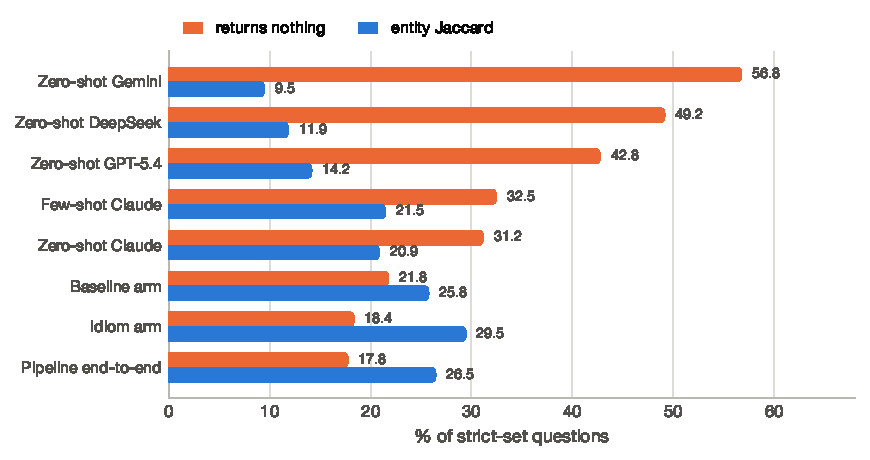
\includegraphics[width=0.8\textwidth]{figures/fig_empty_rate.pdf}
  \caption{How often each system returns nothing, against its accuracy.}
  \label{fig:empty}
  \tabnote{Every gold query on the strict set returns at least one row, so an empty result is always wrong.}
\end{figure}

\begin{figure}[H]
  \centering
  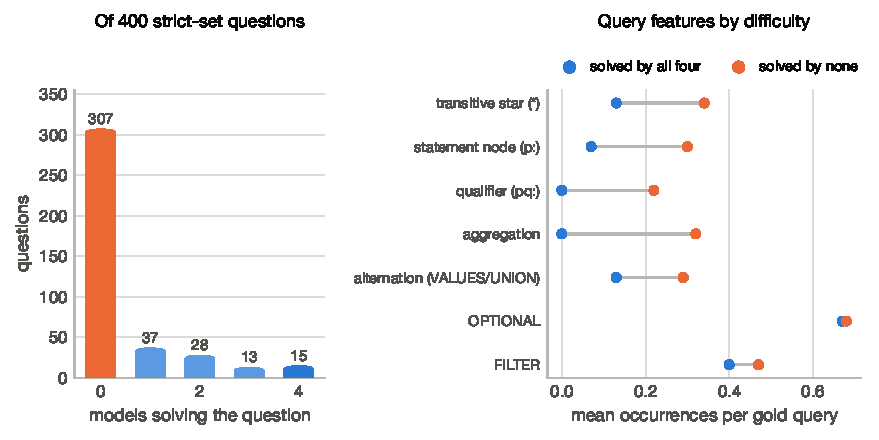
\includegraphics[width=0.8\textwidth]{figures/fig_cross_model_agreement.pdf}
  \caption{Cross-model agreement and what distinguishes the hard questions.}
  \label{fig:crossmodel}
  \tabnote{Left: how many of the four zero-shot models solve each question. Right: mean occurrences of each construct per gold query, comparing questions no model solved with those all four solved. Qualifier access and aggregation appear at exactly zero in every question all four solved.}
\end{figure}

\begin{figure}[H]
  \centering
  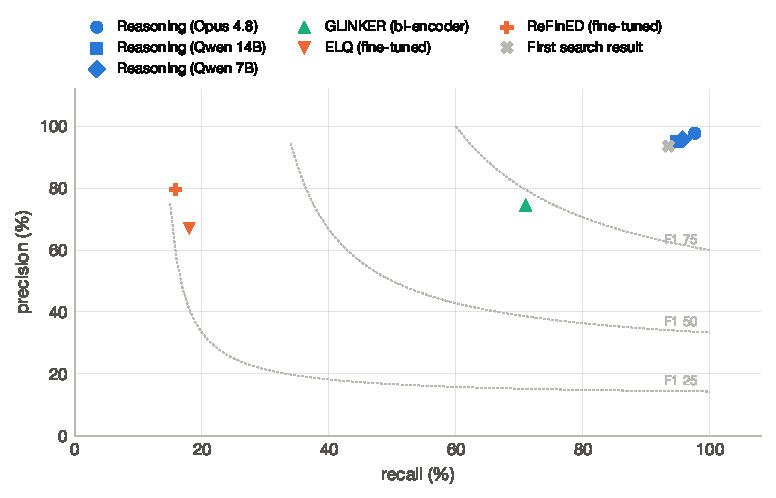
\includegraphics[width=0.8\textwidth]{figures/fig_linker_pr.pdf}
  \caption{The precision--recall signature of each linking paradigm.}
  \label{fig:linker-pr}
  \tabnote{Working split. Mention-level precision against recall for each linker.}
\end{figure}

\begin{figure}[H]
  \centering
  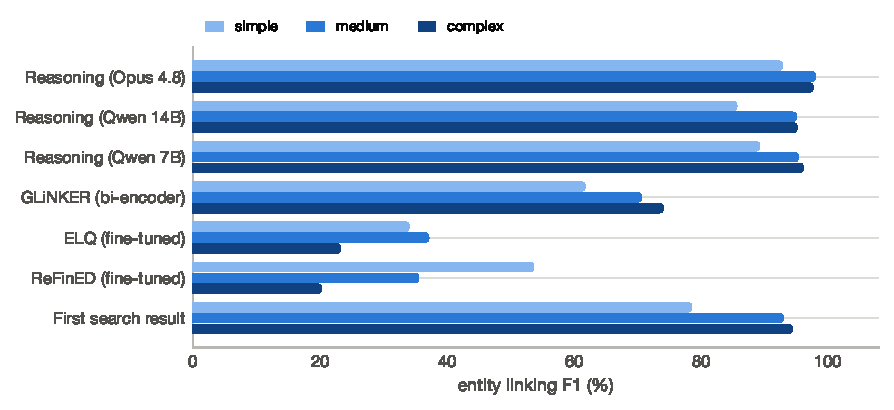
\includegraphics[width=0.8\textwidth]{figures/fig_linker_complexity.pdf}
  \caption{Linking F1 by query complexity.}
  \label{fig:linker-cx}
  \tabnote{Working split. Entity-linking F1 for simple, medium and complex queries.}
\end{figure}

\begin{figure}[H]
  \centering
  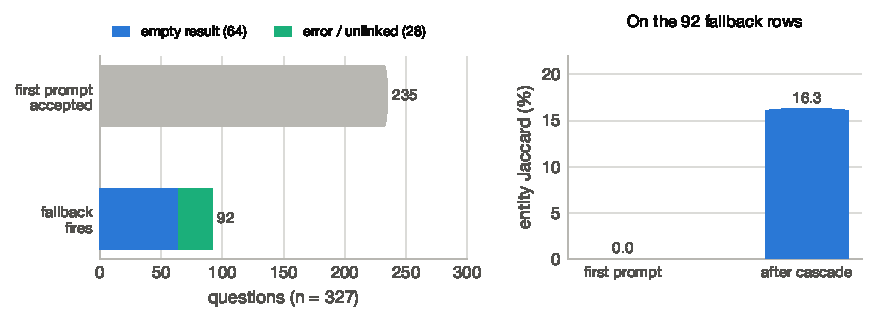
\includegraphics[width=0.8\textwidth]{figures/fig_cascade_fallback.pdf}
  \caption{Where the cascade's fallback fires, and what it recovers.}
  \label{fig:fallback}
  \tabnote{The fallback triggers on 28\,\% of questions, most often because the preferred query returned nothing. On exactly those rows the first prompt scores zero by construction.}
\end{figure}

\begin{figure}[H]
  \centering
  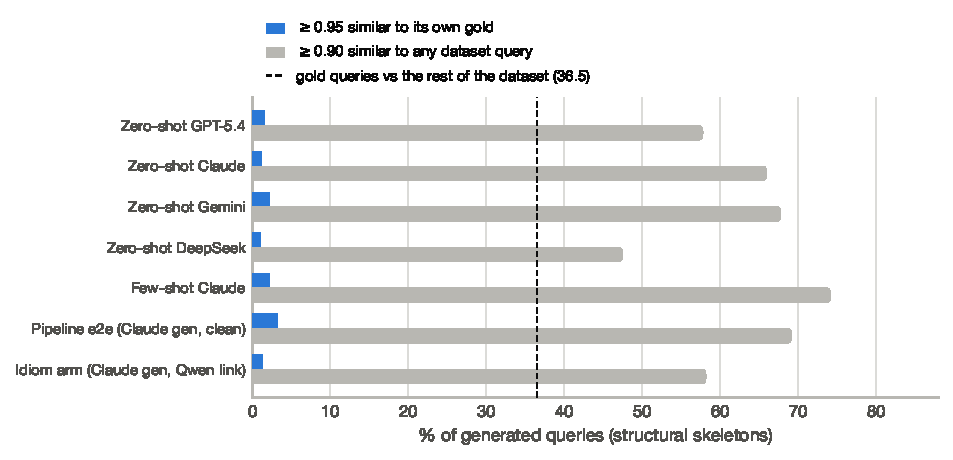
\includegraphics[width=0.8\textwidth]{figures/fig_memorisation.pdf}
  \caption{Structural similarity of generated queries to the benchmark.}
  \label{fig:memorisation}
  \tabnote{Skeletons compare query shape only.}
\end{figure}

\begin{figure}[H]
  \centering
  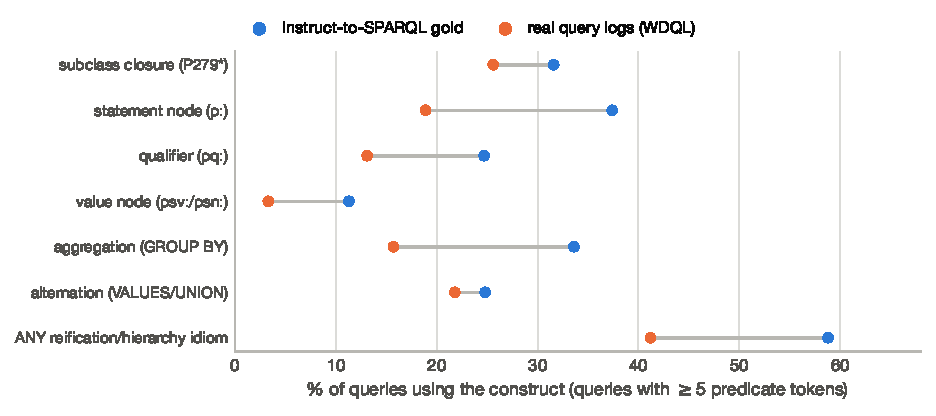
\includegraphics[width=0.8\textwidth]{figures/fig_wdql_bysize.pdf}
  \caption{Construct prevalence at matched query size.}
  \label{fig:wdql-size}
  \tabnote{Restricted to queries with at least five predicate tokens.}
\end{figure}

\begin{figure}[H]
  \centering
  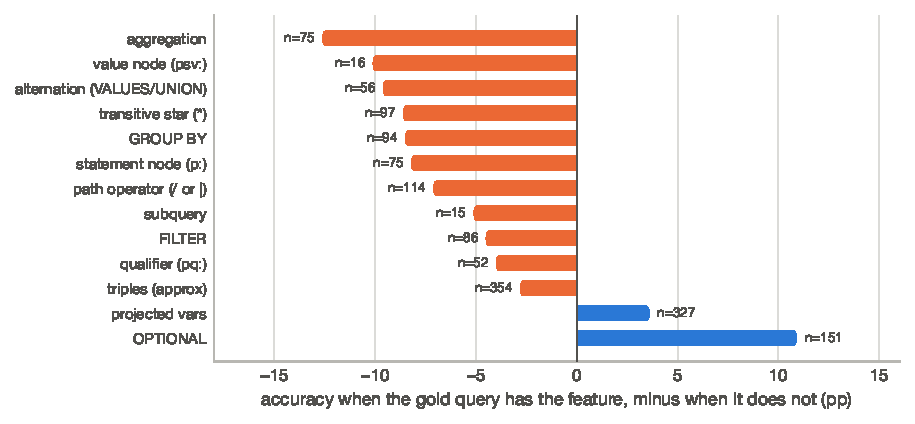
\includegraphics[width=0.8\textwidth]{figures/fig_structural_predictors.pdf}
  \caption{Gold-query features against achieved accuracy.}
  \label{fig:predictors}
  \tabnote{Group-mean differences, not predictive relationships: correlations are weak throughout ($|\rho| \leq 0.15$) and several features are rare. \textsc{optional} is the only feature associated with higher accuracy.}
\end{figure}


\ifdeclarationupfront\else
  \cleardoublepage
  \chapter*{Erklärung}
\addcontentsline{toc}{chapter}{Erklärung}

\begin{otherlanguage}{ngerman}
\noindent
Hiermit erkläre ich, dass ich die vorliegende Arbeit -- bei einer Gruppenarbeit der entsprechend gekennzeichnete Teil dieser Arbeit -- selbstständig verfasst und keine anderen als die angegebenen Quellen und Hilfsmittel benutzt wurden, und alle Stellen der Arbeit, die wortwörtlich oder sinngemäß aus anderen Quellen übernommen wurden, als solche kenntlich gemacht wurden.
Die vorliegende Arbeit hat in gleicher oder ähnlicher Form noch keiner Prüfungsbehörde vorgelegen.
Die elektronische Fassung dieser Arbeit sowie die zusätzliche elektronische Fassung in anonymisierter Form gem.\ §\,7 Abs.\,10 RPO stimmen inhaltlich überein.
\end{otherlanguage}

\vspace{2.5cm}

\noindent
Lüneburg, 15.10.2026 \hfill \makebox[6cm]{\hrulefill}\\
\phantom{Lüneburg, 15.10.2026} \hfill \makebox[6cm]{\centering Sevim Bozkurt}

\fi

\end{document}
